\documentclass{tfgitic}[2024/07/01]
% « »
% Aqui carregueu packages complementaris que necessiteu
\usepackage[utf8]{inputenc}
\usepackage{biblatex}
% \usepackage[table,xcdraw]{xcolor}
\usepackage{colortbl}
\usepackage{booktabs}
\usepackage{hhline}
\usepackage{caption}
\usepackage{bytefield}
\usepackage{tabularx}
\usepackage{xcolor}

\usepackage{makecell}
\usepackage{array}
\usepackage{graphicx}
\usepackage{multirow}
\usepackage{vcell}
\usepackage{rotating}
\usepackage{courier} % Uses Courier font for monospace


\usepackage{tikz}
\usetikzlibrary{arrows.meta, positioning, calc, decorations.markings, shapes.geometric, automata}

\usepackage{listings}
\lstdefinelanguage{JavaScript}{
  keywords={break, case, catch, const, continue, debugger, default, delete, do, else, export, finally, for, function, if, import, in, instanceof, let, new, return, super, switch, this, throw, try, typeof, var, void, while, with, yield},
  keywordstyle=\color{blue}\bfseries,
  ndkeywords={class,export,boolean,throw,implements,interface,package,private,protected,public,static,yield,await,async},
  ndkeywordstyle=\color{blue}\bfseries,
  identifierstyle=\color{black},
  sensitive=true,
  comment=[l]//,
  morecomment=[s]{/*}{*/},
  commentstyle=\color{gray}\ttfamily,
  stringstyle=\color{red}\ttfamily,
  morestring=[b]',
  morestring=[b]"
}
\lstdefinestyle{cppStyle}{
  language=C++,
  basicstyle=\scriptsize\ttfamily,     % Small font and monospaced
  numbers=left,                          % Line numbers on the left
  numberstyle=\tiny\color{gray},        % Style of line numbers
  stepnumber=1,                          % Line numbering step
  numbersep=10pt,                        % Space between numbers and code
  backgroundcolor=\color{white},        % Background color of the code
  frame=single,                          % Frame around the code
  rulecolor=\color{black},              % Frame border color
  showspaces=false,
  showstringspaces=false,
  showtabs=false,
  tabsize=4,
  captionpos=b,                         % Caption position
  breaklines=true,                      % Line breaking
  breakatwhitespace=false,
  keywordstyle=\color{blue},           % Keywords in blue
  commentstyle=\color{gray},   % Comments in gray italics
  stringstyle=\color{red},             % Strings in red
  emph={getData,setup,loop,Transport_init,Sleep_onSync,
        RoutingTable_addRoute,Sleep_setForwardNode,Sleep_init,
        scheduler_run},                         % Function names
  emphstyle=\color{purple},                    % Color for function names
}
\lstdefinestyle{jsStyle}{
    language=JavaScript,
    backgroundcolor=\color{white},   
    commentstyle=\color{gray}\itshape,   % Comments in gray italics
    keywordstyle=\color{blue},
    numberstyle=\tiny\color{gray},
    frame=single,                          % Frame around the code
    stringstyle=\color{red},             % Strings in red
    basicstyle=\ttfamily\scriptsize,
    breakatwhitespace=false,         
    breaklines=true,                 
    captionpos=b,                    
    keepspaces=true,                 
    numbers=left,                    
    numbersep=10pt,                  
    showspaces=false,                
    showstringspaces=false,
    showtabs=false,                  
    tabsize=4
}
\lstdefinestyle{bashStyle}{
  language=bash,
  backgroundcolor=\color{white},
  basicstyle=\ttfamily\footnotesize,
  keywordstyle=\color{blue},
%   commentstyle=\color{gray},
%   stringstyle=\color{red},
  showstringspaces=false,
%   columns=fullflexible,
%   keepspaces=true,
%   frame=single,
  breaklines=true,
  emph={picocom,ts,echo,cat,sudo,chmod},         % commands you want to highlight
%   emphstyle=\color{blue},
}

\renewcommand{\lstlistingname}{Codi}

\tikzstyle{startstop} = [rectangle, rounded corners, minimum width=2cm, minimum height=1cm,text centered, draw=black, fill=gray!30]
\tikzstyle{process} = [rectangle, minimum width=2, minimum height=1cm, text centered, draw=black, fill=blue!20]
\tikzstyle{decision} = [diamond, minimum width=2.5cm, minimum height=1cm, text centered, draw=black, fill=orange!30]
\tikzstyle{arrow} = [thick,->,>=stealth]

\renewcommand{\figureautorefname}{figura}
\renewcommand{\tableautorefname}{taula}
\renewcommand{\sectionautorefname}{secció}
\renewcommand{\subsectionautorefname}{apartat}
\renewcommand{\subsubsectionautorefname}{subapartat}
\renewcommand{\chapterautorefname}{capítol}
\renewcommand{\equationautorefname}{equació}


\tikzset{
  cross at end/.style={
    postaction={
      decorate,
      decoration={
        markings,
        mark=at position 1 with {
          \draw[solid, line width=0.6pt, color=black]
            (-2pt,-2pt) -- (2pt,2pt)
            (-2pt,2pt) -- (2pt,-2pt);
        }
      }
    }
  }
}

% Indica quines bd bibliografiques usarem
\addbibresource{tfe.bib}

% \title{Disseny d'un protocol LoRa amb encaminament estàtic per aplicacions de monitoratge}
\title{Disseny d'un protocol LoRa amb encaminament estàtic per aplicacions de monitoratge}
\subtitle{Aplicació en xarxes de baix consum}
% \subtitle{Adaptació per a escenaris de baix consum mitjançant sincronització temporal}

% L'autor del treball. Admet gènere (vegeu 9.2 del manual) fent \author[f]{}
\author{Pol Flotats Sabata}

% La direcció. Un treball ordinari te un o excepcionalment dos directors.
% admet gènerer i número (vegeu 9.2 del manual)
\advisor{Jordi Bonet Dalmau i Arnau Arumi Casanovas}

% Si el treball es fa sota un conveni de pràctiques (modalitat empresa)
% llavors el director (advisor) és la persona de la empresa que
% dirigeix el treball i, a més, hi ha un professor que fa de tutor (counselor).
% En aquest cas també es consigna l'empresa (company)
% \counselor admet gènere (vegeu 9.2 del manual)
%
% \counselor{}
% \company{}

% Els àmbits temàtics en que es classifica el treball. Pregunteu al
% director.
\topics{}

% Si voleu dedicatòria descomenteu
%\dedication{}

% Si voleu agraïments descomenteu
%\begin{acknowledgments}
%\end{acknowledgments}


\begin{resum}
\end{resum}

\begin{abstract}
\end{abstract}


\begin{document}
\listoffigures

% Si feu servir apèndixs, descomenteu
%\part{Memòria}

\chapter{Introducció}
\section{Objectius}
\section{Limitacions i abast del treball}
\section{Estructura de la memòria}
% primera part on es fa disseny d'un protocol genèric i NO centrat en baix consum, sinó en generalització i nodes amb taules estàtiques
% segona part on es fa un disseny centrat en baix consum i sincronització temporal

\chapter{Antecedents}
\section{Protocols de comunicació: capes i modularitat}
\label{sec:protocols}
Un protocol de comunicació defineix com dos o més dispositius d'una xarxa poden intercanviar informació. Ho fa mitjançant regles i normes que determinen la sintaxi ---format dels missatges---, la semàntica ---el seu significat---, i mecanismes de detecció i correcció d'errors.

Per tal que es pugui establir una comunicació, és necessari que els dispositius involucrats implementin el mateix protocol. Per facilitar-ho, es defineixen estàndards tècnics, publicats per organitzacions com l'\acro{iso} o l'\acro{ieee}, permetent que els fabricants puguin dissenyar dispositius compatibles. Un exemple de protocol estandaritzat és \acro{http}, amb el seu detall consultable a \cite{fielding_hypertext_2014}.

Per facilitar el disseny i implementació dels protocols, sovint es descomposen en protocols més simples. Aquests es poden agrupar en capes, on cada capa s'encarrega d'una part específica del procés de comunicació. El resultat és el que es coneix com una pila de protocols. 
En aquests dissenys, cada capa depèn de les capes inferiors per realitzar les seves funcions, i proporciona serveis a les capes superiors. El disseny i verificació de cada capa es pot fer de forma independent, i ofereixen la possibilitat d'implementar diferents protocols en cada capa, sempre que es mantingui la interfície definida entre elles.

Un dels models més coneguts és el model \acro{osi}, definit per set capes. Tot i no ser utilitzat en sistemes reals, és de gran utilitat en entorns acadèmics per comprendre la divisió per capes. Per a més informació, es pot consultar \cite{noauthor_isoiec_1994}.

En sistemes reals, el model més utilitzat és el model \acro{tcp/ip}, que estableix les bases d'Internet. Està format per quatre capes:
\begin{enumerate}
    \item \emph{Enllaç}. És la capa de més baix nivell. S'encarrega de la comunicació entre dispositius d'una mateixa xarxa ---és a dir, es poden comunicar directament---, i de la detecció i correcció d'errors produïts en la comunicació. També gestiona l'accés al medi físic per on es transmeten les dades, que sovint és compartit amb altres dispositius.
    \item \emph{Xarxa}. Gestiona la comunicació entre dispositius que es troben en xarxes diferents i, per tant, no es poden comunicar directament. Per fer-ho, s'utilitzen dispositius intermedis, coneguts com a encaminadors (\est{routers}), que determinen la ruta més eficient per fer arribar les dades al seu destí.
    \item \emph{Transport}. Defineix la connexió d'extrem a extrem entre els dispositius origen i destí i, si és necessari, que la transmissió sigui fiable. Els protocols d'aquesta capa poden oferir mecanismes com l'ordenació de missatges, l'eliminació de missatges duplicats i la gestió de congestió. Els dos protocols més coneguts d'aquesta capa són \acro{tcp}, que garanteix la transmissió fiable de dades mitjançant confirmacions i retransmissions, i \acro{udp}, que no garanteix fiabilitat, però és més eficient per aplicacions en temps real com el contingut en estríming o videjocs.
    \item \emph{Aplicació}. És la capa més alta i propera a l'usuari final. Defineix els protocols que utilitzen les aplicacions per comunicar-se a través de la xarxa, com ara \acro{http}, utilitzat per a la navegació web, o protocols de suport, com ara \acro{dns}, per a la resolució de noms de domini.
\end{enumerate}
Per a l'estàndard complet i més detall, es pot consultar \cite{braden_requirements_1989}. 

% \subsection{Referència al model TCP/IP}
\section{Tecnologia LoRa i LoRaWAN}
Els termes \emph{LoRa} i \emph{LoRaWAN} sovint es confonen i s'utilitzen ambdós termes indistintament. Mentre que el primer és una tecnologia propietària, el segon és mantingut per una associació sense ànim de lucre. En aquest apartat es presenten ambdues tecnologies, indicant-ne les seves característiques i limitacions.

\subsection{LoRa}
% // TODO: Explicar estructura missatge LoRa? Preambul?
% Mencionar mida màxima de les dades?
El nom de \emph{LoRa} prové de l'anglès \est{Long Range}. És una tecnologia de comunicació sense fils, de llarg abast, i de baix consum, fent que sigui especialment útil per a aplicacions d'Internet de les Coses (\acro{iot}). Va ser desenvolupada per \emph{Cycleo}, que va ser adquirida per \emph{Semtech} el 2012.

Utilitza freqüència sub-GHz en bandes \acro{ism} ---\emph{Industrial, Scientific and Medical}---, que són bandes de freqüència lliures de llicència. Això permet que qualsevol persona pugui utilitzar la tecnologia sense necessitat d'obtenir una llicència. Malgrat això, existeixen limitacions legals, com la potència màxima de transmissió o la quantitat de dades que es poden transmetre en un període de temps determinat. Per a més informació, es pot consultar \ref{subsec:limitacions_legals}.

Per assolir una comunicació de llarg abast, LoRa utilitza modulació de \emph{chirp spread spectrum} (\acro{css}), que permet una comunicació robusta i fiable en entorns amb interferències. Aquesta modulació es basa a codificar cada símbol com un senyal que s'escampa per tot l'ample de banda disponible, augmentant (o disminuint) de forma lineal la freqüència al llarg del temps. Gràcies al fet que la freqüència varia de forma lineal, també és resistent a l'efecte \emph{Doppler}, com s'ha estudiat a \cite{doroshkin_experimental_2019}. Una representació visual del funcionament de la modulació \acro{css} es pot veure a \cite{richard_wenner_lora_2017}.

Consta de diversos paràmetres que es poden ajustar per adaptar la comunicació a diferents necessitats:
\begin{itemize}
    \item \emph{Ample de banda}. És l'ample de banda (\acro{bw}) del canal de transmissió, sovint de \SI{125}{\kHz}, però també pot ser de \SI{250}{\kHz} o \SI{500}{\kHz}. Un ample de banda més gran permet una major velocitat de transmissió, però redueix la sensibilitat de recepció i, per tant, el rang de comunicació.
    \item \emph{Data rate}. És la velocitat de transmissió de dades (\acro{dr}), que depèn de l'ample de banda i del factor d'espargiment. Un data rate més alt permet una major velocitat de transmissió, però redueix la sensibilitat de recepció i, per tant, el rang de comunicació.
    \item \emph{Spreading Factor}. El factor d'espargiment (\acro{sf}) defineix la durada dels símbols i, per tant, la velocitat de transmissió. Es correspon amb la quantitat de bits d'informació que codifica cada símbol. Un \acro{sf} més alt permet una major sensibilitat de recepció, ja que cada símbol ocupa més temps i, per tant, és més fàcil de detectar. Això permet una comunicació a llarg abast, però redueix la velocitat de transmissió. Els valors possibles de \acro{sf} són entre 7 i 12 i, per cada increment d'1 de \acro{sf}, es redueix la velocitat de transmissió a la meitat. Una característica molt important és que els diferents \acro{sf} són ortogonals entre ells. Això implica que senyals modulats amb diferents \acro{sf} i en un mateix canal no interfereixin entre ells. 
    \item \emph{Coding Rate}. La taxa de codificació (\acro{cr}) defineix la proporció d'informació útil que es transmet en comparació amb la quantitat total de dades enviades. Els possibles valors són $\frac{4}{5}$, $\frac{4}{6}$, $\frac{4}{7}$ i $\frac{4}{8}$. Així, per un \acro{cr} de $\frac{4}{5}$, per cada quatre bits d'informació útil, se n'afegeix un de redundància.
\end{itemize}

Tots aquests paràmetres estan relacionats entre ells, i és important trobar un equilibri entre ells per aconseguir la millor comunicació possible. Per exemple, si es vol obtenir una comunicació a llarg abast, es pot augmentar el \acro{sf} i el \acro{cr}. Això reduirà la velocitat de transmissió i, per tant, augmentarà el consum energètic, ja que serà necessari estar transmetent més temps. En canvi, si es vol una comunicació ràpida, es pot reduir el \acro{sf} i augmentar el \acro{bw}, però això reduirà el rang de comunicació.

Amb una configuració adequada, es poden aconseguir comunicacions de fins a quinze quilòmetres en entorns rurals, i amb una vida útil de les bateries de diversos mesos i anys, com especifica Semtech a \cite{noauthor_lora_2024}.

Per tal que el transmissor i el receptor es puguin sincronitzar, LoRa utilitza un preàmbul de sincronització. Aquest preàmbul és un senyal de referència que permet al receptor detectar l'inici d'una transmissió i sincronitzar-se amb el transmissor. La durada del preàmbul és configurable, però sovint s'estableix de vuit símbols. Una durada major ofereix més garanties que el receptor pugui detectar la transmissió, però augmenta el temps total de transmissió i, per tant, el consum energètic.

Després de transmetre el preàmbul, es transmeten les dades del missatge. Un fet a tenir en compte és que, ja que està pensat per a ser utilitzat en dispositius de baix consum, i a la baixa velocitat de transmissió, la quantitat màxima de dades que molts transductors permeten enviar és de \SI{255}{\byte}.

Per assegurar la integritat de les dades rebudes, LoRa ofereix la possibilitat d'incloure un codi de detecció d'errors (\acro{crc}). Aquest codi es calcula a partir de les dades del missatge i s'afegeix al final del missatge. El receptor pot utilitzar aquest codi per verificar si les dades rebudes són correctes. Si el codi no coincideix amb les dades rebudes, el receptor pot descartar el missatge.


\subsection{LoRaWAN}
% // TODO: QUEDA EXPLICAR JOIN (OTAA I ABP)
Pel que fa a LoRaWAN, es tracta d'una definició de l'arquitectura d'un sistema \acro{LPWAN} (\est{Low Power Wide Area Network}), desenvolupada i mantinguda per la \href{https://lora-alliance.org}{LoRa Alliance}. Defineix el protocol de comunicació i l'arquitectura de la xarxa, així com els mecanismes de seguretat i gestió de la xarxa. 

Utilitzant l'estructura per capes vista a la \autoref{sec:protocols}, LoRaWAN opera principalment a nivell d'enllaç, malgrat que també implementa característiques d'altres capes (com ara el control de sessions). A nivell físic, utilitza la modulació LoRa.

Pel que fa a l'estructura de la xarxa, consta de 4 components principals:
\begin{itemize}
    \item \emph{Dispositius finals}. Sensors o actuadors que transmeten, a través de LoRa, missatges als \est{gateways}, conegut com a \est{uplinks}. També pot ser a l'inrevés, on els \est{gateways} transmeten missatges als dispositius finals, conegut com a \est{downlinks}.  
    \item \emph{Gateways}. Dispositius que reben els missatges dels dispositius finals i els transmeten al servidor de la xarxa. La comunicació entre els \est{gateways} i el servidor de la xarxa es realitza a través d'Internet, i no utilitza LoRa. 
    \item \emph{Servidor de la xarxa}. Dispositiu que gestiona els dispositius finals, els \est{gateways} i aplicacions de la xarxa. S'encarrega de la gestió de les comunicacions, la seguretat i la configuració dels dispositius finals. Gestionen també el xifrat punt a punt ---entre dispositius finals i servidors d'aplicació---.
    \item \emph{Servidor d'aplicació}. Processa les dades d'aplicació enviades pels dispositius finals.
\end{itemize}
Aquests dispositius es troben organitzats en una estructura d'«estrella d'estrelles», on a la part central hi trobem el servidor de la xarxa. Aquest es comunica amb múltiples \est{gateways}, i cada \est{gateway} es comunica a la vegada amb múltiples dispositius finals. 
Un fet important és que un dispositiu final no escull el \est{gateway} amb qui comunicar-se: en transmetre, tots els \est{gateways} que reben les dades ho reenvien al servidor de la xarxa. El servidor de xarxa és qui s'encarrega de detectar missatges duplicats i escollir quin és el millor \est{gateway} per transmetre un \est{downlink}. Aquesta estructura simplifica el disseny dels dispositius finals, amb el cost d'una major complexitat en el servidor de xarxa, tenint en compte que hi ha un únic servidor de xarxa per una quantitat N de dispositius finals.

Els dispositius finals poden operar en tres modes diferents, coneguts com a \emph{classes}:
\begin{itemize}
    \item \emph{Classe A}. És la classe més senzilla i de menor consum. Els dispositius finals només poden rebre missatges després d'haver realitzat una transmissió (\est{uplink}), moment en el qual obren dues finestres de recepció per rebre \est{downlinks}. Aquesta és la classe més utilitzada en aplicacions d'\acro{iot}, ja que permet un funcionament de baix consum, sent únicament necessari posar-se en mode de recepció després de fer una transmissió.
    \item \emph{Classe B}. Els dispositius finals obren finestres de recepció en moments predeterminats (coneguts com a \est{ping slots}), a més de les finestres de recepció que obren després d'un \est{uplink}. Aquest fet fa que la latència de recepció de \est{downlinks} sigui molt menor que en la classe A.
    \item \emph{Classe C}. Obren també dues finestres de recepció després d'un \est{uplink}, amb la diferència que la segona finestra es manté oberta fins la següent transmissió. Així, es pot considerar que aquests dispositius sempre estan rebent, amb l'exepció de quan transmeten. La latència de recepció de \est{downlinks} és la mínima d'entre les tres classes, però el consum energètic és màxim.
\end{itemize}

Una altra característica important de LoRaWAN és la seva capacitat d'autoajustament, conegut com a \acro{adr} (\est{Adaptative Data Rate}). Els dispositius finals poden ajustar automàticament els paràmetres de comunicació, com el \acro{sf} o la potència de transmissió, per adaptar-se a les condicions del canal de comunicació. Quan s'utilitza, el servidor de la xarxa pot indicar als dispositius finals quins paràmetres utilitzar, reduint el consum energètic i possibles interferències amb altres dispositius. Per exemple, un dispositiu molt proper a un \est{gateway} hauria d'utilitzar \acro{sf} més baixos, mentre que dispositius llunyans n'haurien d'utilitzar de més elevats.

\subsection{The Things Network}
Es tracta d'un projecte d'\acro{iot} que proporciona un servidor de xarxa públic i gratuït. El seu objectiu és crear una xarxa global de dispositius LoRaWAN, permetent la comunicació entre ells sense necessitat d'infraestructura pròpia. Els usuaris poden connectar els seus \est{gateways} a la xarxa i compartir la seva cobertura amb altres usuaris.

També ofereix la possibilitat d'afegir dispositius finals a la xarxa, i gestionar-los a través de la seva interfície web. A més, permeten la integració amb altres serveis, com ara \emph{Node-RED} o \emph{Grafana}, per visualitzar i analitzar les dades dels dispositius finals.

\subsection{Limitacions legals}
\label{subsec:limitacions_legals}
Com s'ha comentat anteriorment, LoRa utilitza bandes de freqüència lliures de llicència. Per garantir un ús adequat d'aquestes bandes, cada país estableix una sèrie de limitacions legals. Aquestes limitacions poden variar d'un país a un altre, i és important tenir-les en compte a l'hora de dissenyar un sistema de comunicació LoRa. 

Pel que fa a la Unió Europea, l'entitat responsable de la regulació de les comunicacions és l'\acro{etsi} (\est{European Telecommunications Standards Institute}). Estableix l'ús de LoRa en les freqüències entre \SI{863}{\MHz} i \SI{870}{\MHz}, amb un ample de banda màxim de \SI{250}{\kHz}.

A més, estableix un límit de potència màxima de transmissió, i un màxim d'utilització del canal. Aquestes limitacions depenen de la sub-banda utilitzada (dins el rang anteriorment mencionat), però de forma genèrica es considera una potència màxima de \SI{16}{\deci\bel\text{m}}, i una utilització màxima del canal (conegut com a \emph{duty cyle}) de l'\SI{1}{\%}. Així, per cada hora de funcionament, poden transmetre un màxim de 36 segons. Tots els detalls sobre les limitacions legals a la Unió Europea es poden consultar a \cite{etsi_etsi_nodate}.

Si s'utilitza un servidor de xarxa públic com \emph{The Things Network}, és important tenir en compte que aquest també pot aplicar limitacions addicionals. Pel que fa a \acro{ttn}, estableix una política d'ús just (\emph{fair use policy}) que limita l'ús del canal en 30 segons per dispositiu final i dia. A més, s'estableix un límit de deu \est{downlinks} per dispositiu i dia. És important tenir aquestes limitacions en compte en dissenyar un sistema; en cas d'incumpliment, el servidor de xarxa podria bloquejar l'accés del dispositiu final.

\section{Treballs relacionats}
\label{sec:treballs_relacionats}
Existeixen diversos projectes amb un objectiu similar al d'aquest treball, com ara \emph{Meshtastic} o \emph{LoRaMesher}. Tots dos projectes utilitzen LoRa per crear xarxes de comunicació entre dispositius finals, però presenten diferencies amb els objectius d'aquest treball. A més, consten també de limitacions, a les qual se'ls vol donar solució. En aquest apartat es presenten ambdós projectes, amb les seves característiques i limitacions, així com diferències vers el treball presentat. 

\subsection{Meshtastic}
Es tracta d'un projecte de codi obert que té com a objectiu crear una xarxa de comunicació descentralitzada, i pensada per a ser utilitzada en dispositius de baix consum i cost. El seu repositori es troba disponible a \href{https://github.com/meshtastic}{GitHub}.

Utilitza comunicació LoRa per a transmetre missatges entre dispositius, evitant dependre d'altres infraestructures com internet. Per tal d'aconseguir-ho, tots els dispositius actuen com a encaminadors: quan reben un missatge que no està destinat a ells, el reenvien, permetent que altres dispositius puguin repetir l'encaminament fins arribar al destí final. Una característica molt interessant d'aquest projecte és que ofereix aplicacions mòbils i web per interactuar amb els dispositius de la xarxa, permetent enviar missatges de forma molt senzilla.

L'estratègia d'encaminament que utilitza es basa en «inundació» (\est{flooding}), on cada dispositiu reenvia tots els missatges que rep, sempre que no sigui ell el destinatari, sense tenir en compte si ja els ha rebut o no. Aquest disseny tampoc considera la ubicació del destí final, fent que el missatge es transmeti per tota la xarxa. Aquests fets poden provocar un sobreús del canal, i un augment del consum energètic dels dispositius. 

Per intentar reduir aquest efecte, implementa un estil d'«inundació controlada». Quan un dispositiu rep un missatge, espera un temps proporcional a la relació senyal soroll (\acro{snr}) del missatge rebut abans de retransmetre, i cance\l.la l'enviament si un node realitza la transmissió abans. Així, un dispositiu més proper a l'origen (major \acro{snr}) esperarà més temps que un de llunyà i, per tant, el missatge el retransmetrà únicament el dispositiu llunyà. És cert que això redueix el nombre de transmissions que realitza cada dispositiu, però no evita que el missatge es retransmeti per tota la xarxa. 

Un altre inconvenient és que, a causa que els dispositius no saben quan altres dispositius realitzaran una transmissió, hagin d'estar sempre actius i en mode de recepció. Això provoca que el consum energètic dels dispositius sigui elevat (de l'ordre dels \SI{10}{\milli\watt}), fent-los poc adequats per aplicacions de monitoratge.

Durant el desenvolupament d'aquest treball, Meshtastic ha iniciat la implementació d'un protocol d'encaminament per a missatges entre dos únics dispositius. La idea d'aquest protocol és descobrir la ruta més òptima entre dos dispositius utilitzant el mecanisme d'«inundació controlada»; un cop el destí rep el missatge, respon amb un nou missatge amb la informació de la ruta, que conté tots els dispositius que han de retransmetre el missatge per arribar fins a ell. En el procés de fer arribar aquesta resposta al transmissor del missatge, tots els nodes intermedis poden generar la seva taula de rutes. En les següents transmissions, si es coneix la ruta, els missatges els reenvien únicament els nodes de la ruta. Els detalls de la implementació i funcionament d'aquest protocol es poden consultar a \cite{open_source_mesh_nodate}.

\subsection{LoRaMesher}
Es tracta d'una llibreria que implementa un protocol d'encaminament per a ser utilitzat en xarxes basades en LoRa. 

Cada dispositiu consta d'una taula d'encaminament, on es defineixen quin és el següent dispositiu a qui han d'enviar un missatge per fer-lo arribar al destí final. De forma periòdica, cada node transmet informació sobre la seva taula d'encaminament; els nodes que es troben a l'abast reben el missatge i actualitzen la seva taula d'encaminament amb la informació rebuda, no només coneixent informació sobre els seus veïns directes, sinó també sobre els veïns dels seus veïns, i així successivament. Es poden consultar els detalls d'aquesta implementació a \cite{sole_implementation_2022}.

Aquesta solució resol el problema de la «inundació controlada» presentat anteriorment, ja que únicament els nodes que es troben a la ruta reenvien el missatge. Malgrat això, presenta un dels inconvenients vists prèviament: tots els dispositius han d'estar sempre actius i en mode de recepció. Com s'ha mencionat, això provoca un consum elevat, reduint la viabilitat d'ús en aplicacions de monitoratge.

\chapter{Desenvolupament del protocol de comunicació}
En aquest capítol es presenta el disseny i implementació del protocol de comunicació. S'ha dissenyat amb l'objectiu de ser flexible, eficient, aplicable a una àmpla varietat de xarxes LoRa, i amb compatibilitat amb xarxes LoRaWAN. 

En un primer moment es fa un anàlisi de les característiques del protocol, així com la seva estructura. A continuació, es descriu l'entorn de desenvolupament i llibreries utilitzades. Seguidament, es presenta el disseny per capes del protocol, seguint l'estructura vista a la \autoref{sec:protocols}. Finalment, es mostra la implementació del protocol en un dispositiu real, i les verificacions realitzades per validar el funcionament.

No es farà especial menció a la implementació específica en codi de cada funcionalitat, si no que més bé es detallaran els criteris de disseny adoptats i les decisions preses. Es considera que, amb un disseny ben definit, la implementació del protocol és una tasca trivial. Malgrat això, es pot consultar la totalitat del codi a \url{https://github.com/pfs26/Encaminament-LoRa/tree/main/firmware}.

\section{Característiques}
El disseny del protocol està fortament influenciat pel model \acro{tcp/ip}, presentat a la \autoref{sec:protocols}. El protocol presentat es basa en una pila de protocols, on cada capa s'encarrega d'una part específica del procés de comunicació. Això permet un disseny modular, i la possibilitat de modificar les funcionalitats d'una capa sense afectar la resta.

Es basa en una xarxa de dispositius estàtics, una característica habitual en sistemes de monitoratge. Aquest fet permet prescindir de mecanismes d'encaminament dinàmic, com els presentats a la \autoref{sec:treballs_relacionats}, ja que la xarxa no canvia amb el temps, permetent simplificar el protocol. Per altra banda, això implica que la topologia de la xarxa ha de ser dissenyada abans de la seva implementació, definint les taules d'encaminament de cada dispositiu.

En utilitzar la modulació LoRa, que com s'ha dit anteriorment utilitza freqüències \acro{ism}, intenta maximitzar l'eficiència d'ús del canal. Això redueix la generació d'interferències amb altres dispositius que utilitzin el mateix canal, el nombre de retransmissions, i un menor consum energètic.

Ofereix compatibilitat amb LoRaWAN, permetent que dispositius amb connexió a \est{gateways} puguin alternar entre l'ús del protocol dissenyat o LoRaWAN. Això ofereix la possibilitat a dispositius que no tenen connexió directe a \est{gateways} de comunicar-s'hi a través de dispositius que sí que en tenen. 

Finalment, el protocol incorpora mecanismes per tal d'assegurar la correcta transmissió dels missatges a través de retransmissions automàtiques i reconeixements de missatges, semblants al protocol \acro{tcp}.

S'ha pensat per tal que totes les funcionalitats siguin configurables, permetent adaptar el protocol a les necessitats de cada aplicació. Això inclou la possibilitat d'activar o desactivar la retransmissió automàtica, així com la configuració dels paràmetres de LoRa, o intervals de temps entre retransmissions.

\section{Arquitectura del codi i comunicació entre capes}
El codi s'ha intentat organitzar de forma modular, amb la intenció de facilitar-ne la seva comprensió, manteniment, i millora, implementant cada capa del protocol com un mòdul independent. Això permet que cada capa pugui ser modificada o substituïda sense afectar la resta del protocol, facilitant la seva extensió i adaptació a diferents necessitats.

El codi es divideix en dues seccions: els fitxers de capçalera (\est{headers}) i els fitxers de codi (\est{.cpp}). Els primers contenen la definició de les funcions (consultable a la ruta \fitx{firmware/include}), mentre que els segons contenen la implementació d'aquestes funcions (\fitx{firmware/src}).

En els microcontroladors, el codi s'executa de forma cíclica, amb un bucle principal que s'executa de forma contínua. Un gran inconvenient és que no permet realitzar múltiples tasques en para\l.lel, una característica important, ja que cada capa podria haver de realitzar funcions diferents al mateix temps. Per tal d'aconseguir-ho, s'ha implementat un gestor de tasques, el qual permet executar tasques de forma periòdica, després d'un cert temps, o tan bon punt sigui possible. Malgrat no permetre l'execució para\l.lela real, aquesta solució permet simular-ho.
Amb aquesta solució, tota l'execució del protocol es realitza a través de tasques generades amb el gestor, i en el bucle principal únicament s'executa el gestor de tasques, que verifica en cada cicle l'estat de cada tasca, executant les que ho requereixen (\fitx{src/utils/scheduler.cpp}).

S'ha establert que la comunicació entre capes es realitzi a través de \est{callbacks}. Així, cada capa ofereix mètodes per permetre a una altra capa configurar una funció que s'executarà quan es produeixi un esdeveniment. Per exemple, la capa d'encaminament pot configurar una funció a la capa d'accés al medi per tal que s'executi quan es rebi un missatge. Aquesta implementació ofereix més flexibilitat, i no requereix que les capes coneguin la implementació de les altres.

Finalment, per facilitar la configuració de tot el protocol, s'ha definit un únic fitxer de configuració (\fitx{config.h}), on es poden configurar tots els paràmetres del protocol, evitant-ne la seva dispersió en diverses parts del codi.

\section{Biblioteques i entorn de desenvolupament}
Per realitzar el desenvolupament, s'han utilitzat dues llibreries externes:
\begin{itemize}
    \item \est{RadioLib}. Una llibreria que permet la comunicació sense fils a través de múltiples protocols i modulacions, incloent LoRa i LoRaWAN. Aquesta llibreria s'ha utilitzat per implementar la capa física del protocol a través de LoRa, i per comunicar-se amb \est{gateways} a través de LoRaWAN. La seva documentació es pot consultar a \cite{jan_gromes_radiolib_nodate}. 
    \item \est{TaskScheduler}. Permet la creació de tasques periòdiques, amb prioritats, o amb retard inicial, així com la seva gestió. Aquesta llibreria s'ha utilitzat per implementar el gestor de tasques, que ofereix una interfície més simple i centralitzada de la llibreria. La seva documentació es pot consultar a \cite{arkhipenko_taskscheduler_nodate}.
\end{itemize}

\section{Disseny per capes}
Com en la majoria de protocols moderns, s'ha dissenyat seguint un model per capes. L'estructura es basa en el model \acro{tcp/ip}, amb la diferència de la capa física, que el model \acro{tcp/ip} no contempla de forma explícita. 
A continuació es descriuen les diferents capes del protocol, des de la capa física fins a la capa d'aplicació, indicant-ne les funcions principals, i les decisions de disseny adoptades per optimitzar el rendiment i la simplicitat del sistema.

A la \autoref{fig:diagrama_protocols} es pot observar, de forma introductòria, com s'estructura el protocol amb les diverses capes, les quals s'explicaran amb més detall en els seus respectius apartats. 
\begin{figure}
    \centering
    \includegraphics[width=0.4\linewidth]{imatges/capesprotocol.drawio.pdf}
    \caption{Estructura per capes del protocol}
    \label{fig:diagrama_protocols}
\end{figure}

\subsection{Capa física}
La capa física és l'encarregada de transmetre la informació proporcionada per la capa superior a través del medi físic, en aquest cas, LoRa. Tot i no ser una capa que s'implementa directament en el protocol, ja que això ho realitza el transductor LoRa, s'ha considerat oportú incloure-la per una única raó: un dispositiu amb connexió amb un \est{gateway} (es considerarà «amb capacitats LoRaWAN») pot utilitzar el transductor a través de dues interfícies diferents, el protocol definit i LoRaWAN.

A causa de l'existència d'aquestes dues interfícies, és important que existeixi un mecanisme de sincronització entre les dues. En cas contrari, es podria voler realitzar una transmissió a través de LoRa quan el transductor està configurat per a LoRaWAN, o viceversa, fent que la transmissió sigui errònia.

La seva implementació és senzilla, exposant únicament dues interfícies que permeten configurar el transductor en mode LoRa o LoRaWAN, i dues més que permeten inicialitzar o deinicialitzar el transductor. La implementació es pot consultar a \fitx{lora.cpp}. 

\subsubsection{Abstracció LoRa}
Per respectar l'estructura per capes i el model de \est{callbacks} establert, s'ha dissenyat una abstracció de la llibreria RadioLib per comunicar-se entre dispositius a través de LoRa, sense utilitzar LoRaWAN.

Fent això s'obté una interfície senzilla i ben definida per a la capa superior. A més, ofereix la possibilitat de modificar el transductor utilitzat sense afectar la resta del protocol. 

La part més complexa és l'abstracció de la recepció de missatges: una recepció es pot produir en qualsevol moment, i no es pot controlar quan es realitzarà. La llibreria RadioLib ofereix la possibilitat de configurar interrupcions, fent que quan es rep un missatge es generi una interrupció en el microcontrolador. L'inconvenient de les interrupcions és que han de realitzar tasques ràpides i senzilles, per tal de no bloquejar el fil d'execució principal (si no podrien, per exemple, interrompre una transmissió en curs). La solució emprada és que la interrupció únicament guarda en un \est{flag} que s'ha produït una recepció. El fil principal, que s'executa de forma periòdica, comprova aquest \est{flag} per saber si s'ha produït una recepció i, en cas afirmatiu, l'obté i la processa. Realment, aquesta comprovació la realitza una tasca del gestor de tasques, amb una periodicitat configurable ja que, com s'ha comentat, la implementació s'ha basat en un model de tasques.

Pel que fa a les transmissions a través de LoRa, aquestes s'han hagut de dissenyar de forma bloquejant. Això implica que, quan s'utilitza la interfície de transmissió, el fil d'execució queda bloquejat fins que la transmissió s'ha completat (ja sigui correcta o incorrectament). En un primer moment es va provar de fer-ho de forma no bloquejant, fent que el transductor notifiqués quan la transmissió havia finalitzat a través d'una interrupció. A causa del fet que el transductor escollit (\acro{sx1262}) únicament permet configurar una interrupció, es va decidir que la millor solució era fer-ho de forma bloquejant, i configurar la interrupció per a la recepció de missatges, la qual no es pot controlar.

Altres mètodes que exposa la interfície permeten conèixer l'estat del canal ---si està ocupat o no---, així com establir els paràmetres de LoRa (com ara \acro{sf} o \acro{bw}) o configurar el \est{callback} de recepció. La implementació completa es pot consultar a \fitx{loraraw.cpp}.

\subsection{Accés al medi}
La funció d'aquesta capa és la gestió de l'accés al medi físic, i la comunicació entre dispositius de forma directa; és a dir, que no han d'utilitzar dispositius intermedis per comunicar-se. Un bon disseny d'aquesta capa és fonamental per garantir un ús eficient del canal, evitar interferències entre dispositius, i reduir el consum energètic. A més, és l'encarregada d'intentar garantir la integritat de les dades; és a dir, que arribin correctament al seu destí, i que les dades rebudes siguin iguals a les enviades, que no s'hagin produit errors. 

Aquesta capa es comunica amb la capa d'abstracció LoRa, rebent notificacions de recepció a través de \est{callback}, i utilitzant les seves interfícies.

\subsubsection{Estructura de les trames}
% « »
Una tasca important en qualsevol protocol és definir la forma de les dades, la «sintaxi». Així, es defineix els camps que contindrà cada missatge, i la seva longitud i posició. Per facilitat, s'ha decidit anomenar «trama» als missatges enviats per la capa d'accés al medi, sent aquest el mateix nom que s'utilitza en el model \acro{tcp/ip}.

Dos camps essencials són el \emph{receptor} i l'\emph{emissor}, que indiquen respectivament les adreces del dispositiu que rep i envia el missatge. S'ha decidit utilitzar adreces d'\SI{1}{\byte}, oferint un total de 256 adreces diferents. Malgrat això, únicament 253 són utilitzables, reservant l'adreça \fitx{0x01} per representar el \est{gateway}, la \fitx{0xFF} per un possible ús de difusió (\emph{broadcast}), i la \fitx{0x00}, per indicar l'abscència d'adreça. Aquesta quantitat de dispositius es considera suficient per a la majoria d'aplicacions de monitoratge, evitant l'ús innecessari de dades i, per tant, minimitzant el temps de transmissió i el consum energètic.

Per tal de poder identificar cada trama, s'ha inclòs un camp d'\emph{identificador} (\emph{id}), que conté un número aleatori generat per l'emissor. Aquest camp permet que el receptor pugui identificar trames duplicades i no processar-les de nou. S'ha considerat utilitzar una longitud de \SI{2}{\byte}, permetent 65536 identificadors diferents. Tot i això, s'ha reservat l'identificador \fitx{0x0000}; la utilitat d'aquest s'exposarà al \autoref{subsubsec:mac_lorawan}. En el pitjor dels casos, si 252 dispositius transmetessin a un mateix receptor, la probabilitat d'una co\l.lisió és, aproximadament, d'un 38\%. Es tracta d'un problema similar al del «problema dels aniversaris» \cite{noauthor_birthday_2025}.

Tot i semblar una probabilitat molt elevada, no es considera un fet greu: es tracta del pitjor dels casos, on 252 dispositius transmeten al mateix destí, i on el receptor recorda tots els identificadors rebuts. En aplicacions reals, la quantitat d'identificadors guardats és limitada (per exemple als últims 10), reduint la probabilitat de co\l.lisió. Si ho repetim en un cas més realista, on hi ha un receptor comú i 5 transmissors, obtenim una probabilitat de col\l.lisió del 0.015\%, i del 0.068\% si considerem 10 transmissors. Així, s'ha considerant escaient una longitud de \SI{2}{\byte}, buscant minimitzar el consum energètic i el temps de transmissió, sense afectar greument el funcionament.
% // TODO: LA FINESTRA DE RECEPCIÓ HAURIA DE GUARDAR ELS IDS JUSTOS ENTRE RETRANSMISSIONS (COSA RAPIDA A MAC)

Un altre camp important és el dels \est{flags}, que conté informació sobre el missatge. En concret, s'ha definit un camp de \SI{1}{\byte} amb els següents bits:
\begin{itemize}
    \item \emph{ACK}. Té la longitud d'un únic bit. Indica si el missatge es tracta d'un reconeixement. Si està actiu, significa que el receptor ha rebut les dades correctament, i envia aquesta informació al transmissor. En cas contrari, el missatge es considera un missatge de dades.
    \item \emph{Retry}. Té la longitud de dos bits, i indica el nombre de reintent de transmissió actual. Així, si té un valor de zero, significa que és la primera transmissió. S'ha considerat que una longitud de dos bits és suficient, permetent un màxim de quatre reintents. Es pot llegir més informació al \autoref{subsubsec:integritat}.
    \item \emph{Reservats}. Els cinc bits restants s'han reservat per a un possible ús futur. En el disseny actual no s'ha definit cap funcionalitat, però s'ha considerat oportú reservar-los per tal de poder afegir noves funcionalitats sense haver de modificar l'estructura de la trama.
\end{itemize}

També s'ha inclòs un camp de \emph{longitud}, que indica la longitud de les dades del missatge. Això permet al receptor saber quants bytes ha de llegir, i evitar llegir més bytes dels necessaris. Tenint en compte que la mida màxima d'un missatge LoRa és de \SI{255}{\byte}, podem utilitzar un únic byte per codificar la longitud.

Seguidament, es troba el camp de \emph{dades}, que conté la informació a transmetre. La seva longitud és variable, i depèn del valor del camp de longitud. A causa de la longitud màxima d'un missatge LoRa de \SI{255}{\byte}, la longitud màxima de les dades d'aquesta capa serà de \SI{248}{\byte}, sent els \SI{7}{\byte} restants per a la resta de camps. 

Per acabar, al final de la trama s'ha inclòs un camp de \acro{crc}, per intentar assegurar la integritat de les dades. S'ha optat per utilitzar un \acro{crc} de \SI{1}{\byte}, ja que la quantitat de dades que es transmeten és reduïda. De nou, saquesta decisió intenta reduir la mida del missatge final. S'ha decidit ubicar-lo al final de la trama, facilitant la tasca de càlcul i verificació: cal iterar de forma lineal la trama, sense necessitat de fer salts en memòria. A la \autoref{fig:trama_mac} es pot veure un diagrama amb l'estructura de la trama.

\begin{figure}
    \centering
    \begin{bytefield}[bitwidth=1.2em]{16}
        \bitheader{0,7,8,15} \\
        \bitbox{8}{Emissor} & \bitbox{8}{Receptor} \\
        \bitbox{16}{Identificador} \\
        \bitbox{5}{\tiny Reservats} & \bitbox{2}{\tiny Retry} & \bitbox{1}{\rotatebox{90}{\tiny ACK}} & \bitbox{8}{Longitud}\\
        \wordbox[lr]{2}{Data \tiny {(màx. \SI{248}{\byte})}} \\
        \bitbox[lrb]{8}{} & \bitbox{8}{CRC}
    \end{bytefield}
    \caption{Estructura de la trama de la capa d'accés al medi.}
    \label{fig:trama_mac}
\end{figure}
\subsubsection{Transmissió}
% « »
Quan un dispositiu vol transmetre un missatge, és primordial que no interrompi una transmissió en curs. En cas contrari, es podria produir una interferència entre ambdues transmissions, provocant que cap dels missatges arribi al seu destí. 

Per tal d'evitar co\l.lisions en l'accés al canal, es pot utilitzar una estratègia \acro{csma} (\est{Carrier Sense Multiple Access}), que consisteix a verificar si el canal està lliure abans d'iniciar una transmissió. Molts transductors LoRa incorporen la funcionalitat \acro{cad} (\est{Channel Activity Detection}), que permet detectar preàmbuls d'altres transmissions. En alguns transductors, com l'utilitzat en aquest treball, \acro{sx1262}, aquesta detecció es veu millorada, ja que també permet identificar dades del paquet LoRa, i no únicament el seu preambul, fent el procés més eficaç.

Mitjançant aquesta funcionalitat, el dispositiu comprova, a través de la interfície proporcionada per la capa d'abstracció LoRa, si hi ha una transmissió en curs. Si el canal està lliure, s'inicia la transmissió, proporcionant el missatge a la capa inferior; en cas contrari, s'aplica un mecanisme d'espera aleatori conegut com a \est{Binary Exponential Backoff} (\acro{beb}). Aquest consisteix a esperar un temps aleatori que depèn del nombre de reintents d'accés previs, multiplicant per dos el temps màxim d'espera per cada intent. Així, el rang de possibles valors ve donat per l'expressió $[0, 2^r-1]\cdot K$, on ${r}$ és el nombre de reintents realitzats, i ${K}$ una constant de temps, coneguda com a  «temps d'\est{slot}». Per exemple, si és el segon reintent d'accés al canal, i la constant és de \SI{100}{\milli\second}, el rang de temps d'espera és $[0, 2^2-1]\cdot100=[0, 300]\cdot K$ mi\l.lisegons. 

El principal avantatge d'aplicar \acro{beb} és que distribueix en el temps els reintents d'accés al canal. Això redueix la probabilitat que dos dispositius que volien accedir al canal ho reintentin en el mateix moment. Si s'utilitzés un temps d'espera constant, o que incrementés de forma lineal, es produirien co\l.lisions recurrents entre dispositius, ja que es podrien sincronitzar els temps d'accés. A més, gràcies a augmentar el possible temps d'espera exponencialment, aconseguim un mecanisme que s'adapta a l'estat del canal: en moments de molt trànsit, es distribueixen molt els temps; en canals poc ocupats, el temps d'espera és reduït.
\subsubsection{Integritat}
\label{subsubsec:integritat}
% Parlar que lora incorpora CRC. S'inclou per tal que sempre s'utilitzi CRC, fins i tot si s'utilitza lora sense CRC.
% Parlar sobre ACK
Per tal d'assegurar la correcta transmissió del missatge, s'ha implementat un mecanisme de reconeixement (\est{Acknowledgment}, \acro{ack}). Després de realitzar una transmissió, el transmissor espera rebre un missatge de reconeixement del receptor, indicant que ha rebut les dades correctament i sense errors. Si no es rep el missatge de reconeixement després d'un temps d'espera, el transmissor reintenta de nou la transmissió, incrementant el valor del camp de reintents de la trama.

El temps d'espera de recepció de l'\acro{ack} es determina a través de l'expressió $k \cdot t_{tx}$, on $t_{tx}$ és el temps de transmissió (també conegut com a \est{airtime}) del missatge, i $k$ és un factor constant major o igual a 1. Així, el temps d'espera serà, com a mínim, igual al temps de transmissió del missatge de reconeixement, per tal que el receptor el pugui enviar. Tot i això, aquest factor hauria de ser superior per considerar temps de propagació i processament. És important mencionar que el temps de transmissió es pot determinar prèviament, coneixent l'ample de banda, el factor d'espargiment i la longitud del missatge.

Una característica dels missatges de reconeixement és que l'identificador no és aleatori, sinó que és el mateix que el missatge que reconeix, l'«original». Això permet que el transmissor pugui identificar correctament l'\acro{ack}, i sapiga a quines dades fa referència. Si no fos així, el transmissor podria rebre un reconeixement d'una transmissió que havia considerat fallida, després d'haver-ne realitzat una altra; com que no sabria que fa referència a la primera, pensaria que la segona s'ha realitzat correctament. A més, el camp d'\acro{ack} dels \est{flags} està actiu, i el camp de dades no conté informació.

Pel que fa al nombre màxim de retransmissions, s'ha considerat oportú limitar-les a un màxim de tres, permetent així fins a quatre transmissions. Aquest criteri s'ha establert considerant que cada retransmissió incrementa el consum energètic, i la utilització del canal. Si després de quatre transmissions no s'ha pogut realitzar correctament la transmissió, és molt probable que les causes no siguin degudes a interferències, sinó a un error en el receptor o transmissor. En aquest cas, es considera millor cance\l.lar la transmissió i no gastar més energia.

Un altre mecanisme implementat per millorar la possibilitat d'èxit de la transmissió és l'increment automàtic de la potència de transmissió. En la primera transmissió s'utilitza la potència mínima, i per cada reintent, s'incrementa de forma lineal fins a la potència màxima. Ambdós valors de potència són configurables, permetent ajustar-se a les necessitats i regulacions locals de cada aplicació. Es va considerar també la possibilitat d'incrementar el factor d'espargiment (\acro{sf}), augmentant l'abast, seguint una estratègia similar a l'\acro{adr}. Malgrat això, no és una opció viable, ja que si el transmissor modifica aquest factor, el receptor no el podrà rebre correctament, ja que no coneix el nou factor (en LoRaWAN el \est{gateway} és capaç de rebre utilitzant múltiples \acro{sf}, fent aquesta solució factible). 

S'ha inclòs el mecanisme de detecció d'errors \acro{crc}, d'un byte de longitud. Aquest permet afegir redundància a les dades (d'\SI{1}{\byte} en aquest cas), calculat en el moment de la transmissió. Quan el receptor rep el missatge, calcula de nou el \acro{crc}, i el compara amb el rebut: si coincideixen, significa que el missatge ha arribat correctament, i s'envia el missatge de reconeixement. En cas contrari, el receptor ignora el missatge rebut, i no envia cap missatge de reconeixement. Això provoca que el transmissor reintenti la transmissió, amb el mecanisme vist anteriorment. Cal tenir en compte, però, que cap mecanisme de detecció d'errors és infalible, i pot donar falsos positius.  

Tot i que LoRa ofereix la possibilitat d'incorporar un \acro{crc}, s'ha decidit implementar un \acro{crc} propi, per tal de garantir que sempre s'utilitzi, independentment de la configuració dels transductor LoRa, millorant la integritat de les dades. 

Finalment, per evitar processar missatges duplicats, el receptor guarda en una cua els identificadors de les trames destinades a ell i que no contenen errors. Si rep un missatge amb un identificador que ja havia rebut, atura el processament de la trama, i únicament envia el missatge de reconeixement. La mida de la cua és configurable, però s'hauria de considerar el nombre màxim de reintents i el temps d'espera de recepció de reconeixement: si és massa petita, una retransmissió d'una trama ja rebuda es podria considerar un missatge nou, ja que el nombre d'altres trames vàlides rebudes entre ambdues transmissions és podria ser major a la capacitat de la cua; si és molt gran, es podrien produïr co\l.lisions d'identificadors, on dos missatges vàlids diferents tenen el mateix identificador i, com que el receptor encara recorda el primer, considera el segon com a duplicat. 
\subsubsection{Recepció}
% « »
La recepció de trames es realitza mitjançant el \est{callback} de la capa d'abstracció LoRa. En rebre una trama, es verifica el \acro{crc}; si no és correcte, s'ignora el missatge, ja que no podem assegurar que cap de les dades rebudes sigui correcta.

Seguidament es verifica si el dispositiu és el destinatari de la trama. Si no ho és, no és necessari continuar; en cas afirmatiu, es determina si la trama és de reconeixement, comprovant el bit d'\acro{ack} dels \est{flags}, i comparant l'identificador de la trama rebuda amb el de l'enviada. Si no s'havia realitzat cap transmissió prèvia, el missatge es considera un error, i s'ignora. En cas contrari, es considera que la transmissió ha estat correcta, i es notifica a la capa superior a través d'un \est{callback}. Si el missatge rebut no és un missatge de reconeixement, es guarda l'identificador a la cua de trames rebudes, i es notifica a la capa superior a través d'un \est{callback}.

S'exposa una interfície que permet a la capa superior obtenir les dades de la trama rebuda, la qual únicament s'hauria d'utilitzar després que s'hagi notificat a través de l'anterior \est{callback}. En cas contrari, les dades que s'obtinguin podrien ser incorrectes o duplicades.
\subsubsection{Cues de transmissió i recepció}
% « »
Sense la implementació d'una cua de transmissió, després d'iniciar un enviament, no seria possible realitzar-ne cap altre fins que aquest finalitzés, ja sigui per la recepció d'un \acro{ack} o per esgotament dels reintents. Això faria que la interfície de transmissió exposada a la capa superior quedés bloquejada. En conseqüència, si una capa superior volgués iniciar una nova transmissió, també hauria de quedar-se bloquejada, propagant el bloqueig cap amunt, o bé descartar l'enviament.

Per evitar-ho, s'ha implementat una cua de transmissió. Quan es vol realitzar un nou enviament, es comprova si n'hi ha una en curs: si és així, s'afegeix la trama a la cua de transmissió; en cas contrari, s'inicia directament l'enviament. Un cop finalitzada una transmissió, es comprova si hi ha més trames a la cua i, si n'hi ha, s'inicia el seu enviament.

Un aspecte important d'aquesta cua és la gestió dels reconeixements. Si un \acro{ack} es trametés a través de la cua, caldria esperar a transmetre totes les trames anteriors, fet que podria retardar excessivament el seu enviament. Això podria provocar que el transmissor considerés que la transmissió havia fallat. Per evitar-ho, els missatges de reconeixement s'envien de manera immediata, sense passar per la cua, minimitzant així el temps de resposta.

Pel que fa a la recepció, també s'ha implementat una cua. Un cop processada una trama rebuda, explicat anteriorment, aquesta es guarda a la cua i es notifica la seva arribada a la capa superior. S'hi exposen dues interfícies: una permet conèixer el nombre de trames emmagatzemades, i l'altra, obtenir les dades de la primera trama. Aquesta implementació proporciona més flexibilitat a la capa superior per gestionar els missatges rebuts, evitant el risc de sobrescriure dades rebudes prèviament.

La implementació de la cua de transmissió introdueix un problema: en notificar a la capa superior que s'ha transmès un missatge, aquesta no coneix quin missatge s'ha enviat. Per solucionar-ho, quan la capa superior inicia una transmissió, se li retorna l'identificador de la trama. Un cop s'ha enviat, el \est{callback} de fi de transmissió rep com a paràmetre l'identificador de la trama, permetent així a la capa superior saber quin missatge ha estat enviat. A més, s'afegeix un \est{callback} de transmissió errònia, que notifica a la capa superior quan no s'ha pogut realitzar una transmissió (per exemple, per esgotament de reintents), proporcionant també l'identificador de la trama.
\subsubsection{Detalls d'implementació}
La implementació d'aquesta capa s'ha realitzat mitjançant una màquina d'estats finita (\acro{fsm}). Això permet tenir un control més precís sobre l'estat de la capa, i el flux de les dades. El seu disseny, basat en les explicacions anteriors, es pot veure a la \autoref{fig:mac_fsm}.

Com la resta del protocol, s'ha implementat de forma no bloquejant ---amb l'excepció de la transmissió a través de la capa inferior, que sí que és bloquejant---, utilitzant el gestor de tasques. Aquestes s'utilitzen per programar els temps d'espera de recepció de reconeixement, i els de l'accés al canal (\acro{beb}). A més, s'han utilitzat per programar l'execució d'esdeveniments de la màquina d'estats principal. Això permet que l'execució de la \acro{fsm} no afecti altres tasques si el temps d'execució és molt llarg.

Pel que fa a la implementació de la cua, s'ha utilitzat una cua enllaçada (mitjançant una {\emph{linked list}), que permet afegir i eliminar elements de forma dinàmica, sense necessitat de conèixer prèviament la mida màxima de la cua. Aquesta implementació permet una millor gestió de la memoria, utilitzant únicament la quanitat necessària en cada moment. A més, és més eficient que una llista basada en vectors, ja que no requereix moure tots els elements quan se n'afegeix o se n'elimina un. L'única limitació és la memòria disponible del microcontrolador; de forma experimental, s'ha observat una disponibiltiat d'uns \SI{300}{\kilo\byte} en el microcontrolador ESP32-WROOM-32, que permetria emmagatzemar més de \num{3000} trames de \SI{255}{\byte} (mida màxima de la trama, comptant capçalera).

La implementació d'aquesta capa es pot trobar al fitxer \fitx{mac.cpp}, l'extensió de la capa amb funcionalitats de cua al \fitx{mac_buffer.cpp}, i la de cua enllaçada a \fitx{utils/LinkedFIFO.hpp}.
\subsubsection{LoRaWAN}
\label{subsubsec:mac_lorawan}
LoRaWAN ja defineix els mecanismes d'accés al medi i, per tant, no aplica els detalls comentats anteriorment. Malgrat això, s'ha decidit implementar una capa d'abstracció per tal de poder-la utilitzar fàcilment, i integrar-la amb l'estructura de la resta del protocol. S'ha optat per incloure-la en aquesta secció ja que implementa mecanismes d'accés al medi, i coexisteix amb la capa d'accés al medi.

S'utilitzen dispositius LoRaWAN de classe A, i la definició 1.1 del protocol LoRaWAN, la qual afegeix millores de seguretat respecte les versions \acro{1.0.x} anteriors. Es pot consultar l'especificació completa a \cite{noauthor_lorawan_2023}.

Una millora de seguretat important és que no permet la reutilització de \est{nonces}, un mecanisme que permet garantir la unicitat de les connexions a la xarxa. És a dir, evita que un tercer pugui escoltar un missatge de connexió i transmetre'l de nou, fent-se passar pel transmissor original. En les versions \acro{1.0.x} s'implementava com un valor aleatori; en la versió \acro{1.1} s'implementa com un comptador que incrementa per cada unió a la xarxa, que tant dispositiu com \est{gateway} han de recordar. Si el dispositiu utilitza un \est{nonce} ja utilitzat, el servidor de la xarxa rebutjarà la connexió. 

Aquesta millora implica la utilització de memòria no volàtil en el dispositiu, per tal de poder guardar el valor del comptador fins i tot després de reiniciar-se. Gràcies a la capa d'abstracció, la implementació d'aquest mecanisme és trivial: quan la capa superior utilitza la interfície exposada per iniciar la connexió, la capa LoRaWAN inicia la connexió, i guarda el \est{nonce} a la memòria no volàtil.

A causa de la possibilitat d'utilitzar LoRa o LoRaWAN, si després d'utilitzar LoRaWAN es canvia al mode LoRa, una següent connexió a LoRaWAN implicaria un nou procés d'inici de connexió, que pot ser lent. Per evitar-ho, després de cada transmissió es guarden els valors de sessió, que contenen comptadors d'\est{uplinks} i \est{downlinks}, i claus per encriptar els missatges, generades en unir-se a la xarxa. Els valors de sessió no s'emmagatzemen a memòria no volàtil i, per tant, després de reiniciar-se es forçarà una nova unió a la xarxa. Així, el que s'aconsegueix guardant la sessió és que els canvis entre LoRa i LoRaWAN siguin molt més ràpids, no requerint un nou procés d'unió, però sense perdre la seguretat de LoRaWAN, requerint noves unions després de reiniciar-se (com si fos un dispositiu que únicament implementa LoRaWAN).

En utilitzar dispositius de classe A, la recepció es produeix únicament després d'una transmissió. Això implica que, si una capa superior utilitza la interfície per enviar un missatge a través de LoRaWAN, aquesta també hauria de retornar les possibles dades rebudes. Aquest comportament és totalment diferent a l'establert en la resta de capes, on la capa inferior notifica a través de \est{callbacks}. Per solucionar-ho, es simula aquest comportament, i si després de realitzar una transmissió s'ha rebut un missatge, es programa una tasca ---a través del gestor de tasques--- que executarà el \est{callback} de recepció de la capa superior tan aviat com sigui possible. 

Com que LoRaWAN no utilitza el protocol d'accés al medi exposat anteriorment, l'identificador que s'assigna a les transmissions és el \fitx{0x0000}. Utilitzar sempre aquest identificador és segur, ja que com que no utilitza el protocol d'accés al medi exposat, tampoc implementa cues, i les transmissions són bloquejants, fent que no hi pugui haver dues transmissions amb el mateix identificador a la vegada. A més, cal recordar que s'havia reservat aquest identificador i, per tant, no serà mai assignat pel protocol d'accés al medi a cap trama.

Es pot consultar la implementació d'aquesta capa al fitxer \fitx{lorawan.cpp}.
\subsubsection{Situacions especials}
En aquest subapartat es descriuen diferents situacions que poden produir-se durant l'ús del protocol de transmissió, juntament amb el comportament esperat del sistema en cada cas. Conèixer aquestes situacions teòriques permet determinar si es comporta de forma adequada en situacions reals.
% \\
% \\

A la \autoref{fig:mac_tx_correcte_reintent} s'observa un exemple de transmissió correcta, amb una següent transmissió també satisfactòria després d'un reintent. Es tractaria d'una situació considerada comú, i on l'estat final dels dos dispositius és l'esperat: el dispositiu 1 realitza 2 transmissions que considera satisfactòries (ja que rep \acro{ack}), i el dispositiu 2 les ha rebut correctament.
% TX correcta + TX amb 1 reintent (no rep dades)
\begin{figure}[h]
    \centering
    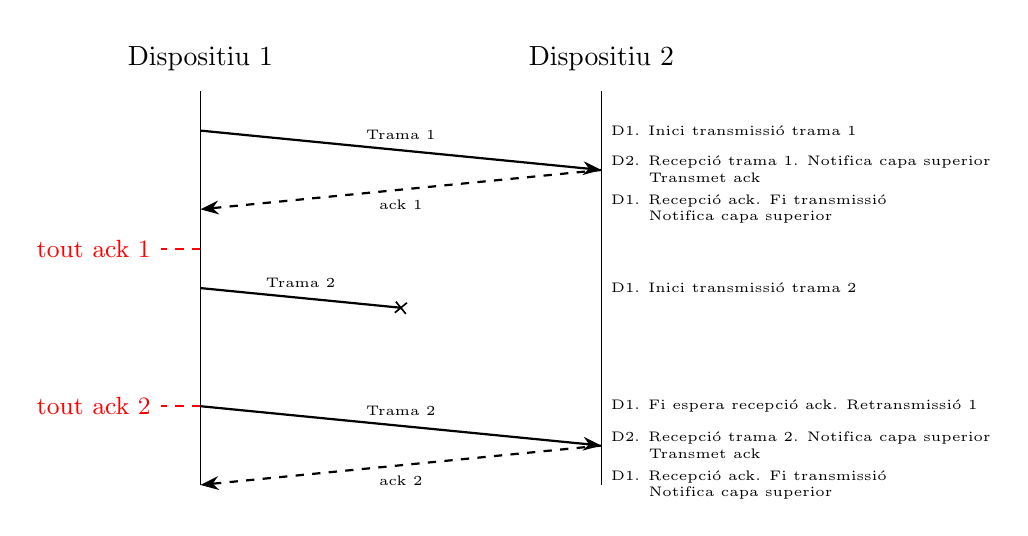
\begin{tikzpicture}[
        device/.style={draw=none, minimum width=1cm, minimum height=0.8cm},
        msg/.style={-Stealth, thick},
        ack/.style={-Stealth, thick, dashed},
        timeout/.style={red, thick, dashed},
        node distance=1cm and 3cm,
        timeline/.style={draw, dashed, white},
        fail/.style={thick, cross at end}
    ]
    
    % Devices
    \node[device] (dev1) at (0,0) {Dispositiu 1};
    \node[device, right=of dev1] (dev2) {Dispositiu 2};
    % \draw[msg] ($dev1.south$) -- ($(dev1.south)+(0,-3)$);
    \draw ($(dev1.south) + (0,0)$) -- ($(dev1.south) + (0,-5)$);
    \draw ($(dev2.south) + (0,0)$) -- ($(dev2.south) + (0,-5)$);
    
    % First message
    \draw[msg] ($(dev1.south)+(0,-0.5)$) -- ($(dev2.south)+(0,-1.0)$) node[midway, above] {\tiny{Trama 1}};
    \draw[ack] ($(dev2.south)+(0,-1.0)$) -- ($(dev1.south)+(0,-1.5)$) node[midway, below] {\tiny{\acro{ack} 1}};
    \draw[timeout] ($(dev1.south)+(0,-2)$) -- ++(-0.5,0) node[left] {\small{\acro{tout ack 1}}};
    \node[right] at ($(dev2.south)+(0,-0.5)$) {\tiny{D1. Inici transmissió trama 1}};
    \node[right] at ($(dev2.south)+(0,-0.9)$) {\tiny{D2. Recepció trama 1. Notifica capa superior}};
    \node[right] at ($(dev2.south)+(0,-1.1)$) {\tiny{\hspace{2em}Transmet \acro{ack}}};
    \node[right] at ($(dev2.south)+(0,-1.4)$) {\tiny{D1. Recepció \acro{ack}. Fi transmissió}};
    \node[right] at ($(dev2.south)+(0,-1.6)$) {\tiny{\hspace{2em}Notifica capa superior}};

    
    % Second message (fails)
    % \draw[fail] ($(dev1.south)+(0,-2.5)$) -- ($(dev2.south)+(0,-3)$) node[midway, above] {\tiny{Trama 2}};
    \draw[fail] ($(dev1.south)+(0,-2.5)$) -- ($ (dev1.south) !0.5! (dev2.south) + (0,-2.75) - (0,0) $) node[midway, above] {\tiny{Trama 2}};
    \draw[timeout] ($(dev1.south)+(0,-4)$) -- ++(-0.5,0) node[left] {\small{\acro{tout ack} 2}};
    \node[right] at ($(dev2.south)+(0,-2.5)$) {\tiny{D1. Inici transmissió trama 2}};
    
    % Retransmit message
    \draw[msg] ($(dev1.south)+(0,-4)$) -- ($(dev2.south)+(0,-4.5)$) node[midway, above] {\tiny{Trama 2}};
    \draw[ack] ($(dev2.south)+(0,-4.5)$) -- ($(dev1.south)+(0,-5)$) node[midway, below] {\tiny{\acro{ack} 2}};
    \node[right] at ($(dev2.south)+(0,-4)$) {\tiny{D1. Fi espera recepció \acro{ack}. Retransmissió 1}};
    \node[right] at ($(dev2.south)+(0,-4.4)$) {\tiny{D2. Recepció trama 2. Notifica capa superior}};
    \node[right] at ($(dev2.south)+(0,-4.6)$) {\tiny{\hspace{2em}Transmet \acro{ack}}};
    \node[right] at ($(dev2.south)+(0,-4.9)$) {\tiny{D1. Recepció \acro{ack}. Fi transmissió}};
    \node[right] at ($(dev2.south)+(0,-5.1)$) {\tiny{\hspace{2em}Notifica capa superior}};

    \end{tikzpicture}
    \caption{Transmissió correcta, i segona transmissió correcta després de reintent.}
    \label{fig:mac_tx_correcte_reintent}
\end{figure}

Una situació més excepcional és la representada a la \autoref{fig:mac_tx_considerat_fallida}, on el dispositiu 1 realitza una transmissió, sense rebre en cap retransmissió el missatge de reconeixement. Malgrat això, el dispositiu 2 sí que havia rebut la trama, generant l'\acro{ack} corresponent, el qual no arriba al dispositiu 1. S'observa com en la segona recepció de la trama, el dispositiu 2 no notifica a la capa superior, ja que ja s'havia processat prèviament. En aquesta situació, el dispositiu 1 considera que la transmissió no ha estat satisfactòria, malgrat que el dispositiu 2 sí que havia rebut la trama.

% TX incorrecte + 3 reintents - Fallada transmissió
\begin{figure}[h]
    \centering
    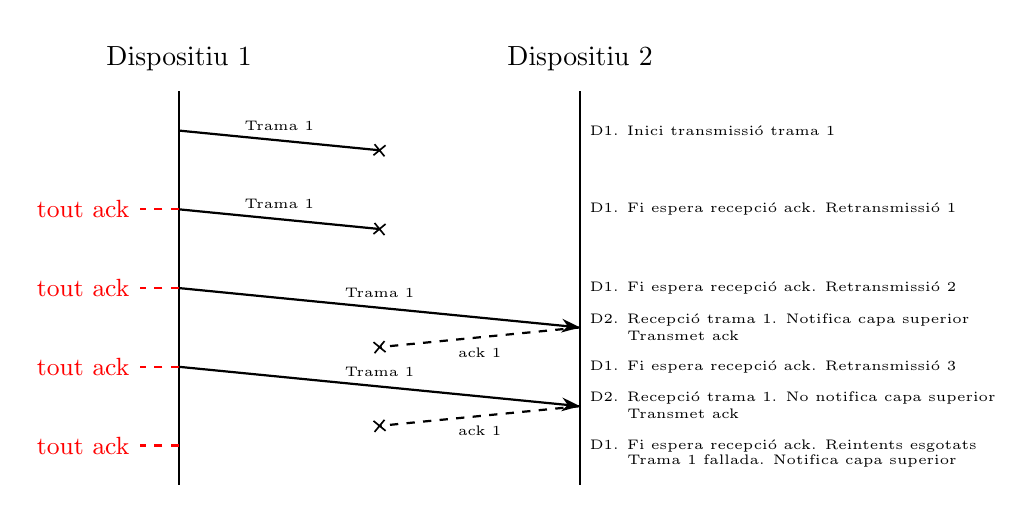
\begin{tikzpicture}[
        node distance=1cm and 3cm,
        device/.style={draw=none, minimum width=1cm, minimum height=0.8cm},
        msg/.style={-Stealth, thick},
        ack/.style={-Stealth, thick, dashed},
        timeout/.style={red, thick, dashed},
        fail/.style={thick, cross at end},
        failAck/.style={thick, cross at end, dashed},
    ]

        % Devices
        \node[device] (dev1) at (0,0) {Dispositiu 1};
        \node[device, right=of dev1] (dev2) {Dispositiu 2};
        % \draw[msg] ($dev1.south$) -- ($(dev1.south)+(0,-3)$);
        \draw ($(dev1.south) + (0,0)$) -- ($(dev1.south) + (0,-5)$);
        \draw ($(dev2.south) + (0,0)$) -- ($(dev2.south) + (0,-5)$);

        % First message
        \draw[fail] ($(dev1.south)+(0,-0.5)$) -- ($ (dev1.south) !0.5! (dev2.south) + (0,-0.75) - (0,0) $) node[midway, above] {\tiny{Trama 1}};
        \draw[timeout] ($(dev1.south)+(0,-1.5)$) -- ++(-0.5,0) node[left] {\small{\acro{tout ack}}};
        \node[right] at ($(dev2.south)+(0,-0.5)$) {\tiny{D1. Inici transmissió trama 1}};
        
        \draw[fail] ($(dev1.south)+(0,-1.5)$) -- ($ (dev1.south) !0.5! (dev2.south) + (0,-1.75) - (0,0) $) node[midway, above] {\tiny{Trama 1}};
        \draw[timeout] ($(dev1.south)+(0,-2.5)$) -- ++(-0.5,0) node[left] {\small{\acro{tout ack}}};
        \node[right] at ($(dev2.south)+(0,-1.5)$) {\tiny{D1. Fi espera recepció \acro{ack}. Retransmissió 1}};

        \draw[msg] ($(dev1.south)+(0,-2.5)$) -- ($ (dev2.south) + (0,-3) $) node[midway, above] {\tiny{Trama 1}};
        \draw[failAck] ($(dev2.south)+(0,-3)$) -- ($(dev1.south) !0.5! (dev2.south)+(0,-3.25)$) node[midway, below] {\tiny{\acro{ack} 1}};
        \draw[timeout] ($(dev1.south)+(0,-3.5)$) -- ++(-0.5,0) node[left] {\small{\acro{tout ack}}};
        \node[right] at ($(dev2.south)+(0,-2.5)$) {\tiny{D1. Fi espera recepció \acro{ack}. Retransmissió 2}};
        \node[right] at ($(dev2.south)+(0,-2.9)$) {\tiny{D2. Recepció trama 1. Notifica capa superior}};
        \node[right] at ($(dev2.south)+(0,-3.1)$) {\tiny{\hspace{2em}Transmet \acro{ack}}};

        % \node[align=left] {\tiny{This is a\\demonstration.}};

        \draw[msg] ($(dev1.south)+(0,-3.5)$) -- ($ (dev2.south) + (0,-4) $) node[midway, above] {\tiny{Trama 1}};
        \draw[failAck] ($(dev2.south)+(0,-4)$) -- ($(dev1.south) !0.5! (dev2.south)+(0,-4.25)$) node[midway, below] {\tiny{\acro{ack} 1}};
        \draw[timeout] ($(dev1.south)+(0,-4.5)$) -- ++(-0.5,0) node[left] {\small{\acro{tout ack}}};
        \node[right] at ($(dev2.south)+(0,-3.5)$) {\tiny{D1. Fi espera recepció \acro{ack}. Retransmissió 3}};
        \node[right] at ($(dev2.south)+(0,-3.9)$) {\tiny{D2. Recepció trama 1. No notifica capa superior}};
        \node[right] at ($(dev2.south)+(0,-4.1)$) {\tiny{\hspace{2em}Transmet \acro{ack}}};

        \node[right] at ($(dev2.south)+(0,-4.5)$) {\tiny{D1. Fi espera recepció \acro{ack}. Reintents esgotats}};
        \node[right] at ($(dev2.south)+(0,-4.7)$) {\tiny{\hspace{2em}Trama 1 fallada. Notifica capa superior}};

    \end{tikzpicture}
    \caption{Transmissió considerada fallida, rebuda correctament per receptor.}
    \label{fig:mac_tx_considerat_fallida}
\end{figure}

Per acabar es mostra una situació més complexa i completa, representada a la \autoref{fig:mac_tx_complet}. Es representen tres dispositius, amb la primera transmissió del dispositiu 2 completada després d'un reintent. En el procés d'espera de recepció de reconeixement, es mostra com aquest rep una trama, enviada pel dispositiu 1, i genera el corresponent \acro{ack}. Per acabar, es representa el comportament de la cua de transmissió, on el dispositiu 2 inicia una nova transmissió just després de rebre el missatge de reconeixement.

\begin{figure}[h]
    \centering
    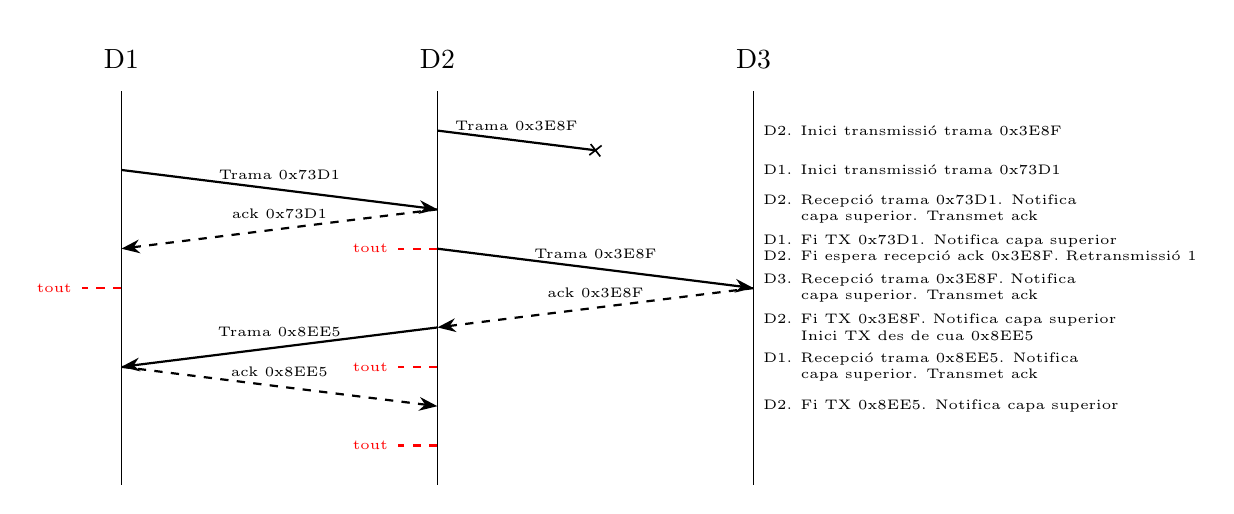
\begin{tikzpicture}[
        node distance=1cm and 3cm,
        device/.style={draw=none, minimum width=1cm, minimum height=0.8cm},
        msg/.style={-Stealth, thick},
        ack/.style={-Stealth, thick, dashed},
        timeout/.style={thick, red, dashed},
        fail/.style={thick, cross at end},
        failAck/.style={thick, cross at end, dashed},
    ]

        % Devices
        \node[device] (dev1) at (0,0) {D1};
        \node[device, right=of dev1] (dev2) {D2};
        \node[device, right=of dev2] (dev3) {D3};
        \draw ($(dev1.south) + (0,0)$) -- ($(dev1.south) + (0,-5)$);
        \draw ($(dev2.south) + (0,0)$) -- ($(dev2.south) + (0,-5)$);
        \draw ($(dev3.south) + (0,0)$) -- ($(dev3.south) + (0,-5)$);

        \draw[fail] ($(dev2.south)+(0,-0.5)$) -- ($ (dev2.south) !0.5! (dev3.south) + (0,-0.75) - (0,0) $) node[midway, above] {\tiny{Trama \fitx{0x3E8F}}};
        \draw[timeout] ($(dev2.south)+(0,-2)$) -- ++(-0.5,0) node[left] {\small{\acro{\tiny{tout}}}};
        \node[right] at ($(dev3.south)+(0,-0.5)$) {\tiny{D2. Inici transmissió trama \fitx{0x3E8F}}};

        \draw[msg] ($(dev1.south)+(0,-1)$) -- ($(dev2.south) + (0,-1.5) - (0,0) $) node[midway, above] {\tiny{Trama \fitx{0x73D1}}};
        \draw[timeout] ($(dev1.south)+(0,-2.5)$) -- ++(-0.5,0) node[left] {\small{\acro{\tiny{tout}}}};
        \node[right] at ($(dev3.south)+(0,-1)$) {\tiny{D1. Inici transmissió trama \fitx{0x73D1}}};

        \draw[ack] ($(dev2.south)+(0,-1.5)$) -- ($(dev1.south)+(0,-2)$) node[midway, above] {\tiny{\acro{ack} \fitx{0x73D1}}};
        \node[right] at ($(dev3.south)+(0,-1.4)$) {\tiny{D2. Recepció trama \fitx{0x73D1}. Notifica}};
        \node[right] at ($(dev3.south)+(0,-1.6)$) {\tiny{\hspace{2em}capa superior. Transmet \acro{ack}}};
        \node[right] at ($(dev3.south)+(0,-1.9)$) {\tiny{D1. Fi TX \fitx{0x73D1}. Notifica capa superior}};
        
        \draw[msg] ($(dev2.south)+(0,-2)$) -- ($(dev3.south) + (0,-2.5) - (0,0) $) node[midway, above] {\tiny{Trama \fitx{0x3E8F}}};
        \draw[ack] ($(dev3.south)+(0,-2.5)$) -- ($(dev2.south)+(0,-3)$) node[midway, above] {\tiny{\acro{ack} \fitx{0x3E8F}}};
        \draw[timeout] ($(dev2.south)+(0,-3.5)$) -- ++(-0.5,0) node[left] {\small{\acro{\tiny{tout}}}};
        \node[right] at ($(dev3.south)+(0,-2.1)$) {\tiny{D2. Fi espera recepció \acro{ack} \fitx{0x3E8F}. Retransmissió 1}};
        \node[right] at ($(dev3.south)+(0,-2.4)$) {\tiny{D3. Recepció trama \fitx{0x3E8F}. Notifica}};
        \node[right] at ($(dev3.south)+(0,-2.6)$) {\tiny{\hspace{2em}capa superior. Transmet \acro{ack}}};

        \draw[msg] ($(dev2.south)+(0,-3)$) -- ($(dev1.south) + (0,-3.5) - (0,0) $) node[midway, above] {\tiny{Trama \fitx{0x8EE5}}};
        \draw[ack] ($(dev1.south)+(0,-3.5)$) -- ($(dev2.south)+(0,-4)$) node[midway, above] {\tiny{\acro{ack} \fitx{0x8EE5}}};
        \draw[timeout] ($(dev2.south)+(0,-4.5)$) -- ++(-0.5,0) node[left] {\small{\acro{\tiny{tout}}}};
        \node[right] at ($(dev3.south)+(0,-2.9)$) {\tiny{D2. Fi TX \fitx{0x3E8F}. Notifica capa superior}};
        \node[right] at ($(dev3.south)+(0,-3.1)$) {\tiny{\hspace{2em}Inici TX des de cua \fitx{0x8EE5}}};
        \node[right] at ($(dev3.south)+(0,-3.4)$) {\tiny{D1. Recepció trama \fitx{0x8EE5}. Notifica}};
        \node[right] at ($(dev3.south)+(0,-3.6)$) {\tiny{\hspace{2em}capa superior. Transmet \acro{ack}}};
        \node[right] at ($(dev3.south)+(0,-4)$) {\tiny{D2. Fi TX \fitx{0x8EE5}. Notifica capa superior}};


    \end{tikzpicture}
    \caption{Transmissió considerada fallida, rebuda correctament per receptor.}
    \label{fig:mac_tx_complet}
\end{figure}
\subsubsection{Múltiples transductors}
% « »
Una situació que es podria donar és la de disposar de múltiples ràdios LoRa en un mateix dispositiu. Per exemple, podria ser útil utilitzar-ne una com a transmissora i una altra com a receptora, ambdues amb paràmetres de configuració LoRa diferents. Una altra situació d'utilitat es trobaria quan algunes transmissions s'han de realitzar amb un dispositiu més llunyà ---utilitzant un \acro{sf} més elevat---, i d'altres amb dispositius més propers, utilitzant \acro{sf} més baixos per reduir el temps de transmissió i el consum energètic.

Malgrat no ser una funcionalitat implementada, gràcies al disseny modular, afegir aquesta funcionalitat és trivial: caldria modificar la capa d'accés al medi per tal de poder seleccionar quin transductor s'ha d'utilitzar en cada moment, on cada transductor formaria part de la capa física (o de la seva abstracció).

Aquest mateix comportament es podria fins i tot obtenir amb una única ràdio, disposant de diferents perfils de configuració LoRa, i implementats com parts diferents de la capa física. A la \autoref{fig:mac_multiplesTrans} es pot observar l'estructura de capes que s'hauria d'implementar per obtenir aquesta funcionalitat.

\begin{figure}
    \centering
        \includegraphics[width=0.4\linewidth]{imatges/multiplesTXLora.drawio.pdf}
    \caption{Estructura de capes amb múltiples perfils de ràdio.}
    \label{fig:mac_multiplesTrans}
\end{figure}

% // TODO: ESTEM AQUI, QUEDA FER AIXO

\subsection{Encaminament estàtic}
La funció d'aquesta capa és la de determinar quin és el següent dispositiu a qui s'ha d'enviar un missatge perquè arribi al destí final. Tal com s'ha comentat anteriorment, s'utilitza un encaminament estàtic, de manera que les taules que defineixen les rutes s'han de configurar prèviament. Aquesta capa també és responsable de gestionar i accedir a aquestes taules quan sigui necessari.

Una altra tasca important que duu a terme és la de commutar entre l'ús del protocol definit, a través de la capa d'accés al medi, i l'ús de LoRaWAN, mitjançant la capa d'abstracció de LoRaWAN comentada anteriorment. D'aquesta manera, la capa d'encaminament es comunica amb la capa d'accés al medi, rebent notificacions de final de transmissió i de recepció de missatges a través del protocol personalitzat, i també amb la capa d'abstracció de LoRaWAN, rebent notificacions de recepció de missatges a través de LoRaWAN.

\subsubsection{Estructura dels paquets}
És necessari que aquesta capa pugui saber quin és el destí final del missatge, per tal de determinar quin és el següent dispositiu a qui s'ha d'enviar. Per tant, ha de contenir un camp amb l'adreça del dispositiu de \emph{destí}. També s'inclou l'adreça del dispositiu \emph{emissor}, permetent saber d'on s'ha originat el missatge. Ambdós camps tenen la mateixa longitud que els de la capa d'accés al medi, és a dir, \SI{1}{\byte}, la qual cosa permet reutilitzar les mateixes adreces en les dues capes i simplifica la implementació.

Per tal d'evitar transmissions infinites ---per exemple, si una ruta resulta en un bucle--- s'afegeix un camp de \acro{ttl} (\est{Time To Live}), que indica el nombre màxim de salts que pot fer un missatge abans de ser descartat. Per exemple, si l'emissor genera un missatge amb un \acro{ttl} d'1, aquest només podrà ser transmès al següent dispositiu de la ruta. El camp \acro{ttl} ocupa \SI{1}{\byte}, permetent un màxim de 255 salts. Tenint en compte que la xarxa està limitada a un màxim de 253 dispositius, aquesta longitud és suficient, ja que no haurien d'existir rutes de longitud superior al màxim de dispositius.

Per acabar, s'ha inclòs un camp de \emph{longitud}, que indica la longitud de les dades del missatge. Com en el protocol d'accés al medi, permet saber quants bytes s'han de llegir per obtenir les dades. Es reserva també un byte, ja que la longitud màxima de les dades del protocol d'accés al medi és de \SI{248}{\byte}. Així, les \emph{dades} podran tenir una longitud màxima de \SI{244}{\byte}, sent els \SI{4}{\byte} restants per a la resta de camps.

Seguint el model \acro{tcp/ip}, el missatges d'aquesta capa s'anomenen \emph{paquets}. La seva estructura, amb els camps prèviament esmentats, es pot observar a la \autoref{fig:paquet_encaminament}.

\begin{figure}
    \centering
    \begin{bytefield}[bitwidth=1.2em]{16}
        \bitheader{0,7,8,15} \\
        \bitbox{8}{Origen} & \bitbox{8}{Destí} \\
        \bitbox{8}{TTL} & \bitbox{8}{Longitud} \\
        \wordbox{3}{Data \tiny {(màx. \SI{244}{\byte})}}
    \end{bytefield}
    \caption{Estructura del paquet de la capa d'encaminament estàtic.}
    \label{fig:paquet_encaminament}
\end{figure}
\subsubsection{Gestió de la taula d'encaminament}
% comentar que implementa interfície per afegir/eliminar taules, per si mai es defineix un mecanisme d'encaminament dinàmic
La taula d'encaminament és l'encarregada de definir quin és el següent dispositiu al qual s'ha d'enviar un paquet per tal que arribi al seu destí final. Per simplicitat, s'ha optat per permetre una única ruta per a cada dispositiu, establint així una relació un a un entre cada adreça de destí i el següent salt. Això limita la mida màxima de la taula d'encaminament a 254 entrades (253 dispositius i un \est{gateway}). A la \autoref{tab:taula_encaminament} es mostra un exemple de taula d'encaminament, on es pot veure que el dispositiu té comunicació directa amb els dispositius \fitx{0x4E} i \fitx{0xA1}, i si es vol enviar un paquet al \est{gateway}, aquest s'ha de fer arribar a través de \fitx{0x4E}.

\begin{table}
    \centering
    \begin{tabular}{p{3cm}<{\centering}p{3cm}<{\centering}}
        \toprule
        \textbf{Destí} & \textbf{Següent salt} \\
        \midrule
        \fitx{0x01} & \fitx{0x4E} \\
        \fitx{0x4E} & \fitx{0x4E} \\
        \fitx{0x12} & \fitx{0xA1} \\
        \fitx{0xA1} & \fitx{0xA1} \\
        \bottomrule    
    \end{tabular}
    \caption{Exemple taula d'encaminament.}
    \label{tab:taula_encaminament}
\end{table}

\begin{figure}
    \centering
    \begin{bytefield}[bitwidth=0.5em]{32}
        \bitheader{0,7,15,23,31,39} \\
        \bitbox{8}{\fitx{0x01}} & \bitbox{8}{\fitx{0x4E}} & \bitbox{8}{\fitx{0x4E}} & 
        \bitbox{8}{\fitx{0x4E}} & \bitbox{8}{\fitx{0x12}} & \bitbox{8}{\dots} 
    \end{bytefield}
    \caption{Representació emmagatzematge de la taula d'encaminament.}
    \label{fig:emmgatzematge_taula_encaminament}
\end{figure}

Una propietat important de la taula d'encaminament és que aquesta ha de ser persistent. Això vol dir que si el dispositiu es reinicia, aquest ha de poder recuperar la taula d'encaminament anteriorment configurada. En cas contrari, com que no es genera de forma dinàmica, aquesta capa quedaria inoperativa. Per evitar-ho, s'utilitza de nou la memòria no volàtil \acro{NVS}. La mida màxima de la taula serà de \SI{508}{\byte} (254 entrades, 2 adreces d'\SI{1}{\byte} per entrada), fet que no és problema en el dispositiu utilitzat (ESP32).

Per evitar fer lectures a la memòria \acro{nvs} per a cada consulta de ruta, es carrega tota la taula a la memòria volàtil en inicialitzar la capa, fent que les lectures siguin molt més ràpides. El format d'emmagatzematge consisteix en una seqüència de bytes, on cada parell representa una entrada: el primer byte indica l'adreça de destí i el segon, el següent salt. Aquest format facilita el bolcat de la taula entre memòria volàtil i no volàtil, ja que no cal fer cap conversió. A la \autoref{fig:emmgatzematge_taula_encaminament} es pot observar com s'emmagatzemaria part de la taula d'encaminament representada anteriorment. 

S'han implementat interfícies per afegir, eliminar i actualitzar entrades de la taula d'encaminament. Tot i que no són estrictament necessàries per al protocol d'encaminament estàtic, poden resultar útils si en el futur es vol implementar un encaminament dinàmic. En aquest cas, després de fer una modificació de la taula de rutes, s'actualitza la taula a la memòria \acro{nvs}, per tal de garantir la seva persistència.

La implementació s'ha fet en un mòdul independent, consultable al fitxer \fitx{routing_table.cpp}, permetent que sigui reutilitzable en altres possibles protocols d'encaminament.
\subsubsection{Transmissió}
\label{subsubsec:routing_tx}
Quan es vol realitzar una transmissió d'un paquet a un destí final, es realitza una consulta a la taula d'encaminament per determinar quin és el següent salt:
\begin{itemize}
    \item Si el següent salt és el \est{gateway}, representat amb l'adreça \fitx{0x01}, es realitza la transmissió del paquet a través de la capa d'abstracció de LoRaWAN.
    \item Si el següent salt és un altre dispositiu, es realitza la transmissió a través de la capa d'accés al medi.
\end{itemize}

Pel que fa al valor de \acro{ttl}, s'assigna el valor configurat per defecte (definit en temps de compilació), que depèn de la mida de la xarxa i de cada situació, però que cal recordar que està limitat a 255.

És important recordar que la capa d'accés al medi implementa una cua de transmissió, i que notifica a la capa d'encaminament quan la transmissió ha acabat. Per aquest motiu, la capa d'encaminament ofereix també la possibilitat de notificar a la capa superior de la finalització d'una transmissió, proporcionant de nou l'identificador. Aquestes notificacions (generades a través de \est{callback}) únicament es generaran per transmissions originades per la capa superior. És a dir, si la capa d'encaminament inicia una transmissió (per exemple, per encaminar un paquet rebut a través de la capa d'accés al medi), no es notificarà a la capa superior, ja que aquesta transmissió no s'hi ha originat. Aquest filtrat es pot realitzar guardant l'identificador de les trames transmeses (obtingut a través de la capa d'accés al medi) en una cua únicament si s'originen per la capa superior.

A més, cal també tenir en compte que la capa d'accés al medi implementa notificacions per transmissions fallides. De nou, aquesta notificació únicament es propagarà a la capa superior si el paquet s'hi havia originat, i no és una transmissió fallida d'un paquet encaminat. 

És també important recordar que les transmissions mitjançant LoRaWAN són bloquejants. Així, l'estat de la transmissió es coneix en el mateix moment en que s'inicia la transmissió a través de la capa d'abstracció. Per mantenir la coherència amb la resta de capes, s'implementen notificacions de transmissió simulades, programant les notificacions de transmissió correcta i fallida a través del gestor de tasques.
\subsubsection{Recepció}
\label{subsubsec:routing_rx}
% « »
Quan la capa d'accés al medi notifica a la capa d'encaminament la recepció d'un paquet, mitjançant el \est{callback} corresponent, aquesta rep el paquet i verifica quin és el seu destí final. Si n'és el destí final, es notifica a la capa superior perquè el processi i es dona per finalitzat el procés. En canvi, si el paquet no és per a ell, es consulta la taula d'encaminament per determinar quin és el següent salt.

Si no existeix cap entrada a la taula per a l'adreça de destí del paquet rebut, aquest es descarta. Encara que podria semblar lògic generar un missatge de «no-reconeixement» per informar l'emissor, s'ha decidit no implementar aquest mecanisme. Fer-ho implicaria assignar tasques a la capa d'encaminament, que van més enllà de determinar la ruta del paquet. A més, aquest tipus de notificació incrementaria el nombre de transmissions, fet no desitjat en un protocol de baix consum. Tampoc hauria de ser necessari si la configuració de les taules d'encaminament s'ha realitzat correctament, ja que les rutes no canvien dinàmicament.

Si el valor del \acro{ttl} del paquet rebut és 1 (i el paquet no és per ell, verificat prèviament), es descarta el paquet, ja que no pot fer més salts. En cas contrari, es decrementa el valor del \acro{ttl} i es transmet el paquet al següent salt a través de la capa d'accés al medi o de LoRaWAN, segons correspongui.

Gràcies a la capa d'abstracció de LoRaWAN, que implementa la recepció de paquets a través de notificacions per \est{callback}, no hi ha diferència entre la recepció d'un paquet a través de LoRaWAN o a través del protocol personalitzat. En ambdós casos, la capa d'encaminament rep el paquet i realitza les mateixes operacions, explicades anteriorment.

Com s'ha comentat anteriorment, la finalització de la transmissió d'aquest paquet encaminat no es notificarà a la capa superior, ja que no s'hi ha originat.
\subsubsection{Detalls d'implementació}
La implementació d'aquesta capa no s'ha basat en una màquina d'estats perquè no és necessari mantenir cap estat entre transmissions ni recepcions. En aquest cas, el comportament de la capa d'encaminament és totalment síncron, permetent basar la implementació com una seqüència de mètodes i condicions. Basar la implementació en una \acro{fsm} requeriria un disseny més complex, sense aportar cap avantatge. 
 
A la \autoref{fig:routing_flux_tx} i a la \autoref{fig:routing_flux_rx} es mostren dos diagrames de flux, representant la transmissió i recepció de paquets respectivament. Ambdós diagrames es basen en el disseny exposat en els subapartats anteriors. A la \autoref{fig:routing_flux_txdone} es mostra el diagrama de flux de la transmissió completada, on es pot observar la notificació a la capa superior si aquesta s'hi havia originat. 

De nou, es vol destacar la diferència per evitar notificar a la capa superior d'una transmissió d'un paquet encaminat ---no generat localment---. En la transmissió d'un paquet (\autoref{fig:routing_flux_tx}), es guarda l'identificador generat per la capa d'accés al medi; en el cas d'un encaminament, no.

La implementació d'aquesta capa es troba disponible al fitxer \fitx{routing.cpp}.

\begin{figure}
    \centering
        \includegraphics[width=0.9\linewidth]{imatges/Routing_FluxTX.drawio.pdf}
    \caption{Diagrama de flux de transmissió.}
    \label{fig:routing_flux_tx}
\end{figure}

\begin{figure}
    \centering
        \includegraphics[width=0.9\linewidth]{imatges/Routing_FluxRX.drawio.pdf}
    \caption{Diagrama de flux de recepció.}
    \label{fig:routing_flux_rx}
\end{figure}

\begin{figure}
    \centering
        \includegraphics[width=0.35\linewidth]{imatges/Routing_FluxOnTX.drawio.pdf}
    \caption{Diagrama de flux de transmissió completada.}
    \label{fig:routing_flux_txdone}
\end{figure}

\subsubsection{Exemples de comunicació}
En aquest subapartat es presenten dos exemples de comunicació de la capa d'encaminament, on es representen els mecanismes prèviament explicats. Com en el cas de la capa d'accés al medi, saber quin ha de ser el comportament teòric a través de representacions gràfiques ajuda a entendre millor el funcionament, i a detectar possibles errors en la implementació. 

En ambdós exemples es representen tres dispositius, on el tercer té capacitats LoRaWAN i comunicació amb un \est{gateway}. Per simplicitat, no es representen els missatges de reconeixement, ni els reintents de transmissió, ja que aquests són responsabilitat de la capa d'accés al medi, com s'ha vist en els seus diagrames. Tampoc s'han representat els retards de transmissió dels paquets, considerant-los un aspecte del comportament del canal i, per tant, de la capa d'accés al medi. Per distingir una transmissió a través de la capa d'accés al medi i una a través de LoRaWAN, s'ha utilitzat una línia contínua per a la primera i una línia discontínua per a la segona.

Les taules d'encaminament de cada dispositiu i exemple es representen a la \autoref{tab:routing_taula_enc_exemples}.

\begin{table}[h!]
    \centering
    \begin{tabular}{c c}
        \begin{tabular}{r|ccccc}
            \multicolumn{6}{c}{\small Exemple 1} \\
            \hline
            \multicolumn{1}{c|}{\vcell{}} & \vcell{\textbf{0x01}} & \vcell{\textbf{0x02}} & \vcell{\textbf{0x03}} & \vcell{\textbf{0x04}} & \vcell{\textbf{0x05}} \\[-\rowheight]
            \multicolumn{1}{c|}{\printcellmiddle} & \printcellbottom & \printcellbottom & \printcellbottom & \printcellbottom & \printcellbottom \\ 
            \hline
            \textbf{0x01} & - & 0x04 & 0x04 & 0x04 & - \\
            \textbf{0x02} & 0x03 & - & 0x03 & 0x03 & 0x03 \\
            \textbf{0x03} & 0x04 & 0x02 & - & 0x04 & - \\
            \textbf{0x04} & 0x01 & 0x03 & 0x03 & - & -
        \end{tabular}
        &
        \begin{tabular}{r|cccc}
            \multicolumn{5}{c}{\small Exemple 2} \\
            \hline
            \multicolumn{1}{c|}{\vcell{}} & \vcell{\textbf{0x01}} & \vcell{\textbf{0x02}} & \vcell{\textbf{0x03}} & \vcell{\textbf{0x04}} \\
            [-\rowheight]
            \multicolumn{1}{c|}{\printcellmiddle} & \printcellbottom & \printcellbottom & \printcellbottom & \printcellbottom  \\ 
            \hline
            \textbf{0x01} & -    & 0x03 & 0x03 & 0x04 \\
            \textbf{0x02} & 0x03 & -    & 0x03 & 0x03 \\
            \textbf{0x03} & 0x01 & 0x02 & -    & 0x01 \\
            \textbf{0x04} & 0x01 & 0x01 & 0x01 & -
        \end{tabular}
    \end{tabular}
    \caption{Matrius d'encaminament d'exemple. La ce\l.la $(x, y)$ indica el dispositiu que $y$ ha d'utilitzar per enviar un paquet a $x$.}
    \label{tab:routing_taula_enc_exemples}
\end{table}


A la \autoref{fig:routing_encaminament_basic_gateway} es mostra un exemple bàsic. Primerament el dispositiu \fitx{0x02} vol enviar un paquet al \fitx{0x04}: obté la ruta per aquest, transmetent-ho a \fitx{0x03}. Aquest rep el paquet, verifica el \acro{ttl}, i obté la següent ruta, que és \fitx{0x04}, el qual rep el paquet, comprova que és el destí final, i ho notifica a la capa superior. 

Un segon exemple de transmissió es realitza quan \fitx{0x02} vol enviar un paquet al \est{gateway}. El dispositiu 2 consulta la taula d'encaminament i veu que el següent salt és el dispositiu 3. Aquest rep el paquet i consulta la seva taula, veient que el següent salt és el \est{gateway}. En rebre el paquet a través de LoRaWAN, realitza la transmissió dels paquets en les finestres de recepció que el dispositiu \fitx{0x04} obre, en tractar-se d'un dispositiu de classe A. Es realitza l'encaminament d'aquest nou paquet, amb el mateix mecanisme que anteriorment.

Per acabar, es representa també com un paquet amb fi de temps de vida (\acro{ttl}) és descartat, de la mateixa manera que un paquet que no pot ser encaminat, ja que no existeix cap entrada a la taula d'encaminament del dispositiu. 

\begin{figure}[h]
    \centering
    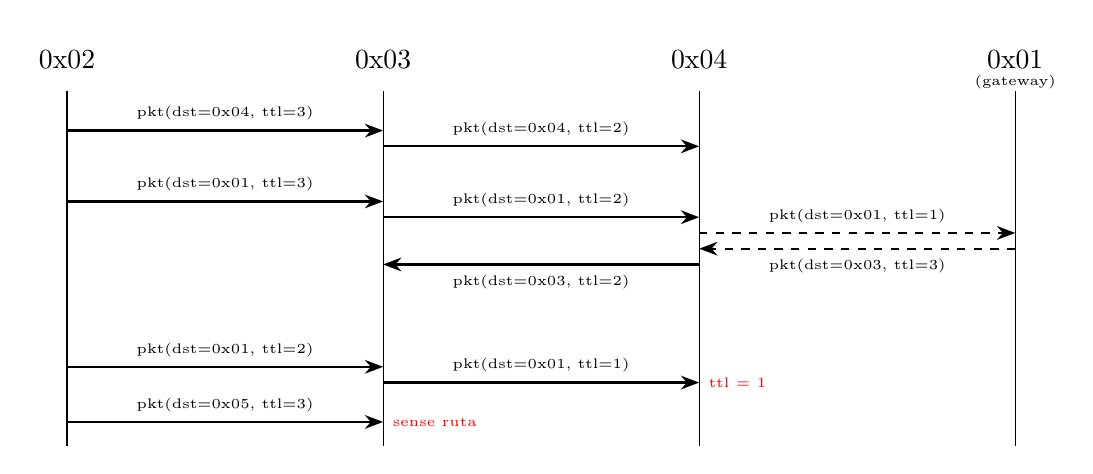
\begin{tikzpicture}[
        device/.style={draw=none, minimum width=1cm, minimum height=0.8cm},
        msg/.style={-Stealth, thick},
        wan/.style={-Stealth, thick, dashed},
        timeout/.style={red, thick, dashed},
        node distance=1cm and 3cm,
        timeline/.style={draw, dashed, white},
        fail/.style={thick, cross at end}
    ]
    
    % Devices
    \node[device] (dev1) at (0,0) {\fitx{0x02}};
    \node[device, right=of dev1] (dev2) {\fitx{0x03}};
    \node[device, right=of dev2] (dev3) {\fitx{0x04}};
    \node[device, right=of dev3] (gw) {\fitx{0x01}};

    \node[above] at ($(gw.south)+(0,-0.1)$) {\tiny(\est{gateway})};

    \draw ($(dev1.south) + (0,0)$) -- ($(dev1.south) + (0,-4.5)$);
    \draw ($(dev2.south) + (0,0)$) -- ($(dev2.south) + (0,-4.5)$);
    \draw ($(dev3.south) + (0,0)$) -- ($(dev3.south) + (0,-4.5)$);
    \draw ($(gw.south) + (0,0)$) -- ($(gw.south) + (0,-4.5)$);

    
    \draw[msg] ($(dev1.south)+(0,-0.5)$) -- ($(dev2.south)+(0,-0.5)$) node[midway, above] {\tiny{pkt(dst=\fitx{0x04}, ttl=3)}};
    \draw[msg] ($(dev2.south)+(0,-0.7)$) -- ($(dev3.south)+(0,-0.7)$) node[midway, above] {\tiny{pkt(dst=\fitx{0x04}, ttl=2)}};

    \draw[msg] ($(dev1.south)+(0,-1.4)$) -- ($(dev2.south)+(0,-1.4)$) node[midway, above] {\tiny{pkt(dst=\fitx{0x01}, ttl=3)}};
    \draw[msg] ($(dev2.south)+(0,-1.6)$) -- ($(dev3.south)+(0,-1.6)$) node[midway, above] {\tiny{pkt(dst=\fitx{0x01}, ttl=2)}};
    \draw[wan] ($(dev3.south)+(0,-1.8)$) -- ($(gw.south)+(0,-1.8)$) node[midway, above] {\tiny{pkt(dst=\fitx{0x01}, ttl=1)}};
    \draw[wan] ($(gw.south)+(0,-2)$) -- ($(dev3.south)+(0,-2)$) node[midway, below] {\tiny{pkt(dst=\fitx{0x03}, ttl=3)}};
    \draw[msg] ($(dev3.south)+(0,-2.2)$) -- ($(dev2.south)+(0,-2.2)$) node[midway, below] {\tiny{pkt(dst=\fitx{0x03}, ttl=2)}};

    \draw[msg] ($(dev1.south)+(0,-3.5)$) -- ($(dev2.south)+(0,-3.5)$) node[midway, above] {\tiny{pkt(dst=\fitx{0x01}, ttl=2)}};
    \draw[msg] ($(dev2.south)+(0,-3.7)$) -- ($(dev3.south)+(0,-3.7)$) node[midway, above] {\tiny{pkt(dst=\fitx{0x01}, ttl=1)}};
    
    \draw[red] ($(dev3.south)+(0,-3.7)$) node[right] {\tiny{\acro{ttl = 1}}};

    \draw[msg] ($(dev1.south)+(0,-4.2)$) -- ($(dev2.south)+(0,-4.2)$) node[midway, above] {\tiny{pkt(dst=\fitx{0x05}, ttl=3)}};

    \draw[red] ($(dev2.south)+(0,-4.2)$) node[right] {\tiny{\acro{sense ruta}}};

    % \node[right] at ($(dev2.south)+(0,-1.6)$) {\tiny{\hspace{2em}Notifica capa superior}};

    
    \end{tikzpicture}
    \caption{Exemple encaminament bàsic amb \est{gateway} LoRaWAN.}
    \label{fig:routing_encaminament_basic_gateway}
\end{figure}

Una altra situació més complexa es pot produir quan la xarxa es troba separada en dues xarxes, amb un \est{gateway} LoRaWAN al mig. En aquest cas, el comportament és similar a l'observat anteriorment, on el \est{gateway} fa les transmissions dels paquets únicament després de rebre'n un altre, ja que es tracten de dispositius de classe A. Així, si un dispositiu vol enviar un paquet a un dispositiu de la xarxa contrària, la correcta transmissió d'aquest paquet dependrà de la transmissió d'un altre paquet originat a la xarxa contraria, per tal que pugui obrir la finestra de recepció necessària.

A més, es requereix també un servidor d'aplicació, encarregat de processar els paquets que el \est{gateway} rep, i generar els \est{downlinks} corresponents. Malgrat aquests requisits, aquest exemple permet i\l.lustrar les capacitats d'encaminament de la capa, que no tenen perquè estar limitades a una única xarxa. El seu diagrama es pot trobar representat a la \autoref{fig:routing_encaminament_complex_gateway}.

\begin{figure}[h]
    \centering
    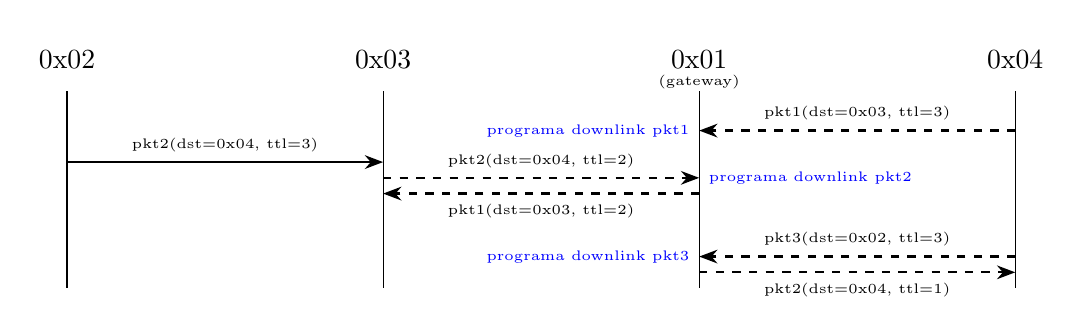
\begin{tikzpicture}[
        device/.style={draw=none, minimum width=1cm, minimum height=0.8cm},
        msg/.style={-Stealth, thick},
        wan/.style={-Stealth, thick, dashed},
        timeout/.style={red, thick, dashed},
        node distance=1cm and 3cm,
        timeline/.style={draw, dashed, white},
        fail/.style={thick, cross at end}
    ]
    
    % Devices
    \node[device] (dev1) at (0,0) {\fitx{0x02}};
    \node[device, right=of dev1] (dev2) {\fitx{0x03}};
    \node[device, right=of dev2] (gw) {\fitx{0x01}};
    \node[device, right=of gw] (dev3) {\fitx{0x04}};

    \node[above] at ($(gw.south)+(0,-0.1)$) {\tiny(\est{gateway})};

    \draw ($(dev1.south) + (0,0)$) -- ($(dev1.south) + (0,-2.5)$);
    \draw ($(dev2.south) + (0,0)$) -- ($(dev2.south) + (0,-2.5)$);
    \draw ($(gw.south) + (0,0)$) -- ($(gw.south) + (0,-2.5)$);
    \draw ($(dev3.south) + (0,0)$) -- ($(dev3.south) + (0,-2.5)$);


    \draw[wan] ($(dev3.south)+(0,-0.5)$) -- ($(gw.south)+(0,-0.5)$) node[midway, above] {\tiny{pkt1(dst=\fitx{0x03}, ttl=3)}};
    \draw[blue] ($(gw.south)+(0,-0.5)$) node[left] {\tiny{\acro{programa downlink pkt1}}};
    
    \draw[msg] ($(dev1.south)+(0,-0.9)$) -- ($(dev2.south)+(0,-0.9)$) node[midway, above] {\tiny{pkt2(dst=\fitx{0x04}, ttl=3)}};
    \draw[wan] ($(dev2.south)+(0,-1.1)$) -- ($(gw.south)+(0,-1.1)$) node[midway, above] {\tiny{pkt2(dst=\fitx{0x04}, ttl=2)}};
    \draw[blue] ($(gw.south)+(0,-1.1)$) node[right] {\tiny{\acro{programa downlink pkt2}}};
    \draw[wan] ($(gw.south)+(0,-1.3)$) -- ($(dev2.south)+(0,-1.3)$) node[midway, below] {\tiny{pkt1(dst=\fitx{0x03}, ttl=2)}};

    \draw[wan] ($(dev3.south)+(0,-2.1)$) -- ($(gw.south)+(0,-2.1)$) node[midway, above] {\tiny{pkt3(dst=\fitx{0x02}, ttl=3)}};
    \draw[blue] ($(gw.south)+(0,-2.1)$) node[left] {\tiny{\acro{programa downlink pkt3}}};
    \draw[wan] ($(gw.south)+(0,-2.3)$) -- ($(dev3.south)+(0,-2.3)$) node[midway, below] {\tiny{pkt2(dst=\fitx{0x04}, ttl=1)}};
    \end{tikzpicture}
    \caption{Exemple encaminament entre xarxes separades per \est{gateway} LoRaWAN.}
    \label{fig:routing_encaminament_complex_gateway}
\end{figure}



\subsection{Capa de transport}
La funció d'aquesta capa és la de gestionar la transmissió de missatges entre el dispositiu transmissor, l'origen, i el receptor final, el destí. A més, també ofereix la possibilitat d'implementar un mecanisme de fiabilitat, intentant garantir que el missatge arribi correctament al destí final, i que no es rebin missatges duplicats. 

Cal diferenciar aquest mecanisme de fiabilitat del que ofereix la capa d'accés al medi, que únicament intenta garantir que el missatge arribi correctament al següent salt. Després de realitzar els intents màxims de retransmissió, el missatge es descarta si no s'ha pogut transmetre. La capa de transport, en canvi, incorpora mecanismes de fiabilitat amb una visió global, indiferentment dels mètodes que apliquen les capes inferiors.

La gestió de la recepció de missatges duplicats és també una qüestió important en xarxes encaminades. La transmissió d'un missatge es podria realitzar a través de diferents rutes, arribant al destí final per múltiples camins. És essencial poder identificar cada missatge i descartar els duplicats, assegurant així una comunicació coherent. 

A més, s'encarrega també de gestionar els missatges de les diferents aplicacions que poden existir a la capa d'aplicació, redirigint cada missatge a la seva aplicació corresponent.


\subsubsection{Estructura dels segments}
Seguint l'estructura del model \acro{tcp/ip}, els missatges d'aquesta capa s'anomenen \emph{segments}, permetent diferenciar-los dels paquets de la capa d'encaminament, o de les trames de la capa d'accés al medi. 

Per tal de poder identificar cada missatge, i evitar duplicitats, s'inclou un \emph{identificador} de missatge. S'ha dissenyat d'una longitud de \SI{2}{\byte}, permetent així un màxim de \num{65535} missatges diferents. La distinció entre aquest identificador i el de la capa d'accés al medi és que aquest és global, mantenint-se des de l'emissor fins al receptor final. En canvi, l'identificador de la capa d'accés al medi és local, i es reinicia cada vegada que es realitza una nova transmissió. Així, la probabilitat de co\l.lisió d'identificadors és menor que en la capa d'accés al medi, ja que la quantitat d'identificadors generats és menor. Malgrat això, s'ha optat per mantenir la mateixa longitud d'identificador, reduïnt la probabilitat de co\l.isió d'identifiadors en aquesta capa, incrementant així la fiabilitat d'extrem a extrem. 

El mecanisme de fiabilitat és semblant a l'implementat a la capa d'accés al medi, on el receptor reconeix la recepció del missatge a través d'un missatge de reconeixement. Així, és necessari disposar d'un camp d'\acro{ack}. Per oferir la possibilitat d'utilitzar o no aquest mecanisme, s'ha inclòs un camp que indica la so\l.licitud del reconeixement. Ambdós camps d'han implementat com un únic bit, inclosos dins un camp de \est{flags}. Així, el camp de \est{flags} ocupa \SI{1}{\byte}, utilitzant un bit pel camp \emph{ACKRequest}, i un per \emph{ACKResponse}.

Per gestionar el redireccionament de segments cap a l'aplicació corresponent de la capa superior s'ha inclòs un camp per identificar l'aplicació, conegut com a \emph{port} en el model \acro{tcp/ip}. Per tal d'aprofitar l'espai disponible del segment, s'han utilitzat els sis bits restants del camp de \est{flags}, permetent un màxim de 64 aplicacions diferents. 

Per acabar, inclou els camps de \emph{longitud} i de \emph{dades}. Tenint en compte que un paquet pot tenir una longitud màxima de dades de \SI{244}{\byte}, i que el segment formarà part d'aquestes dades, la longitud màxima del segment serà de \SI{240}{\byte}. Així, el camp de dades, té una longitud màxima de \SI{240}{\byte}, sent els \SI{4}{\byte} restants per a la resta de camps. La longitud del camp de \emph{longitud} és d'\SI{1}{\byte}, suficient per a representar aquesta longitud màxima.

A la \autoref{fig:segment_transport} es pot observar l'estructura del segment de la capa de transport, amb els camps comentats anteriorment.

\begin{figure}
    \centering
    \begin{bytefield}[bitwidth=1.2em]{16}
        \bitheader{0,7,8,15} \\
        \bitbox{16}{Identificador} \\
    \bitbox{6}{Port} & \bitbox{1}{\tiny \rotatebox{90}{ACK}\rotatebox{90}{Req}} & \bitbox{1}{\tiny \rotatebox{90}{ACK}\rotatebox{90}{Resp}} & \bitbox{8}{Longitud} \\
    \wordbox{3}{Data \tiny {(màx. \SI{240}{\byte})}}
    \end{bytefield}
    \caption{Estructura del segment de la capa de transport.}
    \label{fig:segment_transport}
\end{figure}
\subsubsection{Transmissió}
Com en la capa d'encaminament, la transmissió en la capa de transport és simple: utilitza la interfície exposada per la capa d'encaminament. En finalitzar la transmissió, la capa d'encaminament notificarà a través d'un \est{callback} aquesta finalització. Com en la capa d'accés al medi, el mètode de generació de l'identificador és aleatori.

La complexitat recau en la gestió de la fiabilitat. La transmissió d'un segment es pot realitzar de forma no fiable o fiable. En el primer cas, el dispositiu no espera cap reconeixement, i únicament utilitza la interfície de la capa d'encaminament per realitzar la transmissió, despreocupant-se del resultat. En el segon cas, el dispositiu espera rebre un segment de reconeixement, transmès pel receptor final. En cas de no rebre'l en un temps determinat, es retransmet de nou el segment. 

A causa de la cua de transmissió a la capa d'accés al medi, l'inici del temps d'espera de recepció del reconeixement no es pot iniciar després d'utilitzar la interfície de la capa inferior, ja que la transmissió no té per què produir-se immediatament. Així, només es pot iniciar el temporitzador quan la capa inferior notifica la transmissió del segment, a través del \est{callback} corresponent.

Per permetre aquest comportament, es guarda informació addicional d'una transmissió, en una estructura de metadades:
\begin{itemize}
    \item \emph{PDU}. Conté el \emph{Protocol Data Unit}, és a dir, el segment complet, incloent les dades i capçaleres.
    \item \emph{ID}. L'identificador assignat per la capa d'accés al medi, amb el qual es podrà identificar la transmissió en els esdeveniments de fi de transmissió o de transmissió errònia.
    \item \emph{RX}. L'adreça del receptor del segment.
    \item \emph{isSent}. Un booleà per indicar si el segment ja s'ha enviat o no. S'actualitza quan es rep la notificació de fi de transmissió.
    \item \emph{ackTimeout}. Indica l'instant de temps en mi\l.lisegons en què finalitza l'espera de reconeixement. 
    \item \emph{Reintents}. Indica el nombre de reintents de transmissió que s'han realitzat per un segment.
    \item \emph{Tasca}. Tasca del gestor de tasques que s'encarrega de gestionar el temporitzador d'espera del reconeixement. Permet cance\l.lar la tasca si es rep el reconeixement.
\end{itemize}

Així, quan finalitza la transmissió d'un segment fiable, es determina en quin instant finalitza el temps d'espera de recepció de l'\acro{ack}, i es guarda a les metadades. A més, es crea una tasca que generarà l'esdeveniment de fi d'espera d'\acro{ack} quan es compleixi el temps d'espera, la qual també es guarda a les metadades, permetent cance\l.lar-la si es produeix el reconeixement. Més informació sobre la fiabilitat es pot trobar al \autoref{subsubsec:transport_fiabilitat}.

Les metadades es guarden tant per a transmissions fiables com no fiables. Malgrat no ser necessari determinar el temps d'espera d'un reconeixement en un segment no fiable, guardar les metadades és útil per poder notificar a la capa superior.

Les notificacions implementades en aquesta capa són similars a les de la capa d'encaminament: fi de transmissió i error de transmissió.
\begin{itemize}
    \item En segments fiables, la notificació de fi de transmissió es genera quan s'ha rebut el reconeixement per part del receptor. En cas contrari, si no es rep el reconeixement i s'esgoten els intents de transmissió, es genera una notificació d'error de transmissió.
    \item En segments no fiables, la notificació de fi de transmissió es genera quan la capa d'accés al medi ha pogut lliurar el segment al següent salt. Aquesta notificació no garanteix la recepció del segment per part del receptor final, i únicament indica que s'ha pogut transmetre. D'altra banda, si la capa d'accés al medi notifica que no s'ha pogut transmetre, es genera un notificació d'error de transmissió, indicant que el segment no s'ha pogut transmetre ni al següent salt.
\end{itemize}
Aplicar notificacions en un segment no fiable pot semblar contradictori, però pot ser útil per a les aplicacions que volen saber si el segment, com a mínim, s'ha pogut transmetre des del dispositiu. Utilitzant LoRa, les transmissions poder ser lentes, i aquest tipus de notificacions poden oferir una alternativa més llegura.
\subsubsection{Recepció}
Es produeix una recepció d'un segment quan la capa inferior, la d'encaminament, ho notifica a través del \est{callback} configurat. Quan es rep un segment, es verifica el camp \emph{ACKRequest} dels \est{flags}. En cas que el segment rebut so\l.liciti un reconeixement, es genera un segment amb el camp \emph{ACKResponse} actiu, i es transmet cap al transmissor de l'anterior segment, utilitzant el mecanisme exposat en el subapartat anterior.

Seguidament es verifica si el segment s'havia rebut anteriorment, consultant el camp d'identificador del segment rebut amb els identificadors dels últims segments rebuts. Aquest disseny és similar a l'utilitzat a la capa d'accés al medi, on es guarden les últimes trames rebudes. De nou, la mida d'aquesta cua és configurable, però s'ha de tenir en compte que si és massa petita, es poden produir falsos positius, i si és massa gran, hi podrien haver co\l.lisions d'identificadors de segments diferents.

Si ja s'havia rebut anteriorment l'identificador, ja que existeix a la cua de segments rebuts, s'atura el processament del segment, i es descarta. En cas contrari, es guarda l'identificador a la cua, i es notifica a la capa superior de la recepció d'un nou segment.
\subsubsection{Gestió de múltiples aplicacions}
% hi poden haver múltiples capes superiors (aplicacions)
% A quina cal enviar les notificacions?
Una característica d'aquesta capa és que pot disposar de múltiples capes superiors, o aplicacions. Això permet que cada aplicació pugui gestionar els seus propis missatges, els quals poden tenir estructures diferents, sense interferir entre elles. 

Per a implementar aquest comportament, és necessari que la capa de transport conegui les interfícies a través de les quals notificar la recepció o transmissió d'un missatge per a cada aplicació. Per fer-ho, es dissenya una taula de ports, on cada port s'associa a les funcions de notificació específiques per a cada aplicació. Aquesta taula permet utilitzar múltiples \emph{callbacks} per gestionar la recepció i la fi de transmissió de segments, amb un \emph{callback} dedicat a cada aplicació. A la \autoref{tab:taula_ports} es pot observar un exemple de taula de ports, on es pot veure com tres aplicacions diferents poden gestionar la recepció i transmissió de segments a través de les seves propies interfícies.

\begin{table}
    \begin{tabular}{cccc}
        \toprule
        \textbf{Port} & \textbf{Transmissió} & \textbf{Error transmissió} & \textbf{Recepció} \\
        \midrule
        \fitx{00} & \fitx{TxDone1()} & \fitx{TxErr1()} & \fitx{Rx1()} \\
        \fitx{17} & \fitx{TxDone2()} & \fitx{TxErr2()} & \fitx{Rx2()} \\
        \fitx{63} & \fitx{TxDoneN()} & \fitx{TxErrN()} & \fitx{RxN()} \\
        \bottomrule
    \end{tabular}
    \centering
    \caption{Exemple de taula de ports.}
    \label{tab:taula_ports}
\end{table}

Així, quan es rep un segment amb el port 17, la capa de transport utilitzarà la interfície \fitx{Rx2} per notificar la recepció del segment únicament a l'aplicació interessada.

La taula de ports pot tenir fins a un màxima de 64 entrades, una per cada possible port. Per cada un d'aquests, es pot assignar únicament una interfície de notificació, garantint així que una única aplicació sigui notificada. En cas que no s'hagi assignat cap interfície a un port, la capa de transport no podrà notificar-ho, fent que l'esdeveniment es perdi.

Un altre problema de disposar de múltiples capes superiors és que cada aplicació pot intentar inicialitzar la capa de transport. Per evitar-ho, és important que la capa de transport guardi l'estat d'inicialització i, en cas que es vulgui inicialitzar de nou, simplement ho «simuli», sense realitzar cap acció addicional. Aquest mateix mecanisme cal aplicar-lo també a la deinicialització: en cas que una aplicació intenti deinicialitzar la capa de transport, cal verificar que no hi ha cap altra aplicació que la utilitzi, i en cas que sí, no realitzar cap acció addicional. Així, es garanteix que la capa de transport es pot inicialitzar i deinicialitzar múltiples vegades, sense interferir amb les aplicacions que la utilitzin.
\subsubsection{Fiabilitat}
\label{subsubsec:transport_fiabilitat}
% « »
Com s'ha comentat anteriorment, la implementació de la fiabilitat es basa en un mecanisme de reconeixement, similar al de la capa d'accés al medi.
Quan s'ha realitzat la transmissió d'un segment fiable, s'inicia un temporitzador a través del gestor de tasques, que genera un esdeveniment quan finalitza el temps d'espera d'\acro{ack}. Quan es produeix aquest esdeveniment, s'obtenen les metadades de la transmissió, i es reintenta la transmissió de nou, repetint el procediment.

És important destacar que, si no es pot realitzar la transmissió del segment (per exemple, perquè la capa d'accés al medi no pot transmetre), s'aplicarà el mateix mecanisme. En aquest cas, la capa inferior ho notifica a través del \est{callback} de transmissió errònia, en lloc del de fi de transmissió.

Per tal de poder identificar quin segment un missatge de reconeixement ---aquell que té el camp \emph{ackResponse} actiu--- reconeix, s'estableix que l'identificador d'aquests segments sigui el mateix que el del segment original, el que reconeixen. Així, en rebre un recnoeixement, la capa de transport pot consultar la llista de metadades, que conté l'identificador del segment original, i així poder identificar el segment i aturar el temporitzador d'espera d'\acro{ack}.

El temps d'espera de recepció del reconeixement no és fix, sinó que depèn del nombre de retransmissions que s'han realitzat anteriorment, seguint una funció exponencial. Gràcies a això, el temps d'espera s'incrementa com més reintents s'han realitzat, ajustant-se a les condicions de la xarxa.
Aquest temps ve determinat per l'expressió $k\cdot 2^r$, on \emph{k} és un valor constant i configurable, i \emph{r} el nombre de reintents realitzats. El valor de \emph{k} cal configurar-lo adequadament per evitar generar \est{timeouts} prematurs, i per evitar un excés de temps d'espera:
\begin{itemize}
    \item Hauria de verificar $k\ge (2n-1)\cdot t_{tx}$, on \emph{n} és el nombre de dispositius en la ruta més llarga de la xarxa, sense incloure el dispositiu emissor. És així ja que cada node ha de realitzar una transmissió al següent salt del segment (d'aquí el factor \emph{n}), i també haurà de fer-ho pel missatge de reconeixement del receptor final (d'aquí el factor \emph{2}). A més, cal recordar que l'inici del temps d'espera s'inicia després de transmetre el segment al següent salt, d'aquí el terme \emph{-1}.
    \item Hauria de considerar el temps d'una transmissió a través de LoRaWAN. Si la transmissió d'un segment té com a destí el \est{gateway}, el dispositiu amb capacitats LoRaWAN haurà, abans de generar el segment de reconeixement, transmetre les dades a través de LoRaWAN. Aquest temps depèn de la configuració del canal i de l'\acro{adr}, fent que sigui difícil d'establir ja que no es coneix prèviament. De forma experimental, s'ha observat com pot introduir un retard de múltiples segons, sent adequat deixar un marge de mínim 5 segons. 
\end{itemize}
Aquest criteri estableix el temps mínim d'espera, considerant que per a cada dispositiu de la ruta es requereix únicament una transmissió, i que el retard de processametn és nul. Si s'estableix un temps mínim d'espera menor a aquest, és segur que es produiran \est{timeouts} prematurs.

Establir un límit superior pel temps d'espera no és trivial. Caldria tenir en compte el nombre de retransmissions màximes de la capa d'accés al medi, i la congestió de la xarxa, que pot introduir retards a causa del \acro{beb} aplicat. 
\subsubsection{Detalls d'implementació}
La implementació de la cua dels últims identificadors de segments rebuts s'ha realitzat a través d'una cua circular, de mida màxima configurable. Gràcies a l'ús d'aquesta, la capa de transport únicament s'encarrega d'afegir nous elements, i la cua circular elimina de forma automàtica els més antics. La seva implementació es pot consultar a \fitx{utils/RingBuffer.cpp}.

Apareix una qüestió important en els missatges de reconeixement quan el destí és el \est{gateway}. Com s'ha mencionat anteriorment, aquests s'encarreguen de retransmetre els missatges rebuts al servidor de xarxa LoRaWAN, i no tenen capacitat de generar missatges. Així, hauria de ser un servidor d'aplicació qui processés el missatge rebut i, llavors, programés l'enviament d'un \est{downlink} amb el segment de reconeixement a través del \est{gateway}.
Malgrat semblar una solució vàlida, cal recordar que s'utilitzen dispositius de classe A, els quals només poden rebre missatges després de realitzar una transmissió. Així, l'enviament del missatge de reconeixement no es realitzaria fins que el dispositiu transmetés un nou missatge, un \est{uplink}. Aquest comportament afegeix molta latència, i faria dependre el missatge de reconeixement de la transmissió d'un nou missatge.

La solució que s'ha implementat és considerar el dispositiu amb capacitats LoRaWAN ---es pot comunicar amb el \est{gateway}--- com una «extensió» del \est{gateway}. Així, quan aquest fa un encaminament a través de LoRaWAN, la capa d'encaminament genera també l'esdeveniment de recepció de nou segment, permetent a la capa de transport processar el segment prèviament rebut, i generar el missatge de reconeixement en cas de ser necessari.

Aquesta solució no és la més elegant, i implica que un dispositiu que no és el destí final processi el segment rebut. No obstant això, si es veu el dispositiu amb capacitats LoRaWAN com un dispositiu diferent a la resta, considerant-lo, com s'ha dit anteriorment, com una «extensió» del \est{gateway}, la solució és vàlida per evitar que la correcta transmissió d'un segment depengui de la transmissió d'un de diferent. Gràcies a la llibreria de RadioLib, que ja incorpora mecanismes de fiabilitat a través de LoRaWAN ---també mitjançant reconeixements---, no és necessari implementar-ho manualment.

\subsubsection{Exemples de comunicació}
En aquest subapartat es presenta un exemple de comunicació, representant les característiques d'aquesta capa. Per simplicitat, es dona per suposat que les taules d'encaminament es troben ben definides i, com en els exemples d'encaminament, no es representen els temps de propagació ni de transmissió, així com els missatges de reconeixement de la capa d'accés al medi. A més, tampoc s'inclouen els identificadors dels ports de cada segment, ja que no són rellevants per a les situacions exposades, i únicament s'utilitzen en les notificacions a la capa superior.

A la \autoref{fig:transport_exemple_1} es representa el diagrama de l'exemple. El dispositiu \fitx{0x02} inicia una transmissió fiable cap al dispositiu \fitx{0x03}; aquest no rep el reconeixement, i aplica fins a un màxim de 2 reintents addicionals. És important destacar com el temps d'espera de recepció del reconeixement incrementa exponencialment per cada transmissió, i com la notificació de transmissió fallida es produeix després d'aplicar aquest temps. 

Para\l.lelament, el dispositiu \fitx{0x03} realitza una transmissió fiable cap al dispositiu \fitx{0x01}, el \est{gateway}. En aquest cas, és el dispositiu amb capacitats LoRaWAN, \fitx{0x04}, qui rep el segment, notifica la capa superior, i genera el segment de reconeixement, sent aquesta la solució exposada al problema dels dispositius de classe A. Quan \fitx{0x03} rep el reconeixement, la capa de transport notifica la fi de transmissió a la capa superior.
Es vol destacar que la transmissió a través de LoRaWAN (línia discontínua) és independent de la capa de transport, i que únicament s'ha representat per poder mostrar aquesta situació característica, on no és el dispositiu final (\est{gateway}) qui genera el reconeixement.

Seguidament, el dispositiu \fitx{0x03} realitza dues transmissions no fiables cap a \fitx{0x01} i \fitx{0x04}. La primera d'elles és satisfactòria, i el dispositiu genera la notificació de fi de transmissió després de finalitzar la transmissió al següent dispositiu, que no té perquè ser el destí final. La segona transmissió no es pot realitzar, i el dispositiu genera la notificació d'error de transmissió després del primer intent, sense aplicar temps d'espera.

\begin{figure}[h]
    \centering
    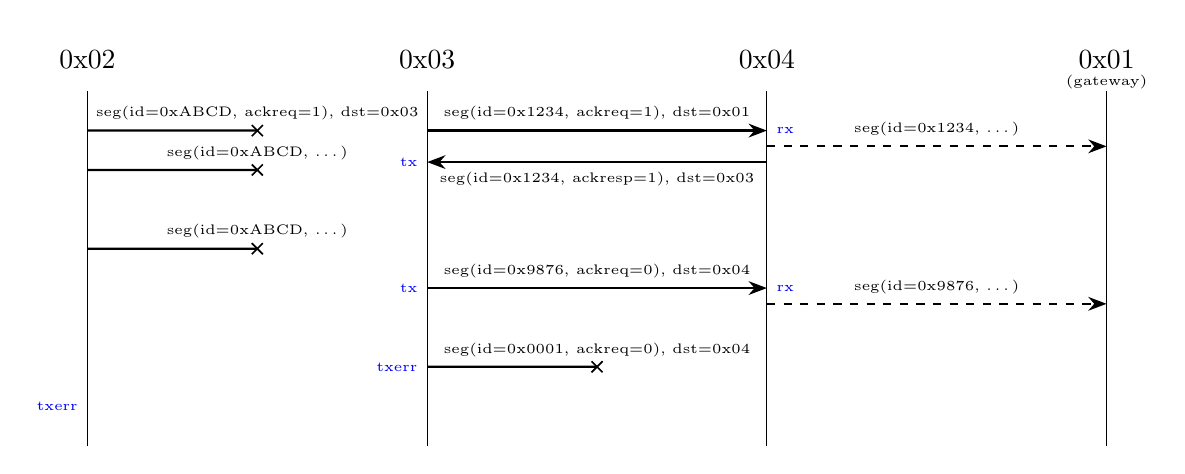
\begin{tikzpicture}[
        device/.style={draw=none, minimum width=1cm, minimum height=0.8cm},
        msg/.style={-Stealth, thick},
        wan/.style={-Stealth, thick, dashed},
        timeout/.style={red, thick, dashed},
        node distance=3.3cm,
        timeline/.style={draw, dashed, white},
        fail/.style={thick, cross at end}
    ]
    
    % Devices
    \node[device] (dev1) at (0,0) {\fitx{0x02}};
    \node[device, right=of dev1] (dev2) {\fitx{0x03}};
    \node[device, right=of dev2] (dev3) {\fitx{0x04}};
    \node[device, right=of dev3] (gw) {\fitx{0x01}};

    \node[above] at ($(gw.south)+(0,-0.1)$) {\tiny(\est{gateway})};

    \draw ($(dev1.south) + (0,0)$) -- ($(dev1.south) + (0,-4.5)$);
    \draw ($(dev2.south) + (0,0)$) -- ($(dev2.south) + (0,-4.5)$);
    \draw ($(gw.south) + (0,0)$) -- ($(gw.south) + (0,-4.5)$);
    \draw ($(dev3.south) + (0,0)$) -- ($(dev3.south) + (0,-4.5)$);

    \draw[msg] ($(dev2.south)+(0,-0.5)$) -- ($(dev3.south)+(0,-0.5)$) node[midway, above] {\tiny{seg(id=\fitx{0x1234}, ackreq=\fitx{1}), dst=\fitx{0x01}}};
    \draw[wan] ($(dev3.south)+(0,-0.7)$) -- ($(gw.south)+(0,-0.7)$) node[midway, above] {\tiny{seg(id=\fitx{0x1234}, \dots)}};
    \draw[msg] ($(dev3.south)+(0,-0.9)$) -- ($(dev2.south)+(0,-0.9)$) node[midway, below] {\tiny{seg(id=\fitx{0x1234}, ackresp=\fitx{1}), dst=\fitx{0x03}}};
    \draw[blue] ($(dev2.south)+(0,-0.9)$) node[left] {\tiny{\acro{tx}}};
    \draw[blue] ($(dev3.south)+(0,-0.5)$) node[right] {\tiny{\acro{rx}}};
    
    \draw[fail] ($(dev1.south)+(0,-0.5)$) -- ($ (dev1.south) !0.5! (dev2.south) + (0, -0.5)$) node[above] {\tiny{seg(id=\fitx{0xABCD}, ackreq=\fitx{1}}), dst=\fitx{0x03}};
    \draw[fail] ($(dev1.south)+(0,-1)$) -- ($ (dev1.south) !0.5! (dev2.south) + (0, -1)$) node[above] {\tiny{seg(id=\fitx{0xABCD}, \dots)}};
    \draw[fail] ($(dev1.south)+(0,-2)$) -- ($ (dev1.south) !0.5! (dev2.south) + (0, -2)$) node[above] {\tiny{seg(id=\fitx{0xABCD}, \dots)}};
    % \draw[fail] ($(dev1.south)+(0,-4)$) -- ($ (dev1.south) !0.5! (dev2.south) + (0, -4)$) node[above] {\tiny{seg(id=\fitx{0xABCD}, \dots)}};
    \draw[blue] ($(dev1.south)+(0,-4)$) node[left] {\tiny{\acro{txerr}}};

    \draw[msg] ($(dev2.south)+(0,-2.5)$) -- ($(dev3.south)+(0,-2.5)$) node[midway, above] {\tiny{seg(id=\fitx{0x9876}, ackreq=\fitx{0}), dst=\fitx{0x04}}};
    \draw[wan] ($(dev3.south)+(0,-2.7)$) -- ($(gw.south)+(0,-2.7)$) node[midway, above] {\tiny{seg(id=\fitx{0x9876}, \dots)}};
    \draw[blue] ($(dev2.south)+(0,-2.5)$) node[left] {\tiny{\acro{tx}}};
    \draw[blue] ($(dev3.south)+(0,-2.5)$) node[right] {\tiny{\acro{rx}}};

    \draw[fail] ($(dev2.south)+(0,-3.5)$) -- ($ (dev2.south) !0.5! (dev3.south) + (0, -3.5)$) node[above] {\tiny{seg(id=\fitx{0x0001}, ackreq=\fitx{0}), dst=\fitx{0x04}}};
    \draw[blue] ($(dev2.south)+(0,-3.5)$) node[left] {\tiny{\acro{txerr}}};

    \end{tikzpicture}
    \caption{Exemple de comunicació entre }
    \label{fig:transport_exemple_1}
\end{figure}

\subsection{Capa d'aplicació}
La capa d'aplicació és la més alta del protocol, i s'encarrega de gestionar les aplicacions que l'utilitzen. Tot i que no forma part del protocol, actua com a interfície entre aquest i les aplicacions, permetent que cada aplicació pugui definir i implementar la seva pròpia capa d'aplicació de manera independent, sense interferir amb la resta. 

En ser independent, poden coexistir múltiples aplicacions, on cadascuna defineix la seva pròpia estructura de dades. Tal com s'ha vist en la capa de transport, cada aplicació s'identifica mitjançant un port, que ha de ser únic. Gràcies a la implementació de la capa de transport, les aplicacions només són notificades dels missatges que els corresponen, de manera que no cal que cada una filtri els missatges rebuts.

Així, el desenvolupament de la capa d'aplicació és una tasca de l'usuari final, i dependrà completament dels requisits i característiques específiques de cada cas. A continuació s'indiquen, com a exemple, alguns protocols de capa d'aplicació que podrien existir:
\begin{itemize}
    \item \emph{Configuració dinàmica}. Permet modificar paràmetres del protocol durant el seu funcionament, com ara la potència de transmissió, el nombre d'intents de retransmissió o el temps d'espera per a la recepció dels \acro{ack} de la capa d'accés al medi.
    \item \emph{Gestió de la xarxa}. Ofereix la possibilitat d'afegir o eliminar nodes i, per tant, de modificar les taules de rutes dels dispositius.
    \item \emph{Baix consum}. Gestiona els modes de baix consum dels nodes, proporcionant mecanismes de sincronització amb la resta de dispositius per evitar la pèrdua de funcionalitat d'encaminament.
\end{itemize}

Al \autoref{chap:adaptacio_baix_consum} es detalla la implementació de l'últim exemple, definint la situació d'ús i els mecanismes utilitzats.

\section{Proves i validació del protocol}
Per tal de verificar el correcte funcionament del protocol, s'han desenvolupat fitxers de prova específics per a cada capa. Aquests fitxers implementen una situació de comunicació coneguda on el comportament del protocol és previsible, i permeten verificar-ne el seu correcte funcionament. Part d'aquestes situacions controlades s'han basat en els diagrames d'exemple exposats anteriorment. Aquests fitxers de prova són útils també com a exemple d'ús del protocol, i poden servir com a base per a nous protocols de cada capa. Es poden consultar a la ruta \fitx{firmware/exemples}.

La implementació del protocol inclou traces de depuració, distingides entre informació, avís, i error, amb les quals és possible conèixer l'estat del protocol en cada moment. 

Les proves s'han realitzat de forma manual, observant l'estat del sistema a través de les traces, i verificant el comportament del protocol a través dels diagrames de funcionament previst. Part de les proves han requerit d'intervenció manual, com ara la desconnexió de dispositius (per simular-ne una fallada), o la programació d'enviaments de \est{downlinks} a través de \acro{ttn}.

Una clara limitació ha estat la manca de dispositius. A causa de només disposar d'un \est{gateway} i de dos dispositius, no s'ha pogut verifica el funcionament del protocol en grans xarxes, o en topologies complexes. 

% // TODO: Verificació de distància?

% // TODO: Posar aquí un exemple de log de comunicació?

En el procés de validació es van observar inconsistències en el funcionament del protocol. Les més rellevants, que impedien el funcionament total del protocol, són les següents:
\begin{itemize}
    \item Els temps d'espera de recepció d'\acro{ack} no eren coherents, i resultaven en \est{timeouts} prematurs. Això es devia a iniciar el temporitzador de recepció d'\acro{ack} quan s'iniciava la transmissió, i no en la seva finalització.
    \item Després de realitzar una verificació de l'estat del canal (a través de \acro{cad}), en transductor no es posava, de forma automàtica, en estat de recepció. Això provocava que no es produís la interrupció de recepció i, per tant, que no es processessin els missatges rebuts.
    \item Configuració de la ràdio en LoRaWAN i LoRa. Després de realitzar una transmissió a través de LoRaWAN, no es rebien missatges enviats a través de LoRa. Això es devia a que la ràdio quedava amb la configuració de LoRaWAN, i no es tornava a configurar per a LoRa. Es va solucionar a través de la capa d'abstracció \est{LoRa}, superior a \est{LoRaWAN} i {LoRaRAW}.
\end{itemize}

Després de les verificacions, cada capa del protocol verifica els requisits prèviament definits, amb la fiabilitat i el baix consum de les transmissions com a objectius principals. Tot i que no s'han pogut realitzar proves en entorns reals i topologies més complexes, es considera que el protocol estableix una base funcional i estable per a la seva aplicació.

\chapter{Adaptació a entorns de baix consum}
\label{chap:adaptacio_baix_consum}
En el desenvolupament del protocol, s'ha posat èmfasi en la reducció del consum energètic. En xarxes de monitoratge, com ara les agrícoles o ferroviàries, el subministrament energètic dels dispositius pot no estar garantit, i una mala gestió del consum pot resultar en temps d'ús molt reduïts.

Una característica de les comunicacions és que el receptor no coneix quan un transmissor enviarà un missatge. Això provoca que el receptor hagi d'estar, sempre que ell no vulgui transmetre, en estat de recepció, fent impossible aplicar modes de baix consum.

En aquest capítol es presenta, primerament, les limitacions del protocol implementat sense optimitzacions energètiques addicionals. Seguidament, es presenten les estratègies considerades, basades en la sincronització entre nodes per permetre modes de baix consum, i implementades a la capa d'aplicació. Finalment, es presenten les proves realitzades per verificar el correcte funcionament de la solució, i els seus resultats i limitacions.

\section{Descripció de l'escenari: xarxa lineal de sensors}
L'adaptació s'ha realitzat en un entorn concret i conegut, aprofitant les característiques de la xarxa per implementar i optimitzar la solució. Aquest fet permet que la solució sigui eficient en aquest context, però no garanteix que pugui ser aplicable en altres topologies. 

L'escenari considerat és una xarxa lineal de dispositius, amb connectivitat a un \est{gateway} LoRaWAN a través d'un dels seus extrems. Per simplicitat, es considera també que cada dispositiu es pot comunicar únicament amb els dos veïns immediats. Això es pot assegurar mitjançant les taules d'encaminament, definint les rutes per tal que cada dispositiu utilitzi únicament els seus veïns. 

\begin{figure}
    \centering
    \includegraphics[width=0.95\linewidth]{imatges/situacioBaixConsum.drawio.pdf}
    \caption{Representació de la topologia considerada per a l'adaptació del protocol.}
    \label{fig:topologia_baix_consum}
\end{figure}

Aquesta topologia pot ser útil en entorns agrícoles, on els sensors es poden co\l.locar al llarg d'una línia de cultiu, o en entorns ferroviaris, on els sensors es poden trobar al llarg de les vies. 

També s'ha limitat el comportament i les funcionalitats del protocol:
\begin{enumerate}
    \item La comunicació és, únicament, unidireccional. És a dir, els nodes únicament envien dades, i no esperen rebre'n. Aquesta consideració és deguda a que en aplicacions de monitoratge és poc freqüent voler enviar dades cap a un dispositiu de lectura.
    \item Cada dispositiu vol enviar únicament un missatge, amb destí al \est{gateway}. En un cicle de funcionament del dispositiu, aquest envia la lectura de les seves dades al \est{gateway} el qual, si es vol, les farà arribar a un servidor d'aplicació d'internet per a processar-les.
    \item Els dispositius coneixen l'interval de temps entre transmissions ---la durada d'un cicle de funcionament---. Un cop transcorregut aquest temps, el dispositiu inicia una nova transmissió de la seva lectura cap al \est{gateway}.
\end{enumerate}

A la \autoref{fig:topologia_baix_consum} es pot veure representada la situació exposada, on el dispositiu \fitx{D4} és l'únic dispositiu amb capacitats LoRaWAN.

A més, es vol garantir en la mesura del possible la fiabilitat a llarg termini. És a dir, es prefereix que l'aplicació funcioni incorrectament durant un període de temps curt, i que després es recuperi, a que la comunicació sigui fiable durant un període de temps més llarg, però deixi de funcionar permanent després d'un error. És una característica important, sobretot en dispositius on no es pot garantir l'alimentació: si un dispositiu s'atura, és millor que després pugui recuperar les seves funcionalitats automàticament, que no pas que es quedi aturat indefinidament.


\section{Limitacions del protocol sense optimitzacions energètiques}
Malgrat haver realitzat el disseny del protocol considerant el consum energètic, les optimitzacions realitzades no són suficients per fer-lo viable en entorns on el consum energètic és crític. Això és degut a que tots els dispositius han de trobar-se sempre en estat de recepció, per poder fer d'encaminadors d'altres dispositius. A causa d'això, existeix un consum energètic constant, que malgrat ser reduït, no és assumible per a dispositius que no disposen de subministrament energètic constant.

Per posar-ho en context, s'ha observat de forma experimental com el consum de la placa de desenvolupament (que inclou el microcontrolador, reguladors de tensió, etc.) i de la ràdio en estat de recepció és, aproximadament, de \SI{75}{\milli\ampere}. Així, si considerem un dispositiu amb una bateria de \SI{2500}{\milli\ampere\hour}, una capacitat estàndard per bateries de mida física reduïda, el temps màxim d'ús del dispositiu és de 33.33 hores, poc més d'un dia.

Podríem obtenir valors més optimistes si considerem únicament el consum del microcontrolador i de la ràdio, tenint en compte que es podrien utilitzar reguladors de tensió i perifèrics més eficients. A partir de dades de \cite{espressif_current_nodate}, s'obté que el microcontrolador consumeix, de forma activa, aproximadament \SI{20}{\milli\ampere}, i de \cite{semtech_sx1262_nodate} que el consum mínim de la ràdio en recepció és de \SI{5}{\milli\ampere}. Així, el consum total seria aproximadament de \SI{25}{\milli\ampere}, amb un temps màxim d'ús de 100 hores, poc més de 4 dies.

S'observa com ni en el cas més optimista s'aconsegueix una temps de funcionament prolongat, fent que l'ús d'aquest protocol impliqués substitucions de bateries de forma regular, o bé l'ús de dispositius externs (com ara panells solars) per augmentar el temps de funcionament. 

\section{Estratègies de sincronització}
\label{section:estrategiesSync}
Per tal de reduir el consum, podem tenir en compte les consideracions 1 i 2, que limiten el comportament dels dispositius a una única transmissió per cicle, i que no esperen ser receptors de cap missatge. 

Podem dividir el cicle de funcionament dels dispositius en dues parts:
\begin{enumerate}
    \item \emph{Baix consum}. És el temps on els dispositius es troben en mode de baix consum, i no realitzen cap altra funció. En aquest estat la ràdio no funciona, i per tant no poden realitzar cap funció d'encaminament.
    \item \emph{Funcionament normal}. És el temps on els dispositius es troben actius, realitzen la seva lectura, generen el missatge de transmissió, i actuen com a encaminadors d'altres dispositius ---en aquest cas, únicament del dispositiu anterior a aquest---. 
\end{enumerate}

En el període de funcionament, és important que els dispositius es trobin actius i en mode de recepció, per mantenir les funcionalitats d'encaminament. Per tal d'aconseguir-ho, els dispositius han de trobar-se sincronitzats, fent que es trobin en el mateix estat de funcionament al mateix temps. Això es pot aconseguir, principalment, mitjançant dues estratègies:
\begin{enumerate}
    \item \emph{Rellotge intern}. Cada dispositiu disposa d'un rellotge intern que li permet determinar la durada dels períodes de baix consum i de funcionament. Establint el mateix cicle en tots els dispositius, i iniciant-los simultàniament, s'aconsegueix mantenir-los sincronitzats. Malgrat ser una solució senzilla d'implementar, presenta una limitació important: l'error del rellotge. Aquest error s'acumula amb el pas del temps, fent que els dispositius s'acabin desincronitzant.
    
    Tot i que l'error podria semblar insignificant, s'ha observat que el rellotge utilitzat en mode de baix consum pot tenir desviacions superiors a 5000 parts per millió (\emph{ppm}), equivalents de més de set minuts per dia de funcionament \cite{nikki_smith_esp32_2022}. A més, aquest error depèn també de la temperatura, fent-lo imprevisible. Malgrat existir mecanismes per reduir aquest error, com ara utilitzar osci\l.ladors externs, l'error no és mai nul, i s'acaba acumulant mb el temps, desincronitzant els dispositius.
    
    \item \emph{Sincronització externa}. Es basa en un mecanisme de sincronització entre dispositius, on un dels dispositius actua com a referència, i la resta s'ajusten a aquest. Això es pot aconseguir mitjançant un missatge de sincronització generat per aquest dispositiu, el qual, en rebre's, indica l'inici del cicle de funcionament durant una període conegut i igual per a cada dispositiu. Aquest missatge es trobaria a nivell d'aplicació. 
    
    Malgrat seguir utilitzant el rellotge intern per regular el temps de baix consum i funcionament, la sincronització amb el dispositiu de referència permet corregir l'error acumulat. 
    Continua sent important que els dispositius es trobin actius abans de rebre el missatge de sincronització; en cas contrari, no existeix sincronització i, per tant, no es corregeix l'error que ha introduït el rellotge intern.
\end{enumerate}

Per tal de garantir la fiabilitat a llarg termini, i evitar la desincronització amb el pas del temps, s'ha optat per utilitzar el mecanisme de sincronització externa. 

Per aconseguir que tots els dispositius es puguin sincronitzar, és important que cada dispositiu propagui aquest missatge al següent dispositiu (o dispositius). Així, quan l'aplicació, que d'ara endavant es denominarà \emph{aplicació de baix consum}, rebi un missatge de sincronització, el propagarà al següent dispositiu, del qual n'ha de conèixer l'adreça. Aquesta opció és més òptima que no pas fer que sigui el dispositiu de referència qui genera un missatge de sincronització per a cada dispositiu, ja que aquesta opció implicaria moltes més transmissions ($\sum_{x=0}^{D-1}{x}$, on \emph{D} és el nombre de dispositius), en vers a una única transmissió per cada dispositiu diferent del de referència ($D-1$ transmissions). A causa d'aquest major nombre de missatges de sincronització, el temps necessari per tenir tots els dispositius sincronitzats és també més llarg. A la \autoref{fig:app_opcionsIniciSync} es representen ambdues opcions.

\begin{figure}
    \centering
    \includegraphics[width=0.95\linewidth]{imatges/opcionsQuiEnviaSync.drawio.pdf}
    \caption{Propagació del missatge de sincronització. A l'esquerra, el missatge de sincronització és enviat pel dispositiu de referència. A la dreta, el missatge de sincronització és propagat per cada dispositiu.}
\label{fig:app_opcionsIniciSync}
\end{figure}

En els següents apartats es presenten els diferents mecanismes de sincronització externa considerats, amb les seves diferències i limitacions.
% PARLAR DE SINCRONITZACIÓ INICIAL

\section{Sincronització explícita}
Com a sincronització explícita es considera l'ús d'un missatge especial i fàcilment identificable. Com s'ha comentat, el propòsit d'aquest missatge és indicar l'instant d'inici de cicle de funcionament normal, i eliminar l'error introduït pel rellotge intern. En aquest apartat es mostren dues estratègies considerades, on la diferència principal entre aquestes és el moment de transmissió de les dades.

\subsection{Dades transmeses després de la sincronització}
Quan un dispositiu inicia el mode de funcionament normal, espera rebre un missatge de sincronització. En el moment que el rep, inicia el seu cicle de funcionament, i propaga el missatge al següent dispositiu. Després d'això, pot realitzar la seva lectura, i generar la transmissió de les dades. Gràcies a que prèviament havia propagat el missatge de sincronització, qualsevol dels seus dos veïns immediats es troben sincronitzats ---bé perquè és qui li ha enviat el missatge, o és a qui li ha propagat---, i per tant poden actuar com a encaminadors.

El funcionament canvia quan el dispositiu és el de referència. En aquest cas, l'inici del cicle de funcionament comença immediatament, generant i transmetent el missatge de sincronització. A continuació pot fer la seva lectura, i transmetre-la com qualsevol altre node.

Aquest plantejament introdueix un fet important: el dispositiu de referència ha de despertar del mode de baix consum més tard que els dispositius a qui ha d'enviar el missatge de sincronització, ja que si no aquests no el rebrien. Aquest temps ha de ser, com a mínim, igual al temps de transmissió del missatge de sincronització. Una solució fàcil per aconseguir-ho és restant aquest temps del de baix consum, de manera que despertarà abans. 

A la \autoref{fig:app_opcioSyncExp1} es representa aquest comportament. El dispositiu de referència és \fitx{D1} (ressaltat en negreta), i el dispositiu amb capacitats LoRaWAN és el \fitx{D4} (ressaltat en verd). Les dades es transmeten en direcció al \est{gateway}, creuant els dispositius intermedis fins a arribar a \fitx{D4}. Es representen els missatges de sincronització com a \fitx{TX_S}, i els de dades com a \fitx{TX_Dn}, on \fitx{n} indica l'origen de les dades. Les recepcions respectives d'aquests missatges s'identifiquen amb el prefix \fitx{RX}. S'indica també quan cada dispositiu desperta i inicia el mode de baix consum, amb línies verdes i vermelles respectivament, i amb el període de baix consum ressaltat en vermell clar. L'eix horitzontal es correspon al temps, i el vertical als dispositius, que es podria entendre com una distància.

Per simplicitat i per evitar sobrecarregar el diagrama, només s'han representat les recepcions dels missatges en el dispositiu destinatari; per exemple, per al missatge \fitx{TX_S} enviat per \fitx{D2}, només es mostra la recepció a \fitx{D3}, tot i que \fitx{D1} també el rebria. No obstant això, com que no és el destinatari final, l'ignoraria. A més, cal tenir en compte que cada transmissió representa una transmissió de la capa d'accés al medi, i per tant inclou també una part de recepció per rebre el reconeixement.

S'observa com el la durada del cicle és de vuit unitats de temps, sent dues d'aquestes destinades al funcionament normal (després de rebre i propagar la sincronització). Es mostra com els dispositiu que no són el de referència es troben fora del mode de baix consum durant una unitat de temps més: és així ja que en aquesta reben la sincronització.

% « »

\begin{figure}
    \centering
    \setlength{\extrarowheight}{0pt}
    \addtolength{\extrarowheight}{\aboverulesep}
    \addtolength{\extrarowheight}{\belowrulesep}
    \setlength{\aboverulesep}{0pt}
    \setlength{\belowrulesep}{0pt}
    \arrayrulecolor{black}
    \resizebox{\linewidth}{!}{%
        \begin{tabular}{
            !{\vrule width \heavyrulewidth}c!{\vrule width \heavyrulewidth}c!{\color[rgb]{0.451,0.804,0.443}\vrule width \heavyrulewidth}c|c|c|c|cccc!{\color[rgb]{0.451,0.804,0.443}\vrule width \heavyrulewidth}c|c!{\vrule width \heavyrulewidth}}             
            \toprule
        \textbf{D1} & {\cellcolor[rgb]{1,0.847,0.808}} & TX\_S & TX\_D1 & \multicolumn{1}{c!{\color[rgb]{1,0.349,0.349}\vrule width \heavyrulewidth}}{} & \multicolumn{1}{c}{{\cellcolor[rgb]{1,0.847,0.808}}} & {\cellcolor[rgb]{1,0.847,0.808}} & {\cellcolor[rgb]{1,0.847,0.808}}~~~~~~~~~~~ & {\cellcolor[rgb]{1,0.847,0.808}}~~~~~~~~~~~ & {\cellcolor[rgb]{1,0.847,0.808}}~~~~~~~~~~~ & TX\_S &  \\ \hhline{~>{\arrayrulecolor[rgb]{1,0.847,0.808}}->{\arrayrulecolor{black}}---~>{\arrayrulecolor[rgb]{1,0.847,0.808}}---->{\arrayrulecolor{black}}-~}
        D2 & {\cellcolor[rgb]{1,0.847,0.808}} & RX\_S & TX\_S & TX\_D2 & \multicolumn{1}{c!{\color[rgb]{1,0.349,0.349}\vrule width \heavyrulewidth}}{} & {\cellcolor[rgb]{1,0.847,0.808}} & {\cellcolor[rgb]{1,0.847,0.808}} & {\cellcolor[rgb]{1,0.847,0.808}} & {\cellcolor[rgb]{1,0.847,0.808}} & RX\_S & … \\ \hhline{~>{\arrayrulecolor[rgb]{1,0.847,0.808}}->{\arrayrulecolor{black}}----~>{\arrayrulecolor[rgb]{1,0.847,0.808}}--->{\arrayrulecolor{black}}-~}
        D3 & \multicolumn{1}{c}{{\cellcolor[rgb]{1,0.847,0.808}}} & \multicolumn{1}{c!{\color[rgb]{0.451,0.804,0.443}\vrule width \heavyrulewidth}}{{\cellcolor[rgb]{1,0.847,0.808}}} & RX\_S & TX\_S & TX\_D3 & \multicolumn{1}{c!{\color[rgb]{1,0.349,0.349}\vrule width \heavyrulewidth}}{~~~~~~~~~~~ } & {\cellcolor[rgb]{1,0.847,0.808}} & {\cellcolor[rgb]{1,0.847,0.808}} & \multicolumn{1}{c}{{\cellcolor[rgb]{1,0.847,0.808}}} & \multicolumn{1}{c!{\color[rgb]{0.451,0.804,0.443}\vrule width \heavyrulewidth}}{{\cellcolor[rgb]{1,0.847,0.808}}} &  \\ \hhline{~>{\arrayrulecolor[rgb]{1,0.847,0.808}}-->{\arrayrulecolor{black}}----~>{\arrayrulecolor[rgb]{1,0.847,0.808}}----}
        \textbf{\textcolor[rgb]{0,0.502,0}{D4}} & \multicolumn{1}{c}{{\cellcolor[rgb]{1,0.847,0.808}}~~~~~~~~~~~} & \multicolumn{1}{c}{{\cellcolor[rgb]{1,0.847,0.808}}~~~~~~~~~~~} & \multicolumn{1}{c!{\color[rgb]{0.451,0.804,0.443}\vrule width \heavyrulewidth}}{{\cellcolor[rgb]{1,0.847,0.808}}~~~~~~~~~~~} & RX\_S & TX\_S & \multicolumn{1}{c|}{TX\_D4} & \multicolumn{1}{c!{\color[rgb]{1,0.349,0.349}\vrule width \heavyrulewidth}}{} & {\cellcolor[rgb]{1,0.847,0.808}} & \multicolumn{1}{c}{{\cellcolor[rgb]{1,0.847,0.808}}} & \multicolumn{1}{c}{{\cellcolor[rgb]{1,0.847,0.808}}~~~~~~~~~~~} & {\cellcolor[rgb]{1,0.847,0.808}}~~~~~~~~~~~ \\ \arrayrulecolor{black}\toprule
    \multicolumn{1}{c}{\est{gateway}} & \multicolumn{11}{c}{} \\

        \end{tabular}
    }
    \caption{Transmissió de dades després de sincronització.}
    \label{fig:app_opcioSyncExp1}
\end{figure}

Aquest mecanisme podria semblar correcte, però s'observen problemes quan es considera un fet mencionat anteriorment: el dispositiu veí que no és receptor també rep els missatges transmesos, provocant co\l.lisions. Per exemple, la transmissió de les dades de \fitx{D1} coincideix amb el missatge de sincronització enviat per \fitx{D2} a \fitx{D3}. En aquest moment \fitx{D2} es posa en recepció momentàniament per obtenir l'\acro{ack} de \fitx{D3}, però també rep la transmissió de \fitx{D1}. Això fa que cap de les dues transmissions sigui satisfactòria.

Per tant, aquest mecanisme no és viable si dos nodes veïns transmeten alhora, fent que les  les co\l.lisions siguin inevitables.
Es vol destacar que el diagrama no està complet ni representa totes les transmissions, sinó que únicament s'han mostrat les necessàries per trobar la primera co\l.lisió. 

\subsection{Dades transmeses en blocs}
Una segona opció consisteix en dividir les transmissions de dades en dos blocs: en el primer bloc transmeten els dispositius en posició senar (\fitx{D1, D3}, etc.), i en el segon bloc els dispositius en posició parell (\fitx{D2, D4}, etc.). Per si sol això no és suficient, ja que dos veïns continuen transmetent simultàniament quan un envia el missatge de sincronització i l'altre les dades. Per evitar-ho, es pot aplicar un marge abans de transmetre les dades, de com a mínim el temps de transmissió del missatge de sincronització. 

En aquest escenari és necessari també que el dispositiu de referència sigui el que té capacitats LoRaWAN. Això permet que els nodes més propers al \est{gateway} siguin els primers a transmetre les seves dades. En cas que la referència fos el dispositiu més allunyat (com en l'exemple anterior), els primers a transmetre haurien d'enviar les dades al node que s'acaba de sincronitzar. Això pot generar problemes, ja que si el dispositiu es troba en el primer bloc de transmissió, també voldrà enviar les seves dades i, a més, haurà d'encaminar les dades anteriors. Aquest fet s'accentua com més proper es el dispositiu al \est{gateway}, ja que ha de realitzar molts més encaminaments.

Aquesta segona opció, tot i reduir el risc de co\l.lisions, afegeix major complexitat, sent necessari determinar quan el segon bloc de dispositius poden iniciar les seves transmissions:
\begin{itemize}
    \item \emph{Temps aleatori}. Els dispositius del segon bloc esperen un temps aleatori després de propagar el missatge de sincronització. El més senzill d'implementar, però no garenteix que la transmissió no es realitzi en el bloc de transmissions senar, i és totalment imprevisible.
    \item \emph{Temps fix}. Esperen un temps preestablert després de propagar el missatge de sincronització. Aquest temps hauria de ser suficientment gran com per permetre que totes les transmissions dels nodes senars anteriors a aquest s'hagin realitzat. En cas contrari, iniciaria la seva transmissió en el bloc de temps incorrecte, provocant co\l.lisions.
\end{itemize}


En qualsevol dels dos casos, aquesta solució implica una coordinació temporal molt més precisa, ja que cal definir per a cada node quan ha de transmetre i quan pot tornar al mode de baix consum. El funcionament resultant s'assembla molt a un esquema de \acro{tdma} (Time Division Multiple Access), on cada dispositiu disposa d'un interval de temps específic per accedir al canal.

A la \autoref{fig:app_opcioSyncExp2} es representa aquest comportament, on cal recordar que \fitx{D1} ara és qui té capacitats LoRaWAN i també actua com a referència. El diagrama no representa totes les transmissions, ja que això el faria massa complex i complicat de llegir; per aquest motiu es representen únicament les del bloc senar, i les inicials del bloc parell.

\begin{figure}
    \centering
\setlength{\extrarowheight}{0pt}
\addtolength{\extrarowheight}{\aboverulesep}
\addtolength{\extrarowheight}{\belowrulesep}
\setlength{\aboverulesep}{0pt}
\setlength{\belowrulesep}{0pt}
\arrayrulecolor{black}
\resizebox{\linewidth}{!}{%
\begin{tabular}{!{\vrule width \heavyrulewidth}c!{\vrule width \heavyrulewidth}c!{\color[rgb]{0.451,0.804,0.443}\vrule width \heavyrulewidth}c|c|c|c|c|c|cc|c|c!{\vrule width \heavyrulewidth}} 
    \multicolumn{1}{c}{\est{gateway}} & \multicolumn{11}{c}{} \\
    \toprule
\textbf{\textcolor[rgb]{0,0.502,0}{D1}} & {\cellcolor[rgb]{1,0.847,0.808}} & TX\_S & \tiny marge & TX\_D1 & \multicolumn{1}{c}{} &  & RX\_D3 & \multicolumn{1}{c|}{TX\_D3} & ~~~~~~~~~~~ & RX\_D2 & TX\_D2 \\ 
\hhline{~>{\arrayrulecolor[rgb]{1,0.847,0.808}}->{\arrayrulecolor{black}}---~---~--}
D2 & {\cellcolor[rgb]{1,0.847,0.808}} & RX\_S & TX\_S & \multicolumn{1}{c}{} &  & RX\_D3 & TX\_D3 &  &  & TX\_D2 &  \\ 
\hhline{~>{\arrayrulecolor[rgb]{1,0.847,0.808}}->{\arrayrulecolor{black}}---~--~~--}
D3 & \multicolumn{1}{c}{{\cellcolor[rgb]{1,0.847,0.808}}} & \multicolumn{1}{c!{\color[rgb]{0.451,0.804,0.443}\vrule width \heavyrulewidth}}{{\cellcolor[rgb]{1,0.847,0.808}}} & RX\_S & TX\_S & \tiny marge & TX\_D3 & \multicolumn{1}{c}{} &  & \multicolumn{1}{c}{} &  & RX\_D4 \\ 
\hhline{~>{\arrayrulecolor[rgb]{1,0.847,0.808}}-->{\arrayrulecolor{black}}----~~~~-}
D4 & \multicolumn{1}{c}{{\cellcolor[rgb]{1,0.847,0.808}}~~~~~~~~~~} & \multicolumn{1}{c}{{\cellcolor[rgb]{1,0.847,0.808}}~~~~~~~~~~} & \multicolumn{1}{c!{\color[rgb]{0.451,0.804,0.443}\vrule width \heavyrulewidth}}{{\cellcolor[rgb]{1,0.847,0.808}}~~~~~~~~~~} & RX\_S & TX\_S & \multicolumn{1}{c}{} & \multicolumn{1}{c}{} &  & \multicolumn{1}{c}{} &  & TX\_D4 \\ 
\toprule
\multicolumn{1}{l}{} & \multicolumn{1}{l}{} & \multicolumn{1}{l}{} & \multicolumn{1}{c!{\color[rgb]{0.753,0.753,0.753}\vrule width \heavyrulewidth}}{} & \multicolumn{5}{c!{\color[rgb]{0.753,0.753,0.753}\vrule width \heavyrulewidth}}{\textcolor[rgb]{0.753,0.753,0.753}{Bloc senar}} & \multicolumn{1}{l!{\color[rgb]{0.753,0.753,0.753}\vrule width \heavyrulewidth}}{} & \multicolumn{2}{c}{\textcolor[rgb]{0.753,0.753,0.753}{Bloc parell...}}
\end{tabular}
}
    \caption{Transmissió de dades en blocs senars/parells.}
    \label{fig:app_opcioSyncExp2}
\end{figure}

S'observa com, gràcies a que cada dispositiu té «assignat» els seu instant de temps per fer la seva transmissió, i gràcies al marge de després de propagar la sincronització, s'eviten les co\l.lisions tant entre dades, com entre dades i sincronització. Tot i això, aquesta solució no és viable, pels motius següents:
\begin{enumerate}
    \item Cada dispositiu ha de seguir un comportament específic i diferent, amb instants de transmissió i d'inici de baix consum diferents. Això complica la implementació i el manteniment.
    \item La durada del cicle de funcionament normal ---des que surt del mode de baix consum fins que torna a iniciar-lo--- és molt elevat. El node més proper al \est{gateway} ha d'esperar-se a que el node més allunyat realitzi la seva transmissió, i aquesta s'encamini a través de tota la xarxa.  
    \item El nombre de transmissions que realitza cada dispositiu no és homogeni. Els nodes més propers al \est{gateway} en realitzaran més (tantes com nodes anteriors a ell hi hagi). Tenint en compte que les transmissions tenen un consum energètic elevat, fa que el consum tampoc sigui homogeni. Aquest fet comporta més complexitat de manteniment ja que, per exemple, comporta a no poder modificar totes les bateries dels dispositius a la mateixa vegada, ja que no han consumit el mateix. És cert que es pot intentar evitar utilitzant bateries de capacitats diferents, però llavors implicaria també un disseny previ més complex.
    \item No considera la possibilitat que una transmissió pugui fallar, resultant en retransmissions. Una retransmissió es podria superposar a la transmissió de dades d'un altre dispositiu, generant co\l.lisions. A més, si el següent node també podria haver de realitzar una retransmissió per encaminar les dades, agreujant més la situació 
\end{enumerate}

Es va considerar la possibilitat d'utilitzar més de dos blocs, per exemple en múltiples de tres, fet que faria que les transmissions es trobessin més espaïades, reduint la probabilitat de solapaments entre transmissions. Es va descartar la opció, ja que augmentaria encara més la durada del cicle de funcionament normal, i tampoc evitaria les co\l.lisions si es produïssin més retransmissions que l'espai obtingut en afegir aquest nou bloc.

Finalment, es va descartar la implementació de qualsevol de les opcions anteriors, ja que requereixen una quantitat molt elevada de transmissions. Amb \fitx{N} dispositius, el nombre total de transmissions (incloent-hi les dades i missatges de sincronització) és aproximadament $\sum{N} + N$, fet que incrementa el consum energètic i la saturació del canal. A més, la lògica de funcionament és excessivament complexa, dificultant la implementació d'aquesta solució. 

\subsection{Dades acumulades}
Com s'ha comentat, un dels principals inconvenients de les solucions anteriors és l'elevat nombre de transmissions que es realitzen en cada cicle. Això es deu al fet que cada dispositiu genera el seu propi segment de dades amb destí final al gateway. Ja que la topologia és lineal, aquest segment ha de ser encaminat a través dels dispositius intermedis, els quals han de retransmetre'l fins al seu destí, fent que el nombre de transmissions i l'ús del canal creixi de forma exponencial amb el nombre de dispositius. 

Per tal de reduir aquest nombre de transmissions, s'ha optat per acumular les dades de tots els dispositius en un únic missatge. És important recordar que s'havia limitat el comportament dels dispositius a un únic missatge, i amb el mateix destí final, el \est{gateway}. Si no s'haguessin près aquestes limitacions, aquesta estratègia no seria possible.

El funcionament d'aquest mecanisme és el següent:
\begin{enumerate}
    \item \emph{Sincronització}. El dispositiu de referència continua enviant el missatge de sincronització en sortir del mode de baix consum. El següent dispositiu rep la sincronització, i el propaga al següent. Es continua aplicant el marge d'inici de funcionament normal pels dispositius que no són el de referència, per tal de garantir que reben el missatge de sincronització i que no estan en mode de baix consum quan s'envia.
    \item \emph{Dades}. El dispositiu de l'extrem més llunyà al \est{gateway} envia les seves dades després de rebre el missatge de sincronització. La resta de dispositius, després de propagar la sincronització, queden a l'espera de rebre el missatge de dades. Quan el reben, hi afegeixen les seves dades, i el transmeten al següent dispositiu. S'observa com la propagació del missatge de sincronització i del de dades es realitza en sentits contraris.
    
    Establir un altre dispositiu per enviar primer les dades és incoherent, ja que implicaria que hauria de transmetre les seves dades en sentit contrari al \est{gateway}, les quals després haurien de ser encaminades en sentit contrari.

    \item \emph{Timeout}. Si després d'un temps determinat un dispositiu no ha rebut el missatge de dades, considera que hi ha hagut un error, i inicia ell l'enviament de dades. És important que aquest temps sigui superior en els dispositius més propers al de referència, ja que són els que reben abans el missatge de sincronització i, a més, són qui més tard reben el missatge de dades. En cas contrari, un dispositiu podria generar aquest \est{timeout} quan encara s'estan transmetent les dades, sense que hi hagi hagut cap error. 

    Aquest mecanisme és important, ja que evita perdre les dades de tots els dispositius si un falla. A més, afegeix un mecanisme de detecció d'errors: si existeixen 10 dispositius però només rebem 5 valors de dades, podem assegurar que, com a mínim, hi ha hagut un error en la transmissió entre els dispositius 6 i 5. Si no hi hagués hagut aquest error, el dispositiu 5 hauria rebut les dades del dispositiu 6, hi hauria afegit les seves i, per tant, hauríem rebut com a mínim 6 valors de dades.
    \item \emph{Baix consum}. Després de realitzar la transmissió de les dades, el dispositiu pot tornar al mode de baix consum automàticament. Això és possible gràcies a la consideració que únicament realitzen una transmissió per cicle.
\end{enumerate}


% Explicar qui és referència i qui dades
Una qüestió important és determinar quin dispositiu és el de referència. Inicialment es va considerar utilitzar el dispositiu més proper al \est{gateway}, de manera que la sincronització es propagaria en un únic sentit (des del \est{gateway} cap a l'extrem de la xarxa), mentre que les dades circularien en sentit contrari. Aquesta situació es mostra a la \autoref{fig:app_opcioSyncAcum1}, on el dispositiu \fitx{D1}, el més proper al \est{gateway}, inicia el missatge de sincronització. Per altra banda, el dispositiu \fitx{D6}, situat a l'extrem oposat, és l'encarregat d'iniciar la transmissió de dades després de sincronitzar-se. Les transmissions de dades s'identifiquen com \fitx{TX_Dm:n}, on \fitx{m} representa el dispositiu que ha afegit les primeres dades, i \fitx{n} el dispositiu que ha afegit les últimes.

\begin{figure}[ht]
    \centering
    \setlength{\extrarowheight}{0pt}
    \addtolength{\extrarowheight}{\aboverulesep}
    \addtolength{\extrarowheight}{\belowrulesep}
\setlength{\aboverulesep}{0pt}
\setlength{\belowrulesep}{0pt}
\arrayrulecolor{black}
\resizebox{\linewidth}{!}{%
\begin{tabular}{!{\vrule width \heavyrulewidth}c!{\vrule width \heavyrulewidth}ccccccccccccc!{\vrule width \heavyrulewidth}} 
    \multicolumn{1}{c}{\est{gateway}} & \multicolumn{13}{c}{} \\
\toprule
\textbf{\textcolor[rgb]{0,0.502,0}{D1}} & \multicolumn{1}{c!{\color[rgb]{0.451,0.804,0.443}\vrule width \heavyrulewidth}}{{\cellcolor[rgb]{1,0.847,0.808}}} & \multicolumn{1}{c|}{TX\_S}     &   & ~~~~~~~~~~~~~~ & ~~~~~~~~~~~~~ & ~~~~~~~~~~~~~~ & ~~~~~~~~~~~~~~ & & & \multicolumn{1}{c|}{} & \multicolumn{1}{c|}{RX\_D6:2}  & \multicolumn{1}{c!{\color[rgb]{1,0.349,0.349}\vrule width \heavyrulewidth}}{TX\_D6:1} &       {\cellcolor[rgb]{1,0.847,0.808}}~~~~~~~~~~~~~~          \\ 
\hhline{~>{\arrayrulecolor[rgb]{1,0.847,0.808}}->{\arrayrulecolor{black}}--~~~~~~--->{\arrayrulecolor[rgb]{1,0.847,0.808}}->{\arrayrulecolor{black}}}
{D2} & \multicolumn{1}{c!{\color[rgb]{0.451,0.804,0.443}\vrule width \heavyrulewidth}}{{\cellcolor[rgb]{1,0.847,0.808}}} & \multicolumn{1}{c|}{RX\_S}                                                                                        & \multicolumn{1}{c|}{TX\_S}                                                                                        & \multicolumn{1}{c}{} & \multicolumn{4}{c}{\small temps d'espera recepció dades}                                                                                                             & \multicolumn{1}{c|}{}                                                                 & \multicolumn{1}{c|}{RX\_D6:3}                                                         & \multicolumn{1}{c!{\color[rgb]{1,0.349,0.349}\vrule width \heavyrulewidth}}{TX\_D6:2} &          {\cellcolor[rgb]{1,0.847,0.808}}~~~~~~~~~~~~~~                                                                             &          {\cellcolor[rgb]{1,0.847,0.808}}~~~~~~~~~~~~~~       \\ 
\hhline{~>{\arrayrulecolor[rgb]{1,0.847,0.808}}->{\arrayrulecolor{black}}---~~~~--->{\arrayrulecolor[rgb]{1,0.847,0.808}}-->{\arrayrulecolor{black}}}
{D3} & {\cellcolor[rgb]{1,0.847,0.808}}                                                                                  & \multicolumn{1}{c!{\color[rgb]{0.451,0.804,0.443}\vrule width \heavyrulewidth}}{{\cellcolor[rgb]{1,0.847,0.808}}} & \multicolumn{1}{c|}{RX\_S}                                                                                        & \multicolumn{1}{c|}{TX\_S}                                                                                        &                                                                                                                   &                            &                                                                                       & \multicolumn{1}{c|}{}                                                                 & \multicolumn{1}{c|}{RX\_D6:4}                                                         & \multicolumn{1}{c!{\color[rgb]{1,0.349,0.349}\vrule width \heavyrulewidth}}{TX\_D6:3} &                                   {\cellcolor[rgb]{1,0.847,0.808}}~~~~~~~~~~~~~~                                                    &                                                                          {\cellcolor[rgb]{1,0.847,0.808}}~~~~~~~~~~~~~~             &         {\cellcolor[rgb]{1,0.847,0.808}}~~~~~~~~~~~~~~        \\ 
\hhline{~>{\arrayrulecolor[rgb]{1,0.847,0.808}}-->{\arrayrulecolor{black}}---~~--->{\arrayrulecolor[rgb]{1,0.847,0.808}}--->{\arrayrulecolor{black}}}
{D4} & {\cellcolor[rgb]{1,0.847,0.808}}                                                                                  & {\cellcolor[rgb]{1,0.847,0.808}}                                                                                  & \multicolumn{1}{c!{\color[rgb]{0.451,0.804,0.443}\vrule width \heavyrulewidth}}{{\cellcolor[rgb]{1,0.847,0.808}}} & \multicolumn{1}{c|}{RX\_S}                                                                                        & \multicolumn{1}{c|}{TX\_S}                                                                                        &                            & \multicolumn{1}{c|}{}                                                                 & \multicolumn{1}{c|}{RX\_D6:5}                                                         & \multicolumn{1}{c!{\color[rgb]{1,0.349,0.349}\vrule width \heavyrulewidth}}{TX\_D6:4} &      {\cellcolor[rgb]{1,0.847,0.808}}~~~~~~~~~~~~~~                                                                                &              {\cellcolor[rgb]{1,0.847,0.808}}~~~~~~~~~~~~~~                                                                         &                       {\cellcolor[rgb]{1,0.847,0.808}}~~~~~~~~~~~~~~                                                                &   {\cellcolor[rgb]{1,0.847,0.808}}~~~~~~~~~~~~~~              \\ 
\hhline{~>{\arrayrulecolor[rgb]{1,0.847,0.808}}--->{\arrayrulecolor{black}}------>{\arrayrulecolor[rgb]{1,0.847,0.808}}---->{\arrayrulecolor{black}}}
{D5} & {\cellcolor[rgb]{1,0.847,0.808}}                                                                                  & {\cellcolor[rgb]{1,0.847,0.808}}                                                                                  & {\cellcolor[rgb]{1,0.847,0.808}}                                                                                  & \multicolumn{1}{c!{\color[rgb]{0.451,0.804,0.443}\vrule width \heavyrulewidth}}{{\cellcolor[rgb]{1,0.847,0.808}}} & \multicolumn{1}{c|}{RX\_S}                                                                                        & \multicolumn{1}{c|}{TX\_S} & \multicolumn{1}{c|}{RX\_D6:6}                                                         & \multicolumn{1}{c!{\color[rgb]{1,0.349,0.349}\vrule width \heavyrulewidth}}{TX\_D6:5} &  {\cellcolor[rgb]{1,0.847,0.808}}~~~~~~~~~~~~~~                                                                                     &                   {\cellcolor[rgb]{1,0.847,0.808}}~~~~~~~~~~~~~~                                                                    &         {\cellcolor[rgb]{1,0.847,0.808}}~~~~~~~~~~~~~~                                                                              &      {\cellcolor[rgb]{1,0.847,0.808}}~~~~~~~~~~~~~~                                                                                 &     {\cellcolor[rgb]{1,0.847,0.808}}~~~~~~~~~~~~~~            \\ 
\hhline{~>{\arrayrulecolor[rgb]{1,0.847,0.808}}---->{\arrayrulecolor{black}}---->{\arrayrulecolor[rgb]{1,0.847,0.808}}----->{\arrayrulecolor{black}}}
{D6} & {\cellcolor[rgb]{1,0.847,0.808}}~~~~~~~~~~~~~~                                                                    & {\cellcolor[rgb]{1,0.847,0.808}}~~~~~~~~~~~~~~                                                                    & {\cellcolor[rgb]{1,0.847,0.808}}~~~~~~~~~~~~~~                                                                    & {\cellcolor[rgb]{1,0.847,0.808}}~~~~~~~~~~~~~~                                                                    & \multicolumn{1}{c!{\color[rgb]{0.451,0.804,0.443}\vrule width \heavyrulewidth}}{{\cellcolor[rgb]{1,0.847,0.808}}} & \multicolumn{1}{c|}{RX\_S} & \multicolumn{1}{c!{\color[rgb]{1,0.349,0.349}\vrule width \heavyrulewidth}}{TX\_D6:6} & {\cellcolor[rgb]{1,0.847,0.808}}~~~~~~~~~~~~~~                                                                        & {\cellcolor[rgb]{1,0.847,0.808}}~~~~~~~~~~~~~~                                                                        & {\cellcolor[rgb]{1,0.847,0.808}}~~~~~~~~~~~~~~                                                                        & {\cellcolor[rgb]{1,0.847,0.808}}~~~~~~~~~~~~~~                                                                        & {\cellcolor[rgb]{1,0.847,0.808}}~~~~~~~~~~~~~~                                                                        & {\cellcolor[rgb]{1,0.847,0.808}}~~~~~~~~~~~~~~  \\
\toprule
\end{tabular}
}
\caption{Transmissió de dades acumulades. Dispositiu de referència a l'extrem més proper al \est{gateway}.}
\label{fig:app_opcioSyncAcum1}
\end{figure}

En analitzar el diagrama, es pot observar com els dispositius més propers al \est{gateway} ---que són els primers en sincronitzar-se i els últims en rebre les dades---  tenen un temps d'espera entre la sincronització i la recepció de les dades elevat. Aquest fet fa que, a causa que han d'estar durant més temps en mode de funcionament, el consum energètic sigui també major. També provoca que els consums entre dispositiu no siguin homogenis, dificultant com s'ha dit el manteniment. Aquest inconvenient, a més, s'accentua amb el nombre de dispositius, ja que tant el temps de propagació de la sincronització com el de les dades seria major. 


Una segona opció que intenta minimitzar aquest efecte es pot veure representat a la \autoref{fig:app_opcioSyncAcum2}. En aquest cas s'utilitza com a referència un dispositiu més pròxim a l'extrem oposat, que és qui inicia l'enviament de dades. A causa de trobar-se entre dos dispositius, és necessari que enviï el missatge de sincronització als seus dos veïns, fent que aquest es propagi simultàniament en ambdós sentits. Per evitar una co\l.lisió és necessari que entre els dos missatges de sincronització que transmet deixi un marge de temps, equivalent al temps de transmissió d'aquest missatge. Això permet que el dispositiu que rep el primer pugui propagar-lo sense que es superposi amb el segon missatge de sincronització. El dispositiu que inicia l'enviament de dades continua sent el de l'extrem oposat al que té capacitats LoRaWAN, el més llunyà al \est{gateway}.

\begin{figure}[ht]
    \centering
\setlength{\extrarowheight}{0pt}
\addtolength{\extrarowheight}{\aboverulesep}
\addtolength{\extrarowheight}{\belowrulesep}
\setlength{\aboverulesep}{0pt}
\setlength{\belowrulesep}{0pt}
\arrayrulecolor{black}
\resizebox{\linewidth}{!}{%
\begin{tabular}{!{\vrule width \heavyrulewidth}c!{\vrule width \heavyrulewidth}ccccccccccc!{\vrule width \heavyrulewidth}} 
    \multicolumn{1}{c}{\est{gateway}} & \multicolumn{11}{c}{} \\
\toprule

\textbf{\textcolor[rgb]{0,0.502,0}{D1}} & {\cellcolor[rgb]{1,0.847,0.808}}~~~~~~~~~~~~~~  & {\cellcolor[rgb]{1,0.847,0.808}}~~~~~~~~~~~~~~  & {\cellcolor[rgb]{1,0.847,0.808}}~~~~~~~~~~~~~~ & \multicolumn{1}{c!{\color[rgb]{0.451,0.804,0.443}\vrule width \heavyrulewidth}}{{\cellcolor[rgb]{1,0.847,0.808}}~~~~~~~~~~~~~~} & \multicolumn{1}{c|}{RX\_S} & ~~~~~~~~~~~~~~  & ~~~~~~~~~~~~~~ & \multicolumn{1}{c|}{} & \multicolumn{1}{c|}{RX\_D6:2} & \multicolumn{1}{c!{\color[rgb]{1,0.349,0.349}\vrule width \heavyrulewidth}}{TX\_D6:1} & {\cellcolor[rgb]{1,0.847,0.808}}~~~~~~~~~~~~~~ \\ 

\hhline{~>{\arrayrulecolor[rgb]{1,0.847,0.808}}--->{\arrayrulecolor{black}}--~~--->{\arrayrulecolor[rgb]{1,0.847,0.808}}->{\arrayrulecolor{black}}}
{D2} & {\cellcolor[rgb]{1,0.847,0.808}}~~~~~~~~~~~~~~  & {\cellcolor[rgb]{1,0.847,0.808}}~~~~~~~~~~~~~~ & \multicolumn{1}{c!{\color[rgb]{0.451,0.804,0.443}\vrule width \heavyrulewidth}}{{\cellcolor[rgb]{1,0.847,0.808}}~~~~~~~~~~~~~~} & \multicolumn{1}{c|}{RX\_S} & \multicolumn{1}{c|}{TX\_S} & ~~~~~~~~~~~~~~ & \multicolumn{1}{c|}{~~~~~~~~~~~~~~} & \multicolumn{1}{c|}{RX\_D6:3} & \multicolumn{1}{c!{\color[rgb]{1,0.349,0.349}\vrule width \heavyrulewidth}}{TX\_D6:2} &  {\cellcolor[rgb]{1,0.847,0.808}}~~~~~~~~~~~~~~ &    {\cellcolor[rgb]{1,0.847,0.808}}~~~~~~~~~~~~~~     \\ 

 \hhline{~>{\arrayrulecolor[rgb]{1,0.847,0.808}}->{\arrayrulecolor{black}}->{\arrayrulecolor[rgb]{1,0.847,0.808}}->{\arrayrulecolor{black}}--~--->{\arrayrulecolor[rgb]{1,0.847,0.808}}-->{\arrayrulecolor{black}}}
\textbf{D3} & \multicolumn{1}{c!{\color[rgb]{0.451,0.804,0.443}\vrule width \heavyrulewidth}}{{\cellcolor[rgb]{1,0.847,0.808}}~~~~~~~~~~~~~~} & \multicolumn{1}{c|}{TX\_S} & \multicolumn{1}{c|}{~~~~~~~~~~~~~~} & \multicolumn{1}{c|}{TX\_S} & \multicolumn{1}{c}{~~~~~~~~~~~~~~} & \multicolumn{1}{c|}{~~~~~~~~~~~~~~} & \multicolumn{1}{c|}{RX\_D6:4} & \multicolumn{1}{c!{\color[rgb]{1,0.349,0.349}\vrule width \heavyrulewidth}}{TX\_D6:3} &  {\cellcolor[rgb]{1,0.847,0.808}}~~~~~~~~~~~~~~ &    {\cellcolor[rgb]{1,0.847,0.808}}~~~~~~~~~~~~~~   & {\cellcolor[rgb]{1,0.847,0.808}}~~~~~~~~~~~~~~  \\ 

\hhline{~>{\arrayrulecolor[rgb]{1,0.847,0.808}}->{\arrayrulecolor{black}}---~--->{\arrayrulecolor[rgb]{1,0.847,0.808}}--->{\arrayrulecolor{black}}}
{D4} & \multicolumn{1}{c!{\color[rgb]{0.451,0.804,0.443}\vrule width \heavyrulewidth}}{{\cellcolor[rgb]{1,0.847,0.808}}~~~~~~~~~~~~~~} & \multicolumn{1}{c|}{RX\_S} & \multicolumn{1}{c|}{TX\_S} & \multicolumn{1}{c}{~~~~~~~~~~~~~~} & \multicolumn{1}{c|}{~~~~~~~~~~~~~~} & \multicolumn{1}{c|}{RX\_D6:5} & \multicolumn{1}{c!{\color[rgb]{1,0.349,0.349}\vrule width \heavyrulewidth}}{TX\_D6:4} & {\cellcolor[rgb]{1,0.847,0.808}}~~~~~~~~~~~~~~ & {\cellcolor[rgb]{1,0.847,0.808}}~~~~~~~~~~~~~~ & {\cellcolor[rgb]{1,0.847,0.808}}~~~~~~~~~~~~~~ & {\cellcolor[rgb]{1,0.847,0.808}}~~~~~~~~~~~~~~ \\

\hhline{~>{\arrayrulecolor[rgb]{1,0.847,0.808}}->{\arrayrulecolor{black}}------>{\arrayrulecolor[rgb]{1,0.847,0.808}}---->{\arrayrulecolor{black}}}
{D5} & {\cellcolor[rgb]{1,0.847,0.808}}~~~~~~~~~~~~~~  & \multicolumn{1}{c!{\color[rgb]{0.451,0.804,0.443}\vrule width \heavyrulewidth}}{{\cellcolor[rgb]{1,0.847,0.808}}~~~~~~~~~~~~~~} & \multicolumn{1}{c|}{RX\_S} & \multicolumn{1}{c|}{TX\_S} & \multicolumn{1}{c|}{RX\_D6:6} & \multicolumn{1}{c!{\color[rgb]{1,0.349,0.349}\vrule width \heavyrulewidth}}{TX\_D6:5} & {\cellcolor[rgb]{1,0.847,0.808}}~~~~~~~~~~~~~~ & {\cellcolor[rgb]{1,0.847,0.808}}~~~~~~~~~~~~~~ & {\cellcolor[rgb]{1,0.847,0.808}}~~~~~~~~~~~~~~ & {\cellcolor[rgb]{1,0.847,0.808}}~~~~~~~~~~~~~~ & {\cellcolor[rgb]{1,0.847,0.808}}~~~~~~~~~~~~~~ \\

\hhline{~>{\arrayrulecolor[rgb]{1,0.847,0.808}}-->{\arrayrulecolor{black}}---->{\arrayrulecolor[rgb]{1,0.847,0.808}}----->{\arrayrulecolor{black}}}
{D6} & {\cellcolor[rgb]{1,0.847,0.808}}~~~~~~~~~~~~~~  & {\cellcolor[rgb]{1,0.847,0.808}}~~~~~~~~~~~~~~ & \multicolumn{1}{c!{\color[rgb]{0.451,0.804,0.443}\vrule width \heavyrulewidth}}{{\cellcolor[rgb]{1,0.847,0.808}}~~~~~~~~~~~~~~} & \multicolumn{1}{c|}{RX\_S} & \multicolumn{1}{c!{\color[rgb]{1,0.349,0.349}\vrule width \heavyrulewidth}}{TX\_D6:6} & {\cellcolor[rgb]{1,0.847,0.808}}~~~~~~~~~~~~~~ & {\cellcolor[rgb]{1,0.847,0.808}}~~~~~~~~~~~~~~ & {\cellcolor[rgb]{1,0.847,0.808}}~~~~~~~~~~~~~~ & {\cellcolor[rgb]{1,0.847,0.808}}~~~~~~~~~~~~~~ & {\cellcolor[rgb]{1,0.847,0.808}}~~~~~~~~~~~~~~ & {\cellcolor[rgb]{1,0.847,0.808}}~~~~~~~~~~~~~~ \\

\toprule
\end{tabular}
}
    \caption{Transmissió de dades acumulades. Dispositiu de referència intermig.}
    \label{fig:app_opcioSyncAcum2}
\end{figure}


En aquesta segona situació s'observa com el temps d'espera entre la recepció de la sincronització i de les dades és menor, fent també que el temps total del cicle sigui menor. Malgrat aquesta millora, es continua observant que el temps de cicle no és constant entre dispositius, sent aquest molt major pel dispositiu de referència (7 unitats de temps, en aquest cas) en comparació amb el dispositiu que inicia la transmissió de dades (2 unitats de temps). S'ha observat, però, que desplaçant el dispositiu de referència cap al que inicia la transmissió de dades s'aconsegueix reduir el temps d'espera. Portant aquesta situació a l'extrem, es podria pensar en utilitzar com a dispositiu de referència el que inicia la transmissió de dades. En aquest cas, el dispositiu de referència enviaria la sincronització i, seguidament, les dades. Això faria que el temps d'espera entre ambdós missatges fos el mínim possible, i constant per a tots els dispositius. De nou, és important afegir un temps d'espera mínim entre els dos missatges; en cas contràri, es produirien co\l.lisions, ja que un dispositiu estaria transmetent les dades, mentre que el següent, que les ha de rebre, està propagant la sincronització. Aquesta situació es representa a la \autoref{fig:app_opcioSyncAcum3}.

\begin{figure}[ht]
    \centering
\setlength{\extrarowheight}{0pt}
\addtolength{\extrarowheight}{\aboverulesep}
\addtolength{\extrarowheight}{\belowrulesep}
\setlength{\aboverulesep}{0pt}
\setlength{\belowrulesep}{0pt}
\arrayrulecolor{black}
\resizebox{\linewidth}{!}{%
\begin{tabular}{!{\vrule width \heavyrulewidth}c!{\vrule width \heavyrulewidth}ccccccccccc!{\vrule width \heavyrulewidth}} 
    \multicolumn{1}{c}{\est{gateway}} & \multicolumn{11}{c}{} \\
\toprule

\textbf{\textcolor[rgb]{0,0.502,0}{D1}} & {\cellcolor[rgb]{1,0.847,0.808}}~~~~~~~~~~~~~~ & {\cellcolor[rgb]{1,0.847,0.808}}~~~~~~~~~~~~~~ & {\cellcolor[rgb]{1,0.847,0.808}}~~~~~~~~~~~~~~ & {\cellcolor[rgb]{1,0.847,0.808}}~~~~~~~~~~~~~~ & \multicolumn{1}{c!{\color[rgb]{0.451,0.804,0.443}\vrule width \heavyrulewidth}}{{\cellcolor[rgb]{1,0.847,0.808}}~~~~~~~~~~~~~~} & \multicolumn{1}{c|}{RX\_S} & ~~~~~~~~~~~~~~ & \multicolumn{1}{c|}{~~~~~~~~~~~~~~} & \multicolumn{1}{c|}{RX\_D6:2} & \multicolumn{1}{c!{\color[rgb]{1,0.349,0.349}\vrule width \heavyrulewidth}}{TX\_D6:1}  & {\cellcolor[rgb]{1,0.847,0.808}}~~~~~~~~~~~~~~ \\

\hhline{~>{\arrayrulecolor[rgb]{1,0.847,0.808}}---->{\arrayrulecolor{black}}--~--->{\arrayrulecolor[rgb]{1,0.847,0.808}}->{\arrayrulecolor{black}}}
{D2} & {\cellcolor[rgb]{1,0.847,0.808}}~~~~~~~~~~~~~~ & {\cellcolor[rgb]{1,0.847,0.808}}~~~~~~~~~~~~~~ & {\cellcolor[rgb]{1,0.847,0.808}}~~~~~~~~~~~~~~ & \multicolumn{1}{c!{\color[rgb]{0.451,0.804,0.443}\vrule width \heavyrulewidth}}{{\cellcolor[rgb]{1,0.847,0.808}}~~~~~~~~~~~~~~} & \multicolumn{1}{c|}{RX\_S} & \multicolumn{1}{c|}{TX\_S} & \multicolumn{1}{c|}{~~~~~~~~~~~~~~} & \multicolumn{1}{c|}{RX\_D6:3} & \multicolumn{1}{c!{\color[rgb]{1,0.349,0.349}\vrule width \heavyrulewidth}}{TX\_D6:2}  & {\cellcolor[rgb]{1,0.847,0.808}}~~~~~~~~~~~~~~ & {\cellcolor[rgb]{1,0.847,0.808}}~~~~~~~~~~~~~~ \\

\hhline{~>{\arrayrulecolor[rgb]{1,0.847,0.808}}--->{\arrayrulecolor{black}}------>{\arrayrulecolor[rgb]{1,0.847,0.808}}-->{\arrayrulecolor{black}}}
{D3} & {\cellcolor[rgb]{1,0.847,0.808}}~~~~~~~~~~~~~~ & {\cellcolor[rgb]{1,0.847,0.808}}~~~~~~~~~~~~~~ & \multicolumn{1}{c!{\color[rgb]{0.451,0.804,0.443}\vrule width \heavyrulewidth}}{{\cellcolor[rgb]{1,0.847,0.808}}~~~~~~~~~~~~~~} & \multicolumn{1}{c|}{RX\_S} & \multicolumn{1}{c|}{TX\_S} & \multicolumn{1}{c|}{~~~~~~~~~~~~~~} & \multicolumn{1}{c|}{RX\_D6:4} & \multicolumn{1}{c!{\color[rgb]{1,0.349,0.349}\vrule width \heavyrulewidth}}{TX\_D6:3} & {\cellcolor[rgb]{1,0.847,0.808}}~~~~~~~~~~~~~~ & {\cellcolor[rgb]{1,0.847,0.808}}~~~~~~~~~~~~~~ & {\cellcolor[rgb]{1,0.847,0.808}}~~~~~~~~~~~~~~ \\

\hhline{~>{\arrayrulecolor[rgb]{1,0.847,0.808}}-->{\arrayrulecolor{black}}------>{\arrayrulecolor[rgb]{1,0.847,0.808}}--->{\arrayrulecolor{black}}}
{D4} & {\cellcolor[rgb]{1,0.847,0.808}}~~~~~~~~~~~~~~ & \multicolumn{1}{c!{\color[rgb]{0.451,0.804,0.443}\vrule width \heavyrulewidth}}{{\cellcolor[rgb]{1,0.847,0.808}}~~~~~~~~~~~~~~} & \multicolumn{1}{c|}{RX\_S} & \multicolumn{1}{c|}{TX\_S} & \multicolumn{1}{c|}{~~~~~~~~~~~~~~} & \multicolumn{1}{c|}{RX\_D6:5} & \multicolumn{1}{c!{\color[rgb]{1,0.349,0.349}\vrule width \heavyrulewidth}}{TX\_D6:4}  & {\cellcolor[rgb]{1,0.847,0.808}}~~~~~~~~~~~~~~ & {\cellcolor[rgb]{1,0.847,0.808}}~~~~~~~~~~~~~~ & {\cellcolor[rgb]{1,0.847,0.808}}~~~~~~~~~~~~~~ & {\cellcolor[rgb]{1,0.847,0.808}}~~~~~~~~~~~~~~ \\

\hhline{~>{\arrayrulecolor[rgb]{1,0.847,0.808}}->{\arrayrulecolor{black}}------>{\arrayrulecolor[rgb]{1,0.847,0.808}}---->{\arrayrulecolor{black}}}
{D5} & \multicolumn{1}{c!{\color[rgb]{0.451,0.804,0.443}\vrule width \heavyrulewidth}}{{\cellcolor[rgb]{1,0.847,0.808}}~~~~~~~~~~~~~~} & \multicolumn{1}{c|}{RX\_S} & \multicolumn{1}{c|}{TX\_S} & \multicolumn{1}{c|}{~~~~~~~~~~~~~~} & \multicolumn{1}{c|}{RX\_D6:6} & \multicolumn{1}{c!{\color[rgb]{1,0.349,0.349}\vrule width \heavyrulewidth}}{TX\_D6:5} & {\cellcolor[rgb]{1,0.847,0.808}}~~~~~~~~~~~~~~ & {\cellcolor[rgb]{1,0.847,0.808}}~~~~~~~~~~~~~~ & {\cellcolor[rgb]{1,0.847,0.808}}~~~~~~~~~~~~~~ & {\cellcolor[rgb]{1,0.847,0.808}}~~~~~~~~~~~~~~ & {\cellcolor[rgb]{1,0.847,0.808}}~~~~~~~~~~~~~~ \\

\hhline{~>{\arrayrulecolor[rgb]{1,0.847,0.808}}->{\arrayrulecolor{black}}--~-->{\arrayrulecolor[rgb]{1,0.847,0.808}}----->{\arrayrulecolor{black}}}
\textbf{D6} & \multicolumn{1}{c!{\color[rgb]{0.451,0.804,0.443}\vrule width \heavyrulewidth}}{{\cellcolor[rgb]{1,0.847,0.808}}~~~~~~~~~~~~~~} & \multicolumn{1}{c|}{TX\_S} & ~~~~~~~~~~~~~~ &\multicolumn{1}{c|}{~~~~~~~~~~~~~~} & \multicolumn{1}{c!{\color[rgb]{1,0.349,0.349}\vrule width \heavyrulewidth}}{TX\_D6:6} & {\cellcolor[rgb]{1,0.847,0.808}}~~~~~~~~~~~~~~ & {\cellcolor[rgb]{1,0.847,0.808}}~~~~~~~~~~~~~~ & {\cellcolor[rgb]{1,0.847,0.808}}~~~~~~~~~~~~~~ & {\cellcolor[rgb]{1,0.847,0.808}}~~~~~~~~~~~~~~ & {\cellcolor[rgb]{1,0.847,0.808}}~~~~~~~~~~~~~~ & {\cellcolor[rgb]{1,0.847,0.808}}~~~~~~~~~~~~~~ \\

\toprule
\end{tabular}
}
    \caption{Transmissió de dades acumulades. Mateix dispositiu de referència i inici de dades.}
    \label{fig:app_opcioSyncAcum3}
\end{figure}

Amb aquesta nova estratègia s'observa com el temps d'espera entre la sincronització i la recepció de les dades és el mínim possible sense que hi hagi co\l.lisions i, a més, és constant per a tots els dispositius ---excepte els dels extrems, que o bé no rep la sincronització, ja que la genera, o bé no l'ha de propagar---. Això provoca que el temps de funcionament normal sigui també igual per a tots, en aquest exemple, de 5 unitats de temps, excepte pel de referència, que no ha d'iniciar abans ja que no ha de rebre la sincronització.

No obstant això, encara hi ha un fet crític: què passa si la capa d'accés al medi ha de realitzar retransmissions, o aplicar \acro{beb} per accedir al canal? En aquest cas, i ja que s'ha dissenyat per tal que el temps d'espera sigui mínim, qualsevol retard en la transmissió provocaria una co\l.lisió.

\begin{figure}[ht]
    \centering
    \setlength{\extrarowheight}{0pt}
\addtolength{\extrarowheight}{\aboverulesep}
\addtolength{\extrarowheight}{\belowrulesep}
\setlength{\aboverulesep}{0pt}
\setlength{\belowrulesep}{0pt}
\arrayrulecolor{black}
\resizebox{\linewidth}{!}{%
\begin{tabular}{!{\vrule width \heavyrulewidth}c!{\vrule width \heavyrulewidth}ccccccccccc!{\vrule width \heavyrulewidth}} 
    \multicolumn{1}{c}{\est{gateway}} & \multicolumn{11}{c}{} \\
\toprule

\textbf{\textcolor[rgb]{0,0.502,0}{D1}} & {\cellcolor[rgb]{1,0.847,0.808}}~~~~~~~~~~~~~~ & {\cellcolor[rgb]{1,0.847,0.808}}~~~~~~~~~~~~~~ & {\cellcolor[rgb]{1,0.847,0.808}}~~~~~~~~~~~~~~ & {\cellcolor[rgb]{1,0.847,0.808}}~~~~~~~~~~~~~~ & \multicolumn{1}{c!{\color[rgb]{0.451,0.804,0.443}\vrule width \heavyrulewidth}}{{\cellcolor[rgb]{1,0.847,0.808}}~~~~~~~~~~~~~~} & \multicolumn{1}{c|}{\tiny err. rebent} & \multicolumn{1}{c|}{RX\_S} & \multicolumn{1}{c|}{~~~~~~~~~~~~~~} & \multicolumn{1}{c|}{RX\_D6:2} & \multicolumn{1}{c!{\color[rgb]{1,0.349,0.349}\vrule width \heavyrulewidth}}{TX\_D6:1}  & {\cellcolor[rgb]{1,0.847,0.808}}~~~~~~~~~~~~~~ \\

\hhline{~>{\arrayrulecolor[rgb]{1,0.847,0.808}}---->{\arrayrulecolor{black}}------>{\arrayrulecolor[rgb]{1,0.847,0.808}}->{\arrayrulecolor{black}}}
{D2} & {\cellcolor[rgb]{1,0.847,0.808}}~~~~~~~~~~~~~~ & {\cellcolor[rgb]{1,0.847,0.808}}~~~~~~~~~~~~~~ & {\cellcolor[rgb]{1,0.847,0.808}}~~~~~~~~~~~~~~ & \multicolumn{1}{c!{\color[rgb]{0.451,0.804,0.443}\vrule width \heavyrulewidth}}{{\cellcolor[rgb]{1,0.847,0.808}}~~~~~~~~~~~~~~} & \multicolumn{1}{c|}{RX\_S} & \multicolumn{1}{c|}{TX\_S} & \multicolumn{1}{c|}{TX\_S} & \multicolumn{1}{c|}{RX\_D6:3} & \multicolumn{1}{c!{\color[rgb]{1,0.349,0.349}\vrule width \heavyrulewidth}}{TX\_D6:2}  & {\cellcolor[rgb]{1,0.847,0.808}}~~~~~~~~~~~~~~ & {\cellcolor[rgb]{1,0.847,0.808}}~~~~~~~~~~~~~~ \\

\hhline{~>{\arrayrulecolor[rgb]{1,0.847,0.808}}--->{\arrayrulecolor{black}}------>{\arrayrulecolor[rgb]{1,0.847,0.808}}-->{\arrayrulecolor{black}}}
{D3} & {\cellcolor[rgb]{1,0.847,0.808}}~~~~~~~~~~~~~~ & {\cellcolor[rgb]{1,0.847,0.808}}~~~~~~~~~~~~~~ & \multicolumn{1}{c!{\color[rgb]{0.451,0.804,0.443}\vrule width \heavyrulewidth}}{{\cellcolor[rgb]{1,0.847,0.808}}~~~~~~~~~~~~~~} & \multicolumn{1}{c|}{RX\_S} & \multicolumn{1}{c|}{TX\_S} & \multicolumn{1}{c|}{~~~~~~~~~~~~~~} & \multicolumn{1}{c|}{\textbf{\textcolor[rgb]{1, 0.1, 0.1}{RX\_D6:4}}} & \multicolumn{1}{c!{\color[rgb]{1,0.349,0.349}\vrule width \heavyrulewidth}}{TX\_D6:3} & {\cellcolor[rgb]{1,0.847,0.808}}~~~~~~~~~~~~~~ & {\cellcolor[rgb]{1,0.847,0.808}}~~~~~~~~~~~~~~ & {\cellcolor[rgb]{1,0.847,0.808}}~~~~~~~~~~~~~~ \\

\hhline{~>{\arrayrulecolor{black}}-----------}
{D4} & ~~~~~~~~~~~~~~ &\multicolumn{9}{c}{\dots} & ~~~~~~~~~~~~~~\\

\toprule
\end{tabular}
}
    \caption{Transmissió de dades acumulades. Representació co\l.lisió en cas de reintents.}
    \label{fig:app_opcioSyncAcum3Err}
\end{figure}

Aquesta situació es representa a la \autoref{fig:app_opcioSyncAcum3Err}, on una única retransmissió del missatge de sincronització, causada per no haver rebut el missatge de reconeixement de la capa d'accés al medi, ha causat una co\l.lisió. Quan el dispositiu \fitx{D3} estava rebent el missatge de dades, el dispositiu \fitx{D2} retransmet el missatge de sincronització cap a \fitx{D1}, fent que ambdues transmissions es superposessin.

L'única possible solució per reduir aquest problema és deixar més marge de temps entre l'enviament de la sincronització i el de les dades. Aquesta solució, però, és totalment contrària al que es buscava en aquesta estratègia, que era minimitzar el temps d'espera.


\section{Disseny final}
Després de les iteracions anteriors, s'ha arribat a un disseny final que resol els problemes observats. En aquest apartat es presenta el funcionament general d'aquesta estratègia. Seguidament es consideren situacions no ideals que poden produir-se i que cal considerar per garantir el correcte funcionament, i les solucions proposades. A continuació es presenta la implementació realitzada a nivell d'aplicació, amb el format i estructura dels missatges. Finalment, es presenta la correcta utilització del sistema, com per exemple com afegir nous dispositius a la xarxa, i les proves i resultats obtinguts.

\subsection{Funcionament general}
En l'últim disseny, l'estratègia que se seguia era la següent:
\begin{itemize}
    \item Pel dispositiu de referència, generar i transmetre el missatge de sincronització, deixar un temps d'espera equivalent al de la transmissió del missatge de sincronització i, seguidament, transmetre les dades i iniciar el mode de baix consum.
    \item Pels altres dispositius, esperar a rebre el missatge de sincronització, propagar-lo, i esperar a rebre les dades. En rebre les dades, afegir-hi les seves, transmetre-les i iniciar el mode de baix consum.
\end{itemize}

Deixant de banda el problema de les co\l.lisions en cas de retransmissions, aquesta estratègia és poc òptima: es realitza una transmissió completa per enviar únicament el missatge de sincronització, que no conté informació «útil». Poc després, es realitza una nova transmissió cap al mateix dispositiu amb les dades (informació «útil»). Si es combinessin ambdós missatges en un de sol, es reduiria el nombre de transmissions a la meitat, fent també escurçar el temps de cicle. Així, podríem considerar que el missatge de sincronització queda implícit dins el de dades.

Llavors, el funcionament seria el següent:
\begin{itemize}
    \item El dispositiu de referència, en despertar del mode de baix consum, genera missatge amb les seves dades, el transmet, i inicia de nou el mode de baix consum.
    \item La resta de dispositius, en sortir del mode de baix consum, s'esperen a rebre el missatge de dades, que indica també l'instant de sincronització. Llavors hi afegeixen les seves dades, el transmeten, i inicien el mode de baix consum.
\end{itemize}

\begin{figure}[ht]
    \centering
    \setlength{\extrarowheight}{0pt}
    \addtolength{\extrarowheight}{\aboverulesep}
    \addtolength{\extrarowheight}{\belowrulesep}
    \setlength{\aboverulesep}{0pt}
    \setlength{\belowrulesep}{0pt}
    \arrayrulecolor{black}
    \resizebox{\linewidth}{!}{%
        \begin{tabular}{!{\vrule width \heavyrulewidth}c!{\vrule width \heavyrulewidth}cccccccc!{\vrule width \heavyrulewidth}} 
            \multicolumn{1}{c}{\est{gateway}} & \multicolumn{7}{c}{} \\
            \toprule
            % \hhline{~>{\arrayrulecolor[rgb]{1,0.847,0.808}}->{\arrayrulecolor{black}}--~-->{\arrayrulecolor[rgb]{1,0.847,0.808}}----->{\arrayrulecolor{black}}}
            \textbf{\textcolor[rgb]{0,0.502,0}{D1}} & {\cellcolor[rgb]{1,0.847,0.808}}~~~~~~~~~~~~~~ & {\cellcolor[rgb]{1,0.847,0.808}}~~~~~~~~~~~~~~ & {\cellcolor[rgb]{1,0.847,0.808}}~~~~~~~~~~~~~~ & {\cellcolor[rgb]{1,0.847,0.808}}~~~~~~~~~~~~~~ & \multicolumn{1}{c!{\color[rgb]{0.451,0.804,0.443}\vrule width \heavyrulewidth}}{{\cellcolor[rgb]{1,0.847,0.808}}~~~~~~~~~~~~~~} & \multicolumn{1}{c|}{RX\_D6:2} & \multicolumn{1}{c!{\color[rgb]{1,0.349,0.349}\vrule width \heavyrulewidth}}{TX\_D6:1} & {\cellcolor[rgb]{1,0.847,0.808}}~~~~~~~~~~~~~~ \\
            \hhline{~>{\arrayrulecolor[rgb]{1,0.847,0.808}}---->{\arrayrulecolor{black}}--->{\arrayrulecolor[rgb]{1,0.847,0.808}}->{\arrayrulecolor{black}}}
            {D2} & {\cellcolor[rgb]{1,0.847,0.808}}~~~~~~~~~~~~~~ & {\cellcolor[rgb]{1,0.847,0.808}}~~~~~~~~~~~~~~ & {\cellcolor[rgb]{1,0.847,0.808}}~~~~~~~~~~~~~~ & \multicolumn{1}{c!{\color[rgb]{0.451,0.804,0.443}\vrule width \heavyrulewidth}}{{\cellcolor[rgb]{1,0.847,0.808}}~~~~~~~~~~~~~~} & \multicolumn{1}{c|}{RX\_D6:3} & \multicolumn{1}{c!{\color[rgb]{1,0.349,0.349}\vrule width \heavyrulewidth}}{TX\_D6:2} & {\cellcolor[rgb]{1,0.847,0.808}}~~~~~~~~~~~~~~ & {\cellcolor[rgb]{1,0.847,0.808}}~~~~~~~~~~~~~~ \\
            \hhline{~>{\arrayrulecolor[rgb]{1,0.847,0.808}}--->{\arrayrulecolor{black}}--->{\arrayrulecolor[rgb]{1,0.847,0.808}}-->{\arrayrulecolor{black}}}
            {D3} & {\cellcolor[rgb]{1,0.847,0.808}}~~~~~~~~~~~~~~ & {\cellcolor[rgb]{1,0.847,0.808}}~~~~~~~~~~~~~~ & \multicolumn{1}{c!{\color[rgb]{0.451,0.804,0.443}\vrule width \heavyrulewidth}}{{\cellcolor[rgb]{1,0.847,0.808}}~~~~~~~~~~~~~~} & \multicolumn{1}{c|}{RX\_D6:4} & \multicolumn{1}{c!{\color[rgb]{1,0.349,0.349}\vrule width \heavyrulewidth}}{TX\_D6:3} & {\cellcolor[rgb]{1,0.847,0.808}}~~~~~~~~~~~~~~ & {\cellcolor[rgb]{1,0.847,0.808}}~~~~~~~~~~~~~~ & {\cellcolor[rgb]{1,0.847,0.808}}~~~~~~~~~~~~~~ \\
            \hhline{~>{\arrayrulecolor[rgb]{1,0.847,0.808}}-->{\arrayrulecolor{black}}--->{\arrayrulecolor[rgb]{1,0.847,0.808}}--->{\arrayrulecolor{black}}}
            {D4} & {\cellcolor[rgb]{1,0.847,0.808}}~~~~~~~~~~~~~~ & \multicolumn{1}{c!{\color[rgb]{0.451,0.804,0.443}\vrule width \heavyrulewidth}}{{\cellcolor[rgb]{1,0.847,0.808}}~~~~~~~~~~~~~~} & \multicolumn{1}{c|}{RX\_D6:5} & \multicolumn{1}{c!{\color[rgb]{1,0.349,0.349}\vrule width \heavyrulewidth}}{TX\_D6:4} & {\cellcolor[rgb]{1,0.847,0.808}}~~~~~~~~~~~~~~ & {\cellcolor[rgb]{1,0.847,0.808}}~~~~~~~~~~~~~~ & {\cellcolor[rgb]{1,0.847,0.808}}~~~~~~~~~~~~~~ & {\cellcolor[rgb]{1,0.847,0.808}}~~~~~~~~~~~~~~ \\
            \hhline{~>{\arrayrulecolor[rgb]{1,0.847,0.808}}->{\arrayrulecolor{black}}--->{\arrayrulecolor[rgb]{1,0.847,0.808}}---->{\arrayrulecolor{black}}}
            {D5} & \multicolumn{1}{c!{\color[rgb]{0.451,0.804,0.443}\vrule width \heavyrulewidth}}{{\cellcolor[rgb]{1,0.847,0.808}}~~~~~~~~~~~~~~} & \multicolumn{1}{c|}{RX\_D6:6} & \multicolumn{1}{c!{\color[rgb]{1,0.349,0.349}\vrule width \heavyrulewidth}}{TX\_D6:5} & {\cellcolor[rgb]{1,0.847,0.808}}~~~~~~~~~~~~~~ & {\cellcolor[rgb]{1,0.847,0.808}}~~~~~~~~~~~~~~ & {\cellcolor[rgb]{1,0.847,0.808}}~~~~~~~~~~~~~~ & {\cellcolor[rgb]{1,0.847,0.808}}~~~~~~~~~~~~~~ & {\cellcolor[rgb]{1,0.847,0.808}}~~~~~~~~~~~~~~ \\
            \hhline{~>{\arrayrulecolor[rgb]{1,0.847,0.808}}->{\arrayrulecolor{black}}-->{\arrayrulecolor[rgb]{1,0.847,0.808}}----->{\arrayrulecolor{black}}}
            \textbf{D6} & \multicolumn{1}{c!{\color[rgb]{0.451,0.804,0.443}\vrule width \heavyrulewidth}}{{\cellcolor[rgb]{1,0.847,0.808}}~~~~~~~~~~~~~~} & \multicolumn{1}{c!{\color[rgb]{1,0.349,0.349}\vrule width \heavyrulewidth}}{TX\_D6:6} & {\cellcolor[rgb]{1,0.847,0.808}}~~~~~~~~~~~~~~ & {\cellcolor[rgb]{1,0.847,0.808}}~~~~~~~~~~~~~~ & {\cellcolor[rgb]{1,0.847,0.808}}~~~~~~~~~~~~~~ & {\cellcolor[rgb]{1,0.847,0.808}}~~~~~~~~~~~~~~ & {\cellcolor[rgb]{1,0.847,0.808}}~~~~~~~~~~~~~~ & {\cellcolor[rgb]{1,0.847,0.808}}~~~~~~~~~~~~~~ \\
            \toprule
        \end{tabular}
    }
    \caption{Sincronització implícita. Disseny inicial.}
    \label{fig:app_opcioSyncFin1}
\end{figure}


Aquesta estratègia no només permet reduir el nombre de transmissions, sinó que també elimina l'inconvenient de les co\l.lisions provocades per retransmissions. Com que en qualsevol moment únicament un dispositiu de la xarxa estarà transmetent (la resta o bé ja han transmès i han passat al mode de baix consum, o bé estan esperant rebre les dades), la capa d'accés al medi d'aquest pot realitzar transmissions sense causar co\l.lisions als dispositius veïns.

A més, s'observa també com el temps de funcionament normal de cada dispositiu, en condicions ideals ---sense que existeixin retransmissions---, és el mateix per a tots, i és constant. Tampoc existeix un temps d'espera entre la recepció del missatge de sincronització i el de dades, ja que el missatge de sincronització és implícit, fent que a més sigui el mínim possible, reduint el consum energètic.

S'ha optat per utilitzar segments no fiables a la capa de transport per transmetre les dades. Cal tenir en compte que aquestes dades s'enviaran al següent dispositiu, el qual ja és el destí final. Així, en aquesta transmissió ja s'apliquen els reconeixements de la capa d'accés al medi i, per tant, és incoherent i poc òptim incloure-hi també un missatge de reconeixement a nivell de transport.
\\
D'ara endavant es considerarà l'instant en que es rep el missatge de sincronització com a $t_s$, i l'instant previ a iniciar el mode de baix consum com a $t_d$. El temps de funcionament normal, $t_n$, és la diferència entre ambdós: $t_n = t_d - t_s$. És important mencionar que un dispositiu coneix, en tot moment, el temps que ha transcorregut des que s'ha inicialitzat i, per tant, pot determinar l'instant de temps de cada un dels anteriors esdeveniments.
El temps de cicle, $t_c$, és el temps que transcorre entre dos instants consecutius de sincronització, que en situacions ideals hauria de ser invariant en el temps.


% D'ara endavant, es considerarà com a temps de cicle, $t_c$, el temps que transcorre entre dos instants consecutius de sincronització, i com a temps de \est{sleep}, $t_s$, el temps que un dispositiu està en mode de baix consum. L'instant en que un dispositiu rep el missatge de sincronització, $t_s$, és l'instant en què ha d'iniciar el seu cicle de funcionament, i l'instant previ a iniciar el mode de baix consum es coneix com a $t_d$. El temps de funcionament normal, $t_n$, és la diferència entre el temps de 

% El temps de funcionament normal, $t_n$, és la diferència entre ambdós. Abans d'entrar en mode de baix consum, un dispositiu conèix el seu temps de funcionament normal, que és exactament el temps que ha transcorregut des que s'ha inicialitzat.

Per garantir la sincronització, és important que els dispositius determinin correctament el temps de baix consum, $t_b$. El seu càlcul és diferent segons el tipus de dispositiu:
\begin{itemize}
    \item \est{Referència}. Pel dispositiu de referència, el temps de baix consum és directament la diferència entre el temps de cicle i el temps de funcionament normal: $t_b = t_c - t_n$. El seu instant de sincronització és a $t=0$, ja que és el de referència i, per tant, $t_b = t_c - t_d$.
    \item \est{No referència}. Per la resta de dispositius, i en situacions ideals, és important que es despertin abans que l'anterior dispositiu iniciï la transmissió de la sincronització. A més, han de basar l'inici del seu cicle en l'instant en que han rebut la sincronització. Així, han de despertar-se com a mínim $t_{tx}$ abans de l'esperat: $t_b = t_c - t_n - t_{tx} = t_c - (t_d - t_s) - t_{tx}$.
\end{itemize}

% explicar com poden determinar el temps de sleep cada tipus de dispositiu

% En solució final, fer un petit resum de totes les funcionalitats (timeout, que permet saber on hi pot haver un error, etc.)


% RECORDAR PARLAR DE COM S'AFEGEIX UN NOU DISPOSITIU, I DE LA SINCRONITZACIÓ INICIAL
% PARLAR SOBRE COM AFEGIR NOUS DISPOSITIUS: 
%   - Si només volem UPLINK implica modifica únicament el dispositiu anterior (o si volem canviar referència, modificar també el de referència). No és necessari modificar taula encaminament, ja que ni s'utilitza. En aquest cas la capa d'aplicació podria utilitzar-se a capa d'encaminament, per sobre de MAC directament.
%   - Si volem DOWNLINK és necessari modificar-los tots, ja que cal canviar la taula d'encaminament dels dispositius. 
% Si veiem que tot falla, resincronitzar tot des de 0: reiniciar dispositius començant pel de referència, la resta quedaran actius fins que referència enviï.

\subsection{Situacions no ideals}
En l'anterior subapartat s'ha presentat el funcionament del sistema en condicions ideals. Tot i això, hi ha certes situacions que cal tenir en compte per garantir la fiabilitat i robustesa del sistema. En aquest apartat es presenten aquestes situacions i les solucions proposades. 

\subsubsection{Errors del rellotge}
Com s'ha vist a la \autoref{section:estrategiesSync}, els rellotges dels dispositius no són totalment precisos. Això provoca que, tot i indicar-li que estigui en mode de baix consum durant un temps determinat, el temps real en què hi està sigui diferent. Per un dispositiu que espera rebre les dades, si el seu rellotge és més lent de l'esperat, es trobarà en mode de baix consum durant més estona del que li correspondria. Això provocaria que, en despertar-se i esperar rebre les dades, aquestes ja s'haguessin transmès, fent que no les rebés.
    
Una solució a aquest problema és afegir un temps de marge entre l'inici de funcionament normal i l'instant en què espera rebre les dades. Aquest temps de marge ha de ser superior al màxim error que es pot produir en els rellotges dels dispositius, i és fàcilment calculable a partir del temps de cicle total i l'error, normalment expresat en parts per millió (\acro{ppm}):
\begin{equation}
    t_{\text{marge}} \geq t_{\text{cicle}} \cdot \epsilon_{\text{\acro{ppm}}} \cdot 10^{-6}
    \label{eq:temps_marge}
\end{equation}

\subsubsection{Retransmissions}
La capa d'accés al medi d'un dispositiu pot necessitar realitzar retransmissions si no rep el missatge de reconeixement, o aplicar \acro{beb} si el canal està ocupat per un altre dispositiu ---aliè a la xarxa---. Aquestes retransmissions impliquen que el missatge de dades arribi amb retard al següent dispositiu i, en conseqüència, que aquest també el propagui més tard, afectant a la resta de la xarxa. 
    
A causa d'aquest retard provoca que els dispositius prenguin com a referència un instant de sincronització invàlid. En el següent cicle, a causa d'haver rebut l'anterior sincronització més tard, també iniciaran el funcionament normal més tard. Si ara no és necessari realitzar retransmissions, no rebran les dades o, en el millor dels casos, les rebran gràcies a les retransmissions de la capa d'accés al medi, generades ja que no havien enviat el reconeixement.

A la \autoref{fig:syncDeltaTimeErr} es mostra un exemple d'aquesta situació. S'han representat els instants de temps d'inici de funcionament normal i del mode de baix consum, \fitx{w} i \fitx{s} respectivament, així com l'instant que es pren com a referència en la sincronització, \fitx{sync}. En aquest exemple la durada de cicle ($t_c$) és de 7 unitats de temps, i els dispositius que no són de referència apliquen un marge ($t_m$) d'1 unitat de temps. 

\begin{figure}
    \centering
    \includegraphics[width=0.95\linewidth]{imatges/errorDeltaInconvenients.drawio.pdf}
    \caption{Representació mala sincronització a causa de retransmissions.}
    \label{fig:syncDeltaTimeErr}
\end{figure}

S'observa com en el segon cicle \fitx{D2} ha hagut de fer una retransmissió; llavors \fitx{D1} pren l'instant de recepció de la retransmissió com el temps de sincronització. En el següent cicle, com que desperta més tard, no rep la transmissió del primer intent i, per tant, les torna a rebre en el segon intent. Tot i que les retransmissions no provoquen co\l.lisions, és important reduir-les al mínim ja que incrementen el consum. 

A més, cal destacar que perdre la primera transmissió redueix la probabilitat de sincronització, ja que disminueix el nombre d'intents «reals» en què \fitx{D1} està actiu. Per exemple, si el límit d'intents fos 2 i el primer es perdés sempre perquè està en baix consum, només disposaria d'1 intent per rebre les dades i, si aquest fallés, el dispositiu no es sincronitzaria.

La solució que s'ha implementat és sortir del mode de baix consum un temps addicional de tolerància ($t_t$). Aquest temps es correspon a la diferència entre els instants en què pot rebre el primer i l'últim missatge de dades ---i sincronització--- possible:
\begin{itemize}
    \item \emph{Primer possible}. Tots els dispositius han transmès correctament en el primer intent, sense necessitat de retransmissions ni d'esperes provocades en aplicar \acro{beb} per accedir al canal. 
    \item \emph{Últim possible}. Tots els dispositius anteriors han utilitzat el nombre màxim d'intents de transmissió i, a més, han hagut d'aplicar \acro{beb} per accedir al canal. Per tenir en compte aquest temps addicional, el qual és imprevisible, es pot aplicar un factor al temps màxim, per exemple incrementant-lo en un 
    \%.
\end{itemize} 

Gràcies a aquest temps addicional, es garanteix que el dispositiu estigui actiu durant tota la finestra de temps en què es pot rebre el missatge de dades. És cert que implica un augment del temps en mode actiu, però ofereix una major probabilitat de rebre les dades i, per tant, major robustesa del sistema. 


Aquest temps de tolerància depèn del nombre màxim d'intents de retransmissió, de la quantitat de dispositius anteriors ---ja que són qui han de propagar el missatge---, de la mida del missatge, i dels paràmetres LoRa establerts, com ara l'amplada de banda o l'\acro{sf}. Per simplicitat, s'ha considerat la mida màxima de dades d'un missatge LoRa (\SI{255}{\byte}). No només cal considerar la transmissió del missatge de dades, també és important considerar la dels missatges de reconeixement de la capa d'accés al medi, i la mida d'aquests. Així, podem determinar aquest temps amb l'expressió:
\begin{equation}
    t_t =  (N \cdot (R+1) \cdot (t_{{tx}} + K_{{ack}} \cdot t_{{ack}})) \cdot (1 + f)
    \label{eq:app_tolerancia}
\end{equation}
\begin{itemize}
    \item $N$: nombre de dispositius anteriors al dispositiu pel qual es calcula el temps de tolerància. Per simplicitat hauria de ser igual al nombre de dispositius totals, o major a aquest si mai es volen afegir nous dispositius.
    \item $R$: nombre màxim de reintents de transmissió de la capa d'accés al medi. Se n'afegeix un, per tenir en compte la primera transmissió que no és un reintent.
    \item $t_{tx}$: temps de transmissió de les dades, considerant els paràmetres LoRa que s'utilitzen en aquell moment i la mida màxima de les dades (\SI{255}{\byte}).
    \item $K_{{ack}}$: factor de temps d'espera per la recepció del missatge de reconeixement de la capa d'accés al medi. Veure \autoref{subsubsec:integritat}.
    \item $t_{{ack}}$: temps de transmissió del missatge de reconeixement de la capa d'accés al medi, considerant la mida d'aquest (\SI{7}{\byte}, la mida dels \est{headers} d'una trama d'accés al medi).
    \item $f$: factor d'increment del temps màxim de transmissió, per tenir en compte el temps d'espera en aplicar \acro{beb} per accedir al canal. Per exemple, 0.25 si es vol incrementar en un 25\%.
\end{itemize}
% // TODO: El nombre de dispositius hauria de ser fixat ABANS. Si no, si un falla i llavors es torna a recuperar, el temps de tolerància estaria malament i no rebria les dades.

\subsubsection{Límit de dades}
El fet que cada dispositiu afegeix-hi les dades en un mateix missatge pot provocar que aquest acabi superant la mida màxima permesa ser transmès. En aquest cas, una solució és fragmentar el missatge en múltiples, i transmetre'ls de forma seqüencial. Com que no existeix fragmentació en el protocol, seria necessari implementar-lo a nivell d'aplicació. Això implica que el missatge de dades hauria de contenir informació addicional per indicar si es tracta d'un missatge fragmentat o no, per exemple un camp boleà: si està actiu significa que està fragmentat; en cas contrari, significa que no ho està, o que és l'últim fragment.
    
El flux de funcionament en enviar o rebre un missatge fragmentat seria el següent:
\begin{itemize}
    \item Si la quantitat de dades és superior a la màxima, dividir-les en múltiples missatges, activant el camp boleà de fragmentació de tots aquells que no són l'últim.
    \item Enviar de forma ordenada els fragments. Si no s'aconsegueix enviar un fragment, el missatge es considera perdut i no es transmeten els següents.
    \item En rebre un missatge, comprovar el camp boleà i, si està actiu, esperar a rebre tots els fragments. 
    \item En rebre'ls tots, afegir les seves dades ---les de la lectura del mateix dispositiu--- a l'últim missatge (fragmentant-lo si és necessari), i transmetre com s'ha vist anteriorment.
    \item Seria necessari també afegir un temporitzador per determinar si s'ha perdut un fragment. En aquest cas, s'haurien de considerar tots els fragments prèviament rebuts com a perduts, i no transmetre'ls.
\end{itemize}

% // TODO: Dir que NO s'ha acabat implementant fragmentació!
\begin{figure}
    \centering
    \setlength{\extrarowheight}{0pt}
    \addtolength{\extrarowheight}{\aboverulesep}
    \addtolength{\extrarowheight}{\belowrulesep}
    \setlength{\aboverulesep}{0pt}
    \setlength{\belowrulesep}{0pt}
    \arrayrulecolor{black}
    \resizebox{\linewidth}{!}{%
        \begin{tabular}{!{\vrule width \heavyrulewidth}c!{\vrule width \heavyrulewidth}cccccccc!{\vrule width \heavyrulewidth}} 
            \multicolumn{1}{c}{\est{gateway}} & \multicolumn{7}{c}{} \\
            \toprule
            {\textcolor[rgb]{0,0.502,0}{D1}} & {\cellcolor[rgb]{1,0.847,0.808}}~~~~~~~~~~~~~~ & {\cellcolor[rgb]{1,0.847,0.808}}~~~~~~~~~~~~~~ & \multicolumn{1}{c!{\color[rgb]{0.451,0.804,0.443}\vrule width \heavyrulewidth}}{{\cellcolor[rgb]{1,0.847,0.808}}~~~~~~~~~~~~~~} & \multicolumn{1}{c|}{RX\_D4:3} & \multicolumn{1}{c|}{RX\_D2:2} & \multicolumn{1}{c|}{TX\_D4:3} & \multicolumn{1}{c!{\color[rgb]{1,0.349,0.349}\vrule width \heavyrulewidth}}{TX\_D2:1} & {\cellcolor[rgb]{1,0.847,0.808}}~~~~~~~~~~~~~~ \\
            
            \hhline{~>{\arrayrulecolor[rgb]{1,0.847,0.808}}-->{\arrayrulecolor{black}}----->{\arrayrulecolor[rgb]{1,0.847,0.808}}->{\arrayrulecolor{black}}}
            {D2} & {\cellcolor[rgb]{1,0.847,0.808}}~~~~~~~~~~~~~~ & \multicolumn{1}{c!{\color[rgb]{0.451,0.804,0.443}\vrule width \heavyrulewidth}}{{\cellcolor[rgb]{1,0.847,0.808}}~~~~~~~~~~~~~~} & \multicolumn{1}{c|}{RX\_D4:3} & \multicolumn{1}{c|}{TX\_4:3} & \multicolumn{1}{c!{\color[rgb]{1,0.349,0.349}\vrule width \heavyrulewidth}}{TX\_D2:2} & {\cellcolor[rgb]{1,0.847,0.808}}~~~~~~~~~~~~~~ & {\cellcolor[rgb]{1,0.847,0.808}}~~~~~~~~~~~~~~ & {\cellcolor[rgb]{1,0.847,0.808}}~~~~~~~~~~~~~~ \\
            
            \hhline{~>{\arrayrulecolor[rgb]{1,0.847,0.808}}->{\arrayrulecolor{black}}---->{\arrayrulecolor[rgb]{1,0.847,0.808}}--->{\arrayrulecolor{black}}}
            {D3} & \multicolumn{1}{c!{\color[rgb]{0.451,0.804,0.443}\vrule width \heavyrulewidth}}{{\cellcolor[rgb]{1,0.847,0.808}}~~~~~~~~~~~~~~} & \multicolumn{1}{c|}{RX\_D4:4} & \multicolumn{1}{c!{\color[rgb]{1,0.349,0.349}\vrule width \heavyrulewidth}}{TX\_D4:3} & {\cellcolor[rgb]{1,0.847,0.808}}~~~~~~~~~~~~~~ & {\cellcolor[rgb]{1,0.847,0.808}}~~~~~~~~~~~~~~ & {\cellcolor[rgb]{1,0.847,0.808}}~~~~~~~~~~~~~~ & {\cellcolor[rgb]{1,0.847,0.808}}~~~~~~~~~~~~~~ & {\cellcolor[rgb]{1,0.847,0.808}}~~~~~~~~~~~~~~ \\

            \hhline{~>{\arrayrulecolor[rgb]{1,0.847,0.808}}->{\arrayrulecolor{black}}-->{\arrayrulecolor[rgb]{1,0.847,0.808}}----->{\arrayrulecolor{black}}}
            \textbf{D4} & \multicolumn{1}{c!{\color[rgb]{0.451,0.804,0.443}\vrule width \heavyrulewidth}}{{\cellcolor[rgb]{1,0.847,0.808}}~~~~~~~~~~~~~~} & \multicolumn{1}{c!{\color[rgb]{1,0.349,0.349}\vrule width \heavyrulewidth}}{TX\_D4:4} & {\cellcolor[rgb]{1,0.847,0.808}}~~~~~~~~~~~~~~ & {\cellcolor[rgb]{1,0.847,0.808}}~~~~~~~~~~~~~~ & {\cellcolor[rgb]{1,0.847,0.808}}~~~~~~~~~~~~~~ & {\cellcolor[rgb]{1,0.847,0.808}}~~~~~~~~~~~~~~ & {\cellcolor[rgb]{1,0.847,0.808}}~~~~~~~~~~~~~~ & {\cellcolor[rgb]{1,0.847,0.808}}~~~~~~~~~~~~~~ \\
            \midrule
            {Mida (B)} & ~~~~~~~~~~~~~~ & 5 & 10 & 10 & 5 & 10 & 10 & ~~~~~~~~~~~~~~ \\
            {Fragmentat} & ~~~~~~~~~~~~~~ & 0 & 0 & 1 & 0 & 1 & 0 & ~~~~~~~~~~~~~~ \\
            \toprule
        \end{tabular}
    }
    \caption{Fragmentació en transmissió de dades acumulades, amb mida màxima de \SI{10}{\byte}.}
    \label{fig:app_fragmentacio}
\end{figure}

A la \autoref{fig:app_fragmentacio} s'ha representat com seria una comunicació amb fragmentació. Per simplicitat, s'ha considerat que la mida màxima de les dades és de \SI{10}{\byte} per missatge, i que cada dispositiu afegeix \SI{5}{\byte}. Per a cada transmissió es representa la mida de les dades, i si el camp boleà que indica si està fragmentat està actiu o no.


\subsubsection{Pèrdua de dades}
Tot i existir mecanismes que intenten garantir la integritat dels missatges, és possible que un dispositiu no rebi correctament les dades. Això pot ser degut a interferències en la comunicació, o al mal funcionament del dispositiu encarregat de transmetre-les.

Aquest situació provocaria que un dispositiu que no és el de referència es quedi esperant indefinidament la recepció de dades, sense entrar en mode de baix consum. A més, comportaria la pèrdua de les dades del cicle actual de tota la xarxa. Per evitar-ho, s'ha implementat un temporitzador. En cas que no es rebin les dades dins d'aquest temps, el dispositiu assumeix que no les rebrà, i pren la iniciativa d'iniciar ell la transmissió de dades cap al següent node.

Els següents dispositius rebrien el nou missatge de dades, i actuarien de forma normal. Aquest mecanisme es basa en el fet que els dispositius més propers al de referència inicien el mode de funcionament normal abans, i per tant també finalitzen abans el temps d'espera. Això assegura que un dispositiu situat més lluny no iniciï prematurament la transmissió de dades, mantenint l'ordre de propagació.

Amb aquesta solució obtenim dos avantatges principals:
\begin{itemize}
    \item No perdem les dades de tots els dispositius de la xarxa. Com que un nou dispositiu iniciarà la transmissió, els següents a aquest sí que rebran el missatge i, per tant, hi afegiran les seves dades. 
    \item Permet detectar en quin punt de la xarxa hi ha hagut l'últim error. Si al servidor d'aplicació de LoRaWAN rebem un missatge amb \SI{10}{\byte} de dades, i sabem que cada dispositiu afegeix \SI{2}{\byte}, es dedueix que els últims 5 dispositius funcionen correctament, i que el problema es troba en el sisè dispositiu, o en l'enllaç entre aquest i el cinquè. Tot i això, no es pot assegurar que aquest sigui l'únic error, ja que en podrien existir més en dispositius anteriors al sisè.  
\end{itemize}

Per establir aquest temps d'espera cal considerar de nou el temps de tolerància ($t_t$) exposat anteriorment, que expresa la diferència entre el primer i últim missatge de dades vàlid que un dispositiu pot rebre. Per un dispositiu, suposem el següent:
\begin{enumerate}
    \item Rep el missatge de dades a l'instant $t_1$. En el següent cicle, esperarà rebre'l a l'instant $t_2 = t_1 + t_c$.
    \item Com que no conèix quin missatge va rebre en el cicle anterior, surt del mode de baix consum a l'instant $t_2 - t_t$. Considerant els extrems, tenim les següents situacions:
    \begin{itemize}
        \item Si en l'anterior cicle havia rebut el primer missatge, i ara també rep el primer possible, el rebrà a l'instant $t_2$, com esperava. 
        \item Si havia rebut el primer, i ara rep l'últim possible, el rebrà a l'instant $t_2 + t_t$.
        \item Si havia rebut l'últim missatge, i ara rep el primer possible, el rebrà a l'instant $t_2 - t_t$. En aplicar la tolerància, ja estarà actiu.
        \item Si havia rebut l'últim, i ara també rep l'últim possible, el rebrà a l'instant $t_2$.
        \item Per qualsevol altra possible combinació, el missatge de dades es rebrà entre els instants $t_2 \pm t_t$.
    \end{itemize}
\end{enumerate} 

Així, s'observa com el límit de temps en què pot rebre el missatge de dades és $t_2 + t_t$. Per tant, el temps d'espera és el mateix que el temps de tolerància, centrat en l'instant on hauria de finalitzar el cicle ($t_2$). Cal tenir en compte, però, que surt del mode de baix consum a $t_2 - t_t$, fent que el temps d'espera programat en el temporitzador en iniciar el funcionament normal hagi de ser de $2 \cdot t_t$. A més, és important considerar també l'error del rellotge del dispositiu. Per aquest motiu, es considera de nou el temps de marge ($t_m$) que s'ha d'afegir al càlcul del temps d'espera. Així, el temps d'espera final és:
\begin{equation}
    t_{espera} = 2 \cdot t_t + 2\cdot t_m
    \label{eq:app_t_espera}
\end{equation}
on $t_t$ i $t_m$ és necessari que siguin multiplicats per dos, ja que aquests també s'apliquen per despertar-se abans del mode de baix consum.

En el cas que es produís una fi de temps d'espera, el dispositiu assumeix que la seva sincronització era vàlida i que l'error introduit és petit. Per aquest motiu, el càlcul de temps de baix consum el realitzarà com si fos el dispositiu de referència. 
\newline
\newline
Després de considerar aquestes no-idealitats, és necessari modificar l'expressió de càlcul dels temps de baix consum:
\begin{itemize}
    \item \est{Referència}. En tractar-se del dispositiu de referència, i com que és qui marca la referència, el seu temps de cicle no es veu modificat. Així, continua venint determinat per
    \begin{equation}
        t_b = t_c - t_d
        \label{eq:calculSleepRef}
    \end{equation}
    
    \item \est{No referència}. Per la resta de dispositius, ara és necessari considerar l'error del rellotge del dispositiu anterior, i el temps de tolerància. A més, també cal considerar si s'ha produït una fi de temps d'espera:
    \begin{itemize}
        \item Si no s'ha produït, el càlcul considera també l'error del rellotge, i el temps de tolerància: 
        \begin{equation}
            t_b = t_c - (t_d - t_s) - t_{tx} - t_m - t_t
            \label{eq:calculSleepList}
        \end{equation}
        \item Si s'ha produït, es determina com si fos el dispositiu de referència, vist a l'expressió \ref{eq:calculSleepRef}.
    \end{itemize}
\end{itemize}

\subsection{Implementació}
La implementació del disseny final s'ha realitzat a la capa d'aplicació del protocol implementat. Així, es disposa de totes les funcionalitats que aquest implementa, com ara la gestió d'accés al canal, detecció d'errors i retransmissions, entre d'altres. Aquest subapartat presenta l'estructura dels missatges, les decisions d'implementació preses, així com el funcionament de l'aplicació.

\subsubsection{Estructura dels missatges}
En tractar-se d'una capa del protocol, és fonamental definir l'estructura dels missatges que utilitza. Aquests consten de tres camps:
\begin{itemize}
    \item \emph{Dades}. Les dades que s'envien en el missatge. En aquest camp cada dispositiu hi inclou les seves dades abans de transmetre-les. És important mencionar que tots els dispositius de la xarxa conèixen la quantitat de dades que han d'enviar. Té una longitud màxima de \SI{238}{\byte}, tenint en compte que la capa de transport permet un màxim de \SI{240}{\byte}, i que s'han de reservar \SI{2}{\byte} per als camps de longitud i ordre. 
    \item \emph{Longitud de les dades}. Indica la quantitat de dades, en bytes, que conté el camp de dades del missatge. Té una longitud d'\SI{1}{\byte}, suficient per a indicar la mida màxima de dades (\SI{238}{\byte}). 
    \item \emph{Ordre}. Indica ordres addicionals als dispositius. Tot i no ser utilitzat en la implementació final, s'ha considerat oportú incloure'l per a futures millores. Té una longitud d'\SI{1}{\byte}, i podria ser utilitzat per donar instruccions als dispositius, com ara «després de propagar el missatge, manten-te actiu indefinidament», o de més complexes com ara modificar el temps de cicle. En qualsevol cas, els dispositius afegirien les seves dades al missatge, i el propagarien a la resta com fins ara.
\end{itemize}

\begin{figure}
    \centering
    \begin{bytefield}[bitwidth=1.2em]{16}
        \bitheader{0,7,8,15} \\
        \bitbox{8}{Ordre} & \bitbox{8}{Longitud} \\
        \wordbox{3}{Data \tiny {(màx. \SI{238}{\byte})}}
    \end{bytefield}
    \caption{Estructura del missatge de l'aplicació de baix consum.}
    \label{fig:missatge_app}
\end{figure}

\subsubsection{Lectura de dades}
Per tal de facilitar l'obtenció de les dades, s'ha implementat un \emph{callback} que pot ser configurat per qualsevol altra part del programa. De manera automàtica, la capa d'aplicació l'executa just abans de propagar les dades. Aquest \emph{callback} rep dos paràmetres:
\begin{itemize}
    \item \emph{DataSize}. Indica la quantitat de bytes que el \emph{callback} ha d'escriure en el paràmetre \emph{dades}.
    \item \emph{Dades}. És un punter a les dades del missatge. És responsabilitat del \emph{callback} d'escriure exactament el nombre de bytes indicats pel paràmetre \emph{dataSize}. Si n'escriu menys, els bytes restants seran considerats zero. Si n'escriu més, el comportament és indefinit, i pot provocar errors.
\end{itemize}

Aquesta estratègia ofereix flexibilitat, ja que permet que qualsevol part del programar defineix-hi com s'obtenen les dades a transmetre, sense necessitat de modificar la capa d'aplicació. A més, també treu responsabilitat a la capa que obté les dades, que no s'ha de preocupar de quan s'han d'enviar: la capa d'aplicació és qui li ho notificarà. Al \autoref{subsubsec:exemple_app} es mostra un exemple d'aquest \emph{callback}.

\subsubsection{Funcionament}
L'aplicació s'ha implementat com una màquina d'estats, el diagrama de la qual es pot veure a la \autoref{fig:app_maquina_estats}. Consta de quatre estats:
\begin{itemize}
    \item \emph{1r Sync}. Estat inicial, en què el dispositiu no ha estat mai sincronitzat i espera rebre el primer missatge de sincronització. En aquest estat el dispositiu roman actiu de forma indefinida, fins a rebre la sincronització. En el cas que el dispositiu sigui el de referència ---iniciador---, genera el missatge i el transmet directament, sense esperar.
    \item \emph{Propagar}. En aquest estat el dispositiu propaga el missatge de dades cap al següent dispositiu. Executa el \est{callback} d'obtenció de dades, i utilitza la interfície de la capa de transport per enviar el missatge. Quan aquesta mateixa capa notifica que la transmissió ha finalitzat (ja sigui amb èxit o error), canvia al següent estat.
    \item \emph{Dormir}. En aquest estat el dispositiu entra en mode de baix consum, determinant la seva durada a través de les expressions \ref{eq:calculSleepRef} i \ref{eq:calculSleepList}. En finalitzar-se el temps, canvia a l'estat de propagació si és l'iniciador, o a l'estat d'espera de recepció de sincronització en cas contrari.
    \item \emph{Sync}. En aquest estat el dispositiu espera rebre el missatge de sincronització, aplicant el temporitzador de fi de temps d'espera en sortir del mode de baix consum (recordem, de durada $2\cdot (t_t+t_m)$). En rebre el missatge de sincronització atura el temporitzador, i canvia a l'estat de propagació; si finalitza el temps d'espera, genera el missatge de la capa d'aplicació com si fos el de referència, i el propaga.
\end{itemize}

\begin{figure}
    \centering
    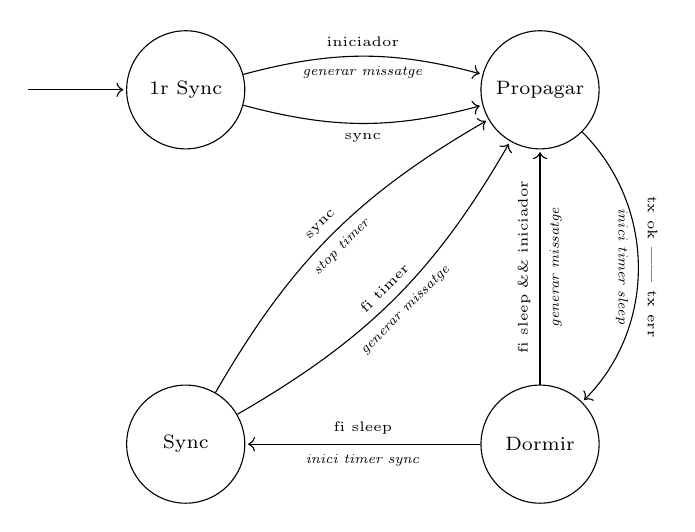
\begin{tikzpicture}[shorten >=1pt, node distance=4.5cm, on grid, auto]
        \tikzstyle{state}=[
            circle,
            draw, 
            minimum size=1.5cm, % uniform size
            inner sep=0pt, 
            align=center
        ]

        \node[state] (first) {\scriptsize 1r Sync};
        \node[state] (prop) [right=of first] {\scriptsize Propagar};
        \node[state] (sleep) [below=of prop] {\scriptsize Dormir};
        \node[state] (sync) [left=of sleep] {\scriptsize Sync};

        \draw[->] (-2,0) -- (first);

        \path[->]
        (first) edge[bend left=15] node {\tiny iniciador} node[below] {\tiny \emph{generar missatge}} (prop)
        (first) edge[bend right=15] node[below] {\tiny sync} (prop)

        (prop) edge[bend left=45] 
            node[sloped, above] {\tiny tx ok || tx err} 
            node[sloped, below] {\tiny \emph{inici timer sleep}} 
        (sleep)

        % (prop) edge[bend right=15] node[sloped, above] {\tiny tx err} (sleep)
        
        (sleep) edge node[above] {\tiny fi sleep} node {\tiny \emph{inici timer sync}}  (sync)
        (sleep) edge 
            node[sloped, above] {\tiny fi sleep \&\& iniciador}
            node[sloped, below] {\tiny \emph{generar missatge}}
            (prop)


        (sync) edge[bend left=15] node[sloped, above] {\tiny sync} node[sloped, below] {\tiny \emph{stop timer}} (prop)
        (sync) edge[bend right=15] node[sloped, above] {\tiny fi timer}
            node[sloped, below] {\tiny\emph{generar missatge}}
            (prop);

    \end{tikzpicture}
    \caption{Diagrama de la màquina d'estats de la capa d'aplicació.}
    \label{fig:app_maquina_estats}
\end{figure}

\subsection{Utilització}
Aquest apartat descriu com utilitzar l'aplicació de baix consum, i la seva implementació en una xarxa de dispositius. Tot i que el funcionament de la sincronització i propagació de dades és automàtic, existeixen determinades operacions que requereixen intervenció manual. Es proporciona també un exemple de funcionament mínim de l'aplicació.

\subsubsection{Configuració inicial}
Un cop es disposa de la xarxa de dispositius establerta i dissenyada, cal configurar de forma individual cada dispositiu per indicar-li quin és el seu dispositiu veí, al qual li ha de propagar els missatges. També cal indicar-li si és el dispositiu de referència, i la quantitat de dispositius de la xarxa.

Amb tots els dispositiu correctament configurats i programats, es pot iniciar el sistema. Els dispositius s'han d'iniciar de forma inversa a com es propaguen les dades, és a dir, començant pel dispositiu més llunyà al de referència (i més proper al \est{gateway}), i acabant pel de referència. Això és necessari per garantir que cada dispositiu trobi el seu veí actiu quan s'inicia, i redueix el temps que els dispositius es troben en l'estat d'espera de sincronització inicial. Si s'iniciés en l'ordre contrari, el dispositiu de referència començaria a transmetre quan la resta encara estrarien apagats. En encendre'ls posteriorment, aquests quedarien esperant una sincronització que ja s'hauria produït, i haurien de romandre actius gairebé tot un cicle complet abans de rebre'l.

Es vol destacar el fet que els dispositius no estan restringits a haver de transmetre tots la mateixa quantitat de dades. Així, un dispositiu podria estar configurat per haver de transmetre \SI{2}{\byte}, mentre que un altre \SI{10}{\byte}. Tot i això, aquesta situació requeriria més complexitat en el servidor d'aplicació LoRaWAN encarregat de descodificar les dades, que hauria de considerar aquestes longituds diferents. 
% // TODO: A PARTIR D'AQUI QUEDA PENDENT REVISAR

\subsubsection{Configuració de nous dispositius}
Pot haver de ser necessari afegir nous dispositius a la xarxa. En aquest cas, es distingeixen dues situacions depenent del rol del dispositiu a afegir:
\begin{itemize}
    \item \emph{Referència}. Si es vol afegir un dispositiu nou a l'extrem més allunyat al \est{gateway}, aquest serà el de referència. 
    \begin{enumerate}
        \item Configurar el nou dispositiu amb el rol de referència, i indicar-li qui és el seu veí a qui ha d'enviar les dades.
        \item Configurar l'antic dispositiu de referència, per indicar-li que ja no té aquest rol. El seu veí no es veu modificat, continua sent el mateix.
        \item Resincronitzar tots els dispositius de la xarxa, aturant-los tots i tornant-los a iniciar en l'ordre vist anteriorment.
    \end{enumerate}

    \item \emph{No referència}. Si es vol afegir un dispositiu nou a la xarxa, però no és el de referència, cal seguir els següents passos:
    \begin{enumerate}
        \item Configurar el nou dispositiu indicant-li qui és el seu veí a qui ha d'enviar les dades.
        \item Reconfigurar el dispositiu anterior al nou, per indicar-li la nova adreça del seu veí, que ara és la del dispositiu nou. 
        \item Iniciar ambdós dispositius, que entraran en mode de recepció de forma indefinida fins a rebre la primera sincronització. 
    \end{enumerate}
\end{itemize}

És important considerar que la capa d'aplicació necessita conèixer la quantitat de dispositius anteriors al que s'afegeix per calcular correctament el temps de tolerància (veure \autoref{eq:app_tolerancia}). 

Si la quantitat de dispositius anteriors és major que la que s'ha configurat, el càlcul del temps de tolerància serà incorrecte, i no es pot garantir la sincronització. Si això passés, seria necessari modificar aquest paràmetre en tots els dispositius següents al que s'afegeix, i reiniciar-los tots. Pel que fa als dispositius anteriors, aquest valor seria el mateix i, per tant, no és necessari modificar-lo. Per aquest motiu, si es té pensat afegir nous dispositius, es recomana establir aquest paràmetre un valor superior al necessari.

Això es pot evitar si els dispositius s'afegeixen únicament en l'extrem del \est{gateway}, ja que aquest seria l'últim dispositiu de la cadena. Llavors, seria únicament necessari modificar el dispositiu anterior al que s'afegeix per indicar-li el nou veí, i establir que no té capacitats LoRaWAN.

\subsubsection{Resincronització de la xarxa}
Tot i que l'aplicació intenta garantir la sincronització de tots els dispositius de la xarxa, i la robustesa i fiabilitat, és possible que es produeixin errors que puguin dur a una desincronització total de la xarxa. En tal cas, caldria reiniciar tots els dispositius de la xarxa, i iniciar-los de nou com si fos la primera vegada. En aquest procediment també es recomana detectar l'error que ha provocat la desincronització, i corregir-lo si és possible. A continuació es mostren algunes possibles causes d'error, i la seva solució:
\begin{itemize}
    \item Mal enllaç entre dispositius. Si la desincronització és causada per un mal enllaç entre dispositius, es podrien modificar els paràmetres de transmissió LoRa, o bé afegir un dispositiu intermig per millorar la comunicació.
    \item Sincronització rebuda en baix consum. Si la sincronització es rep quan el dispositiu encara es troba en mode de baix consum, és possible que el temps de marge, encarregat de contrarestar l'error del rellotge, sigui massa petit. 
    \item Consums excessius. Si es detecta que un dispositiu té consums d'energia excessius i dispars amb la resta, pot ser causat a reinicis del microcontrolador, fent que es quedi en mode de sincronització inicial. És important verificar que l'alimentació del dispositiu és suficient per alimentar el microcontrolador i el mòdul de comunicació, que pot tenir un consum elevat en el moment de la transmissió.
\end{itemize}

\subsubsection{Exemple}
\label{subsubsec:exemple_app}
A continuació es presenta un exemple de funcionament mínim de l'aplicació. Es mostra com configurar la capa d'aplicació, i com implementar el \emph{callback} encarregat d'obtenir les dades a transmetre. Seguidament, es mostra un exemple de descodificador d'\est{uplinks} al servidor d'aplicació, configurable a través del portal de \acro{ttn}. Aquest mostra la informació del paquet (estructura de dades de la capa d'encaminament), que a les seves dades conté el segment de transport i les dades del missatge d'aplicació.

\begin{lstlisting}[style=cppStyle, caption={Exemple de funcionament mínim de l'aplicació de baix consum.}]
#include "sleep.h"
#include "transport.h"

#define SLEEP_IS_INITIATOR false

void getData(uint8_t* data, size_t size) {
    // Omplir `size` bytes amb dades.
    // Aqui es farien lectures
    for(int i = 0; i < size; i++) {
        data[i] = esp_random() % 256;
    }
}

void setup() {
    // Iniciar stack protocol
    if(!Transport_init(NODE_ADDRESS, IS_GATEWAY))
        while(1) delay(1);

    RoutingTable_addRoute(0x02, 0x02); // Configurar taula rutes
    Sleep_onSync(getData); // Configurar callback dades
    Sleep_setForwardNode(0x02); // Configurar node a propagar

    if(!Sleep_init()) // Iniciar aplicacio
        while(1) delay(1);
}

void loop() {
    scheduler_run(); // Unic metode a executar a loop
}
\end{lstlisting}

\begin{lstlisting}[style=jsStyle, caption={Exemple de descodificador de dades al servidor d'aplicació.}]
function decodeUplink(input) {
    var data = {};

    data.src = input.bytes[0];
    data.dest = input.bytes[1];
    data.ttl = input.bytes[2];
    data.dataLen = input.bytes[3]
    data.transport = {};
    data.transport.flags = {};
    data.transport.id = (input.bytes[5]<<8)+(input.bytes[4]);
    //data.transport.flags.raw = input.bytes[6];
    data.transport.flags.ackreq = input.bytes[6] & 0x01;
    data.transport.flags.ackresp = (input.bytes[6] & 0x02) >>> 1;
    data.transport.flags.port = (input.bytes[6] & 0xFC) >>> 2;
    data.transport.dataLen = input.bytes[7];
    data.transport.data = input.bytes.slice(8, 8 + data.transport.dataLen);
    return {
        data: data
    };
}
\end{lstlisting}

\subsection{Validació i resultats}
\subsubsection{Entorn de proves}
Les proves s'han realitzat utilitzant dos microcontroladors ESP32, juntament amb el transductor LoRa \acro{sx1262}. Per verificar el correcte funcionament a través de LoRaWAN, es disposava també de connectivitat a un \est{gateway} Mikrotik wAP-LR8.

S'ha utilitzat el codi d'exemple mostrat al \autoref{subsubsec:exemple_app}, tant per als microcontroladors com per al descodificador de dades al portal de \acro{ttn}. El nivell de les traces utilitzat, definit mitjançant l'opció \fitx{LOG_LEVEL}, és el nivell 1, que correspon al nivell d'informació. Això permet veure la màxima quantitat de 
traces, facilitant-ne l'anàlisi i detecció d'errors.

Per verificar el correcte funcionament de l'aplicació de baix consum, s'ha afegit un punt de depuració específic amb el prefix \fitx{[SLEEP_STATS]}. Aquest punt proporciona informació detallada sobre els temps de sincronització, la finalització del cicle de funcionament, el temps de baix consum i l'estat de sincronització, entre d'altres. Aquesta informació es transmet a través del port sèrie, i es pot observar en temps real mitjançant eines com \est{picocom}.

Per afegir marques temporals (\emph{timestamps}) a cada línia de sortida, s'ha utilitza l'eina \emph{ts}, la qual permet registrar l'instant en què s'ha rebut cada missatge. Amb aquesta informació és possible determinar si els cicles de baix consum es realitzen correctament. A més, aquesta informació s'ha redirigit a un fitxer per al seu posterior anàlisi. L'ordre utilitzada per obtenir aquesta informació és la següent:

\begin{lstlisting}[style=bashStyle]
picocom --omap spchex,tabhex,crhex,lfhex --baud 115200 --imap lfcrlf <port_UBS> | ts "[%Y-%m-%d %H:%M:%.S]" >> <nom_fitxer>
\end{lstlisting}

\subsubsection{Proves}
Abans d'iniciar les proves, es va comprovar quin era l'error del rellotge dels microcontroladors en mode de baix consum. Es va fer un petit programa que posava el dispositiu en mode de baix consum durant un temps conegut, enviant un missatge de depuració abans i després d'aquest mode. Gràcies a les marques de temps, era possible determinar la durada real del mode de baix consum, i determinar l'error en \acro{ppm} a partir de la durada esperada. Aquest experiment es va repetir per a diferents temps de cicle, i múltiples vegades. Es pot observar el codi i els resultats obtinguts a la carpeta \fitx{tests/CalculErrorPPM}.

Per a cada microcontrolador, l'error obtingut va ser de -4700 \acro{ppm} i -5700 \acro{ppm}. Així, el temps transcorregut «real» és menor al que el rellotge intern considera: si li indiquem que estigui en mode de baix consum durant 1 minut, realment hi estarà $1+1\cdot (-5700)\cdot10^-6=0.994$ minuts, considerant l'error del segon dispositiu. 
\newline
\newline
Es va començar realitzant proves amb un temps de cicle de 5 minuts. A partir de l'error dels rellotges, es va determinar el temps de marge ($t_m$) a través de l'expressió \ref{eq:temps_marge}, obtenint que $t_m \ge 1.71$, i establint-lo a 2 segons. 

La situació dels dispositius era la següent:
\begin{itemize}
    \item \emph{Dispositiu 1}. El dispositiu de referència, amb adreça \fitx{0x03}. Té definit el dispositiu \fitx{0x02} com a veí.
    \item \emph{Dispositiu 2}. Té capacitats LoRaWAN. Espera rebre el missatge de dades, i té definida l'adreça \fitx{0x01} ---l'adreça virtual del \est{gateway}--- com a veí.
\end{itemize}

% aqui parlar de l'error del clock?
\chapter{Conclusions}
% \section{Resultats assolits}
% \section{Limitacions del disseny final}
% \section{Punts clau de millora}

\chapter{Treball futur}
% \section{Suport a topologies més complexes}
% \section{Optimització del consum energètic}
% \section{Integració amb LoRaWAN o altres protocols}

% fragmentació a nivell de protocol o a nivell d'aplicació
% configuració dinàmica de dispositius
% 

% \listoftables

\printbibliography


% Si feu servir apèndixs, descomenteu
% (també la  \part del principi del document)
%\appendix
%\part{Apèndixs}
%\chapter{Un apèndix}


% ABANS D'ENTREGAR MIRAR QUE L·L ESTIGUIN BEN ESCRITES AMB \l.l
% // TODO: Falta diagrama FSM de capa MAC
% // TODO: Diagrama funcionament transport

% // TODO: Modiciar ’ per '

% « »
% « »
% « »
% « »
% « »
% « »
% « »
% « »

\end{document}

%%% Local Variables:
%%% mode: latex
%%% TeX-master: t
%%% LaTeX-biblatex-use-Biber: t
%%% End: